\def\micro{\mu m}
\def\um{$\micro$ }
\def\degreesC{$\degree C$ }
\def\percent{$\%$ }
\documentclass[10pt,a4paper,oneside]{article}
\usepackage[left=2cm,right=2cm,top=2cm,bottom=2cm]{geometry}

\usepackage[dvipsnames]{xcolor}

%%  -------------------------------------------------------------------
%%      GDS II layer, regarding MOSIS SCMOS layer map
%%  -------------------------------------------------------------------
% GDS II #41 - P_WELL
\definecolor{pwell}{rgb}{1.0, 0.74, 0.53}   % macaroni and cheese
% GDS II #42 - N_WELL
\definecolor{nwell}{rgb}{0.61, 0.87, 1.0}  % columbia blue
\definecolor{pbase}{rgb}{1.0, 0.51, 0.26}  % mango tango
\definecolor{nbase}{rgb}{0.0, 0.75, 1.0}   % capri 
% GDS II #43 - ACITVE
\definecolor{active}{rgb}{0.9, 0.4, 0.38}   % light carmine pink
% GDS II #45 - N_PLUS_SELECT
\definecolor{nimplant}{rgb}{0.45, 0.76, 0.983}% maya blue
% GDS II #44 - P_PLUS_SELECT
\definecolor{pimplant}{rgb}{1.0, 0.51, 0.26}% mango tango
% GDS II #46 - POLY
\definecolor{poly}{rgb}{0.56, 0.93, 0.56}   % light green
% GDS II #25 - CONTACT
\definecolor{contact}{rgb}{0.83, 0.83, 0.83}% light gray
% GDS II #49 - METAL1
\definecolor{metal1}{rgb}{0.38, 0.31, 0.86} % majorelle blue
% GDS II #50 - VIA1
\definecolor{via1}{rgb}{0.83, 0.83, 0.83}   % light gray
% GDS II #51 - METAL2
\definecolor{metal2}{rgb}{0.04, 0.85, 0.32} % malachite
% GDS II #61 - VIA2
\definecolor{via2}{rgb}{0.83, 0.83, 0.83}   % light gray
% GDS II #63 - METAL3
\definecolor{metal3}{rgb}{0.98, 0.93, 0.37} % maize
% GDS II #30 - VIA3
\definecolor{via3}{rgb}{0.83, 0.83, 0.83}   % light gray
% GDS II #31 - METAL4
\definecolor{metal4}{rgb}{0.75, 0.25, 0.0}  % mahogany
% GDS II #32 - VIA4
\definecolor{via4}{rgb}{0.83, 0.83, 0.83}   % light gray
% GDS II #33 - METAL5
\definecolor{metal5}{rgb}{0.79, 0.08, 0.48} % magenta (dye)
% GDS II #36 - VIA5
\definecolor{via5}{rgb}{0.83, 0.83, 0.83}   % light gray
% GDS II #37 - METAL6
\definecolor{metal6}{rgb}{0.11, 0.35, 0.02} % lincoln green
% GDS II #29 - SILICIDE_BLOCK
\definecolor{silicide-block}{rgb}{0.98, 0.94, 0.9}  % linen
% GDS II #52 - GLASS
\definecolor{glass}{rgb}{1.0, 1.0, 0.88}    % light yellow
% GDS II #26 - PADS
\definecolor{pads}{rgb}{0.75, 1.0, 0.0}     % lime (color wheel)

\definecolor{resist}{rgb}{0.71, 0.4, 0.11}  % light brown

\definecolor{silicide}{rgb}{0.29, 0.33, 0.13}
\definecolor{titanium}{rgb}{0.8, 0.58, 0.46}

\def\OpacityLayout {0.5}

%
% physical
%
\definecolor{substrate}{rgb}{0.96, 0.94, 0.93}  % isabelline
\definecolor{nitride}{rgb}{1.0, 0.03, 0.0}
\definecolor{gateoxide}{rgb}{0.88, 1.0, 1.0}    % light cyan
\definecolor{isolationoxide}{rgb}{0.84, 0.79, 0.87}% languid lavender

\usepackage[utf8]{inputenc}
\usepackage[english]{babel}
\usepackage{forloop}
\usepackage{amsmath}
\usepackage{amsfonts}
\usepackage{amssymb}
\usepackage{gensymb}
\usepackage{mdframed}
\usepackage{graphicx}
\usepackage{tikz}
\usetikzlibrary{arrows,automata,shapes}
\usepackage[siunitx]{circuitikz}
\usepackage{makecell}
\usepackage{array}

\def\WaferClean{
\begin{tikzpicture}\node [fill=cyan, rounded corners=5pt] {Clean};\end{tikzpicture}}
\def\WaferSemiClean{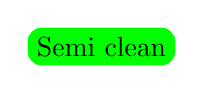
\begin{tikzpicture}\node [fill=green, rounded corners=5pt] {Semi clean};\end{tikzpicture}}
\def\WaferNonStandard{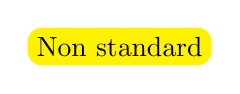
\begin{tikzpicture}\node [fill=yellow, rounded corners=5pt] {Non standard};\end{tikzpicture}}

\usepackage[colorlinks=true,linkcolor=blue,urlcolor=black,bookmarksopen=true]{hyperref}
\usepackage{bookmark}
\usepackage{hyperref}
\usepackage{sepfootnotes}
\usepackage{lipsum,tocloft} 
\usetikzlibrary{positioning}
\usetikzlibrary{patterns}

\usepackage{float}
\floatstyle{boxed} 
\restylefloat{figure}

\title{Libre Silicon process steps}
\date{\today}
\author{David Lanzendörfer}
\makeindex

\newcounter{ct}
\def\CrossSectionOnly{0.3}
\def\CrossAndTopSection{0.2}
\def\CrossAndTopSectionBig{0.3}
\def\VLSILayout{0.4}

\DeclareMathOperator\erfc{erfc}

\setlength{\parindent}{0pt} % get rid of annoying indents

\begin{document}
\begin{abstract}
	Copyright © 2017 LANCEVILLE TECHNOLOGY GROUP CO., LIMITED. All rights reserved. \\

This process is licensed under the Libre Silicon public license; you can redistribute it and/or modify it under the terms of the Libre Silicon public license
as published by the Libre Silicon alliance, either version 1 of the License, or (at your option) any later version.

This design is distributed in the hope that it will be useful, but WITHOUT ANY WARRANTY; without even the implied warranty of MERCHANTABILITY or FITNESS FOR A PARTICULAR PURPOSE.
See the Libre Silicon Public License for more details. \\

This document is part of the specification of the free silicon manufacturing standard for manufacturing the LibreSilicon standard logic cells\footnote{\url{https://github.com/chipforge/StdCellLib}} and related free technology nodes from the LibreSilicon project.

For this initial revision 0.1 a gate-first approach has been chosen which led to the choice of polysilicon as the gate electrode material because of the simplicity of the gate alignment.
For better isolation properties of the transistors and gates in overall a box-isolation approach has been chosen.
All of these choices have been made with the future scale down from the recent $1 \mu m$ to smaller structure sizes.
\textbf{This process is for manufacturing $1 \mu m$ only!}
But further releases which will have been tested with smaller structure sizes can be expected.

\end{abstract}
\newpage
\maketitle
\tikzstyle{block} = [rectangle, draw, fill=blue!20, text width=3cm, text centered, rounded corners, minimum height=1.5cm]
\tikzstyle{line} = [draw, very thick, color=black!50, -latex']

The general flow chart of the overall process flow can be seen in \autoref{full_flow}.
These process steps will be discussed within the following sections.
\begin{figure}[H]
	\centering
	\begin{tikzpicture}[node distance=2cm, thick,scale=0.8, every node/.style={transform shape}]
		%% Place nodes
		%active CMOS				
		\node [block] (isolation) at (4,20) {Isolation (STI)\\ \autoref{sti}};
		\node [block, below of=isolation] (nwell) {N-Well\\ \autoref{nwell_chapter}};
		\node [block, below of=nwell] (pwell) {P-Well\\ \autoref{pwell_chapter}};
		\node [block, below of=pwell] (gate) {Gate\\ \autoref{gate}};
		\node [block, below of=gate] (np) {n+ Implant\\ \autoref{nimplant}};
		\node [block, below of=np] (pp) {p+ Implant\\ \autoref{pimplant}};
		\node [block, below of=pp] (silicification) {Silicification\\ \autoref{step_silicification}};
		%post proces
		\node [block] (via1) at (8,8) {First vias\\ \autoref{via1}};
		\node [block, above of=via1] (metal1) {First metal\\ \autoref{metal1}};
		\node [block, above of=metal1] (via2) {Additional vias\\ \autoref{via2}};
		\node [block, above of=via2] (metal2) {Additional metal\\ \autoref{metal2}};
		\node (repeat) at (10.5,14.5) {Repeat};

		%% Draw edges
		\path [line] (isolation) -- (nwell);
		\path [line] (nwell) -- (pwell);
		\path [line] (pwell) -- (gate);
		\path [line] (gate) -- (np);
		\path [line] (np) -- (pp);
		\path [line] (pp) -- (silicification);
		\path [line] (silicification) -- (via1);
		\path [line] (via1) -- (metal1);
		\path [line] (metal1) -- (via2);
		\path [line] (via2) -- (metal2);
		\path [line] (metal2) -- +(3,0) -- +(3,-2) -- (via2);

		\draw[dotted] (2,6) rectangle (6,21);
		\node at (4,6.5) {CMOS process};
		\draw[dotted] (6,6) rectangle (12,21);
		\node at (8,6.5) {Interconnect};

		%\draw[dotted] (1.5,9) rectangle (10.5,21.5);
		%\node at (4,9.5) {Front-end processing};

		%\draw[dotted] (11,9) rectangle (15,21.5);
		%\node at (13,9.5) {Back-end processing};
	\end{tikzpicture}
	\caption{Frontend and backend process flow}
	\label{full_flow}
\end{figure}
The six overall process steps are part of an active part of the technology, while the final metal (respectively contact) layers will be used for making a contact between the logic gates and macro cells and making them available to the exterior world.

For this process p-substrate is the required basic substrate, but forks and modifications will be very well possible based on a Graphene substrate or alike, still under the LSPL.
The starting material is a p-type, <100> oriented silicon with a doping concentration of $\approx 9\times10^{14}cm^{-3}$.\\



\label{process_overview}
\newpage
\section{Shallow trench isolation}\label{sti_chapter}
The geometry of a substrate with STI implemented can be seen in \autoref{sti_target}.

\begin{figure}[H]
	\centering
	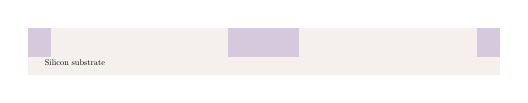
\begin{tikzpicture}[node distance = 3cm, auto, thick,scale=\CrossAndTopSectionBig, every node/.style={transform shape}]
		% substrate
\fill[substrate] (0,0) rectangle (20,2);
\node at (2,0.5) {Silicon substrate};
%trenches
\fill[isolationoxide] (0,0.75) rectangle (1,2);
\fill[isolationoxide] (8.5,0.75) rectangle (11.5,2);
\fill[isolationoxide] (19,0.75) rectangle (20,2);
	\end{tikzpicture}
	
\begin{tikzpicture}[node distance = 3cm, auto, thick,scale=\CrossAndTopSectionBig, every node/.style={transform shape}]
		% substrate
\fill[YellowOrange] (0,0) rectangle (20,12);
% trench area
\fill[DarkGray] (0,0) rectangle (1,12);
\fill[DarkGray] (8.5,0) rectangle (11.5,12);
\fill[DarkGray] (19,0) rectangle (20,12);
\fill[DarkGray] (0,0) rectangle (20,1.25);
\fill[DarkGray] (0,7.5) rectangle (20,12);
	\end{tikzpicture}
	\caption{Shallow trench isolation target geometry}
	\label{sti_target}
\end{figure}

As can be seen in \autoref{nwell_target}, the n-well and the STI trench are supposed to have approximately the same depth but the n-well and p-well go down a little bit further.
Because the n-well will be $\approx 4 \mu m$ in depth we have to match this with our trench depth.
I order to allow a sufficiently low resistance of the ESD diode but at the same time a sufficient isolation of between the standard cells a trade-ff has been done.
The targeted depth of the box isolation is $\approx 2 \mu m$.

\begin{figure}[H]
	\centering
	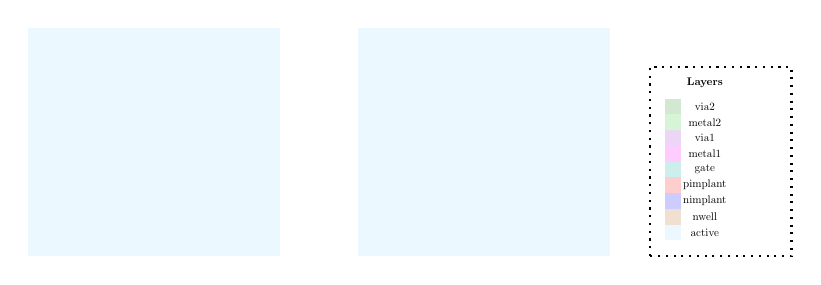
\begin{tikzpicture}[node distance =1cm, auto, thick,scale=\VLSILayout, every node/.style={transform shape}]
		\fill[nwell,opacity=0.2] (0.75,0.5) rectangle (8.75,7.75);
\fill[nwell,opacity=0.2] (11.25,0.5) rectangle (19.25,7.75);

\draw[dotted] (20.5,0.5) rectangle (25,6.5);

\node at (22.25,6) {\textbf{Layers}};

\fill[nwell,opacity=0.2] (21,1) rectangle (21.5,1.5);
\node at (22.25,1.25) {active};

\fill[resist,opacity=0.2] (21,1.5) rectangle (21.5,2);
\node at (22.25,1.75) {nwell};

\fill[blue,opacity=0.2] (21,2) rectangle (21.5,2.5);
\node at (22.25,2.25) {nimplant};

\fill[nitride,opacity=0.2] (21,2.5) rectangle (21.5,3);
\node at (22.25,2.75) {pimplant};

\fill[Emerald,opacity=0.2] (21,3) rectangle (21.5,3.5);
\node at (22.25,3.25) {gate};

\fill[Fuchsia,opacity=0.2] (21,3.5) rectangle (21.5,4);
\node at (22.25,3.75) {metal1};

\fill[DarkOrchid,opacity=0.2] (21,4) rectangle (21.5,4.5);
\node at (22.25,4.25) {via1};

\fill[LimeGreen,opacity=0.2] (21,4.5) rectangle (21.5,5);
\node at (22.25,4.75) {metal2};

\fill[ForestGreen,opacity=0.2] (21,5) rectangle (21.5,5.5);
\node at (22.25,5.25) {via2};

	\end{tikzpicture}
	\caption{Shallow trench isolation layout}
	\label{sti_layout}
\end{figure}

In \autoref{sti_layout} we can see the layout for the STI area.
The STI area will be everywhere, where no active areas are.
The field oxide needs to be grown out of trenches which can't been etched out of the silicon by using resist as a mask.
For that reason we will have to resort to a protective mask made from a silicon dioxide layer which has to be etched before hand.
So the mask will be exposed onto positive resist on top of the hard mask oxide layer in order to form a protective mask covering the active areas from having etched trenches into them..
After that we can either use a dry etching method or wet etching for cutting into the silicon substrate and making the active area become islands with trenches in between.
After these steps we have to remove the hard mask.
Our minimum width and height as well as the space between the active areas comes from the line space constrain of the silicon etcher and of course the optical limitations of the stepper which are as well 0.5\um.

\newpage

\subsection{Initial cleaning}
In order to remove the initial naturally grown silicon dioxide from the wafer, acid is being applied to the wafer which leads to a pure silicon substrate wafer as in the process illustration shown in \autoref{initial_cleaning}.

\begin{figure}[H]
	\centering
	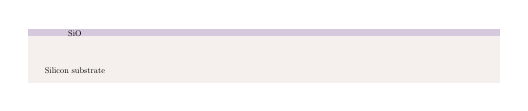
\begin{tikzpicture}[node distance = 3cm, auto, thick,scale=\CrossSectionOnly, every node/.style={transform shape}]
		% substrate
\fill[substrate] (0,0) rectangle (20,2);
\node at (2,0.5) {Silicon substrate};
% oxide
\fill[isolationoxide] (0,2) rectangle (20,2.3);
\node at (2,2.1) {SiO};
	\end{tikzpicture} \\
	
\includegraphics[scale=0.01]{down_arrow.png} \\
	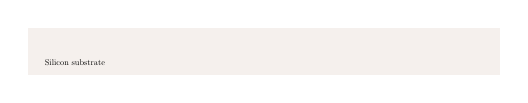
\begin{tikzpicture}[node distance = 3cm, auto, thick,scale=\CrossSectionOnly, every node/.style={transform shape}]
		% substrate
\fill[substrate] (0,0) rectangle (20,2);
\node at (2,0.5) {Silicon substrate};
	\end{tikzpicture}
	\caption{Initial cleaning}
	\label{initial_cleaning}
\end{figure}

This needs to be done because the naturally grown initially existing silicon oxide is not pure and may contain contamination which may render the final product unusable.

\subsubsection{Sulfuric Cleaning}
The sulfuric acid mixture, $H_2 S O_4 + H_2 O_2$ is being applied to the wafer for 10 minutes at a temperature of 120 \degree C.

\subsubsection{HF dip}
After the sulfuric cleaning a HF (HF:$H_2O$,1:50) dip is being performed for one minute. \\
Hydrofluoric acid (HF) is used to remove native silicon dioxide from wafers. Since it acts quickly, one needs to only expose the wafer for a short time ("dip").

\subsubsection{Drying}
After that the wafer needs to be dried and quickly processed further before new uncontrolled natural oxide can build up on the wafer through the contact with air.

\subsection{Hard mask: Oxide growth}
We need a thick layer of oxide as protective hard mask to etch the trenches into the silicon.

\begin{figure}[H]
	\centering
	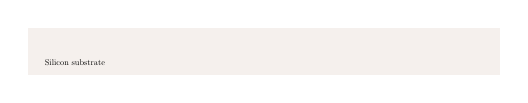
\begin{tikzpicture}[node distance = 3cm, auto, thick,scale=\CrossSectionOnly, every node/.style={transform shape}]
		% substrate
\fill[substrate] (0,0) rectangle (20,2);
\node at (2,0.5) {Silicon substrate};
	\end{tikzpicture} \\
	
\includegraphics[scale=0.01]{down_arrow.png} \\
	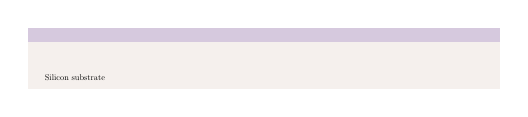
\begin{tikzpicture}[node distance = 3cm, auto, thick,scale=\CrossSectionOnly, every node/.style={transform shape}]
		% substrate
\fill[substrate] (0,0) rectangle (20,2);
\node at (2,0.5) {Silicon substrate};
\fill[isolationoxide] (0,2) rectangle (20,2.6);
	\end{tikzpicture}
	\caption{Hard mask growth}
\end{figure}

Because we want to etch 2\um deep into the silicon which takes 4 minutes and 30 seconds using KOH acid at 60\degreesC in \autoref{sti_trench_etch}.

This means the oxide layer needs to be at least 226 nm thick, so we choose a nice round number of 300nm.

The layer of silicon dioxide of around 300nm thickness is grown in wet ambient for 25 minutes at 1050\degreesC\footnote{\url{http://cleanroom.byu.edu/OxideTimeCalc}} in the diffusion furnace.

\newpage

\subsection{Hard mask: Patterning}

The resist is being deposited using spin coating and then baked depending on the baking time for the specific resist.

\begin{figure}[H]
	\centering
	\begin{tikzpicture}[node distance = 3cm, auto, thick,scale=\CrossSectionOnly, every node/.style={transform shape}]
		\input{tikz_process_steps/sti.hard_mask_oxide_growth.a.tex}
\fill[isolationoxide] (0,2) rectangle (20,2.6);
	\end{tikzpicture} \\
	
\includegraphics[scale=0.01]{down_arrow.png} \\
	\begin{tikzpicture}[node distance = 3cm, auto, thick,scale=\CrossSectionOnly, every node/.style={transform shape}]
		\input{tikz_process_steps/sti.hard_mask_oxide_growth.a.tex}
\fill[isolationoxide] (0,2) rectangle (20,2.6);
\fill[resist] (1,2.6) rectangle (8,3.2);
\fill[resist] (11.5,2.6) rectangle (19,3.2);
	\end{tikzpicture}
	\caption{Patterning with positive resist}
\end{figure}

The layout for being exposed onto the resist is being extracted from the "active" layer within the GDS2 file onto a dark field mask.

A dark field mask can be used because alignment doesn't play a role yet because it's the first layer, however the alignment crosses need to be included into the mask.

\subsection{Hard mask: Etching}\label{sti_mask_etch}

We open the access to the silicon outside of the active areas in order to etch the trenches.

\begin{figure}[H]
	\centering
	\begin{tikzpicture}[node distance = 3cm, auto, thick,scale=\CrossSectionOnly, every node/.style={transform shape}]
		\input{tikz_process_steps/sti.hard_mask_oxide_growth.b.tex}
\fill[resist] (1,2.6) rectangle (8,3.2);
\fill[resist] (11.5,2.6) rectangle (19,3.2);
	\end{tikzpicture} \\
	
\includegraphics[scale=0.01]{down_arrow.png} \\
	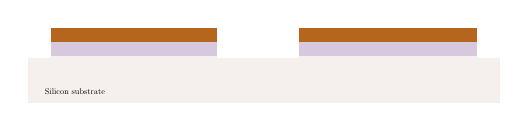
\begin{tikzpicture}[node distance = 3cm, auto, thick,scale=\CrossSectionOnly, every node/.style={transform shape}]
		% substrate
\fill[substrate] (0,0) rectangle (20,1.9);
\node at (2,0.5) {Silicon substrate};

% substrate islands
\fill[substrate] (1,1.9) rectangle (8,2);
\fill[substrate] (11.5,1.9) rectangle (19,2);

% pad oxide
\fill[isolationoxide] (1,2) rectangle (8,2.6);
\fill[isolationoxide] (11.5,2) rectangle (19,2.6);

% resist
\fill[resist] (1,2.6) rectangle (8,3.2);
\fill[resist] (11.5,2.6) rectangle (19,3.2);
	\end{tikzpicture}
	\caption{Nitride mask etching}
\end{figure}

There are dry etching and wet etching methods available for etching the oxide hard mask. The downside of wet etching is that it also etches horizontally, however the chemical BHF is readily available and allows for easy implementation of the process.\\

\textbf{Possible approaches}:
\begin{itemize}
	\item \textbf{"DRIE Etcher \#1" from HKUST} \\
	We can use anisotropic plasma etching for sharper borders.
	\item \textbf{Chemical solution} \\
	We can use buffered hydrofluoric acid (BOE (1:6)) at room temperature for a little bit over 3 minutes in order to get through the 300nm of oxide.\\
	Too long over 3 minutes might cause under-etch however!
\end{itemize}

\subsection{Hard mask: Resist removal}
Now we need to remove the contaminants for further processing.

\begin{figure}[H]
	\centering
	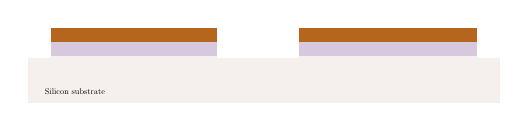
\begin{tikzpicture}[node distance = 3cm, auto, thick,scale=\CrossSectionOnly, every node/.style={transform shape}]
		% substrate
\fill[substrate] (0,0) rectangle (20,1.9);
\node at (2,0.5) {Silicon substrate};

% substrate islands
\fill[substrate] (1,1.9) rectangle (8,2);
\fill[substrate] (11.5,1.9) rectangle (19,2);

% pad oxide
\fill[isolationoxide] (1,2) rectangle (8,2.6);
\fill[isolationoxide] (11.5,2) rectangle (19,2.6);

% resist
\fill[resist] (1,2.6) rectangle (8,3.2);
\fill[resist] (11.5,2.6) rectangle (19,3.2);
	\end{tikzpicture} \\
	
\includegraphics[scale=0.01]{down_arrow.png} \\
	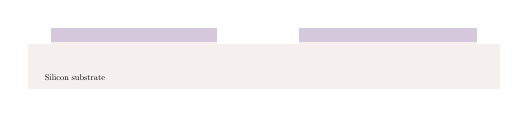
\begin{tikzpicture}[node distance = 3cm, auto, thick,scale=\CrossSectionOnly, every node/.style={transform shape}]
		% substrate
\fill[substrate] (0,0) rectangle (20,1.9);
\node at (2,0.5) {Silicon substrate};

% substrate islands
\fill[substrate] (1,1.9) rectangle (8,2);
\fill[substrate] (11.5,1.9) rectangle (19,2);

% pad oxide
\fill[isolationoxide] (1,2) rectangle (8,2.6);
\fill[isolationoxide] (11.5,2) rectangle (19,2.6);
	\end{tikzpicture}
	\caption{Resist removal}
\end{figure}

We strip the resist, rinse and perform sulfuric cleaning.

\newpage

\subsection{Silicon etching}\label{sti_trench_etch}

Silicon can only be etched by a very aggressive chemical cocktail of  KOH and TMAH (20\%) or by plasma etching.

\begin{figure}[H]
	\centering
	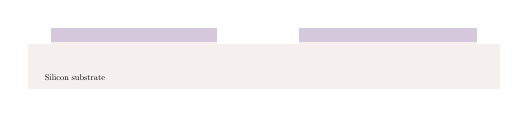
\begin{tikzpicture}[node distance = 3cm, auto, thick,scale=\CrossSectionOnly, every node/.style={transform shape}]
		% substrate
\fill[substrate] (0,0) rectangle (20,1.9);
\node at (2,0.5) {Silicon substrate};

% substrate islands
\fill[substrate] (1,1.9) rectangle (8,2);
\fill[substrate] (11.5,1.9) rectangle (19,2);

% pad oxide
\fill[isolationoxide] (1,2) rectangle (8,2.6);
\fill[isolationoxide] (11.5,2) rectangle (19,2.6);
	\end{tikzpicture} \\
	
\includegraphics[scale=0.01]{down_arrow.png} \\
	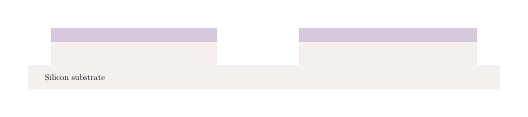
\begin{tikzpicture}[node distance = 3cm, auto, thick,scale=\CrossSectionOnly, every node/.style={transform shape}]
		% substrate
\fill[substrate] (0,0) rectangle (20,1);
\node at (2,0.5) {Silicon substrate};

% substrate islands
\fill[substrate] (1,1) rectangle (8,2);
\fill[substrate] (11.5,1) rectangle (19,2);

% pad oxide
\fill[isolationoxide] (1,2) rectangle (8,2.6);
\fill[isolationoxide] (11.5,2) rectangle (19,2.6);
	\end{tikzpicture}
	\caption{Trench etching}
\end{figure}

\textbf{Possible approaches}:
\begin{itemize}
\item \textbf{"DRIE Etcher \#1" from HKUST} \\
Has a normal etching rate of up to $2\frac{\mu m}{min}$.
This means we etch for 10 minutes with a reduced etch speed of $200\frac{nm}{min}$ in order to be clearly deep enough and to compensate for different etch depths in different places.
This way we have a good chance of having proper isolation everywhere on the wafer.

\item \textbf{Chemical solution} \\
Using a KOH solution of 20\% at 60\degreesC gives us an etch rate of roughly  26.57\um per hour\footnote{\url{http://www.lelandstanfordjunior.com/KOH.html}}.
\begin{itemize}
\item The <100> etch rate is: 26.57 micron/hr = 0.44 micron/min
\item The <110> etch rate is: 40.5 micron/hr 
\item The <111> etch rate is: 0.4932 micron/hr 
\item The SiO2 etch rate is: 49.92 nanometers/hr 
\end{itemize}
With a desired depth of 2\um we will have to etch around 4 minutes and 30 seconds in order to reach the desired depth.
The disadvantage of this approach is the imprecision and under-etch of the mask.
\end{itemize}

\subsection{Hard mask: Removal}

Now we have to remove the oxide hard mask for further processing in order to proceed with well formation without contamination during oxide growing.

\begin{figure}[H]
	\centering
	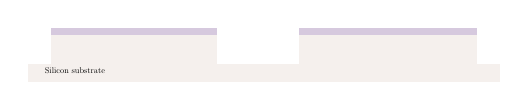
\begin{tikzpicture}[node distance = 3cm, auto, thick,scale=\CrossSectionOnly, every node/.style={transform shape}]
		% substrate
\fill[substrate] (0,0) rectangle (20,0.75);
\node at (2,0.5) {Silicon substrate};

% substrate islands
\fill[substrate] (1,0.75) rectangle (8,2);
\fill[substrate] (11.5,0.75) rectangle (19,2);

% covering oxide
\fill[isolationoxide] (1,2) rectangle (8,2.3);
\fill[isolationoxide] (11.5,2) rectangle (19,2.3);
	\end{tikzpicture} \\
	
\includegraphics[scale=0.01]{down_arrow.png} \\
	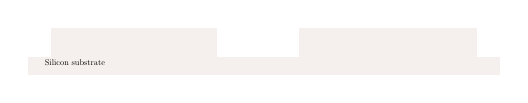
\begin{tikzpicture}[node distance = 3cm, auto, thick,scale=\CrossSectionOnly, every node/.style={transform shape}]
		% substrate
\fill[substrate] (0,0) rectangle (20,0.75);
\node at (2,0.5) {Silicon substrate};

% substrate islands
\fill[substrate] (1,0.75) rectangle (8,2);
\fill[substrate] (11.5,0.75) rectangle (19,2);
	\end{tikzpicture}
	\caption{Trench etching}
\end{figure}

We use buffered hydrofluoric acid (BOE (1:6)) at room temperature for a little bit over 3 minutes in order to remove all of the 300nm thick oxide layer.
\newpage
\section{N-well}\label{nwell_chapter}
In order to build CMOS on the same substrate, an N-well is required for building the complementary P-channel transistor for a n-p-channel logic circuitry as shown above in the example section.
The cross section as well as the top view of the targeted geometry are shown in \autoref{nwell_target}
\begin{figure}[H]
	\centering
	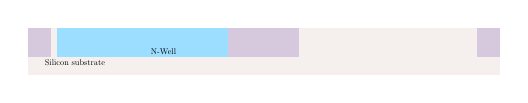
\begin{tikzpicture}[node distance = 3cm, auto, thick,scale=\CrossAndTopSectionBig, every node/.style={transform shape}]
		% substrate
\fill[substrate] (0,0) rectangle (20,2);
\node at (2,0.5) {Silicon substrate};
%trenches
\fill[isolationoxide] (0,0.75) rectangle (1,2);
\fill[isolationoxide] (8.5,0.75) rectangle (11.5,2);
\fill[isolationoxide] (19,0.75) rectangle (20,2);
% n-well
\fill[nwell] (1.25,0.75) rectangle (8.5,2);
\node at (5.75,1) {N-Well};


	\end{tikzpicture}
	
\begin{tikzpicture}[node distance = 3cm, auto, thick,scale=\CrossAndTopSectionBig, every node/.style={transform shape}]
		% substrate
\fill[YellowOrange] (0,0) rectangle (20,12);
% trench area
\fill[DarkGray] (0,0) rectangle (1,12);
\fill[DarkGray] (8.5,0) rectangle (11.5,12);
\fill[DarkGray] (19,0) rectangle (20,12);
\fill[DarkGray] (0,0) rectangle (20,1.25);
\fill[DarkGray] (0,7.5) rectangle (20,12);
\fill[nwell] (1.25,1) rectangle (8.25,7.25);
	\end{tikzpicture}
	\caption{N-well target geometry}
	\label{nwell_target}
\end{figure}

The N-well will serve us as an island of N-doped substrate within the P-doped basis substrate.

The dopant dose will be $2.5\times10^{12}cm^{-2}$ as calculated in the documentation of the process design leading to these steps\footnote{\url{https://github.com/leviathanch/libresiliconprocess/raw/master/process_design/process_design.pdf}}.

\begin{figure}[H]
	\centering
	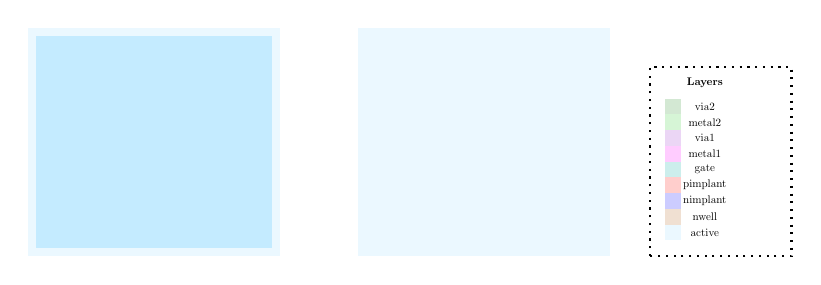
\begin{tikzpicture}[node distance =1cm, auto, thick,scale=\VLSILayout, every node/.style={transform shape}]
		\fill[nwell,opacity=0.2] (0.75,0.5) rectangle (8.75,7.75);
\fill[nwell,opacity=0.2] (11.25,0.5) rectangle (19.25,7.75);

\draw[dotted] (20.5,0.5) rectangle (25,6.5);

\node at (22.25,6) {\textbf{Layers}};

\fill[nwell,opacity=0.2] (21,1) rectangle (21.5,1.5);
\node at (22.25,1.25) {active};

\fill[resist,opacity=0.2] (21,1.5) rectangle (21.5,2);
\node at (22.25,1.75) {nwell};

\fill[blue,opacity=0.2] (21,2) rectangle (21.5,2.5);
\node at (22.25,2.25) {nimplant};

\fill[nitride,opacity=0.2] (21,2.5) rectangle (21.5,3);
\node at (22.25,2.75) {pimplant};

\fill[Emerald,opacity=0.2] (21,3) rectangle (21.5,3.5);
\node at (22.25,3.25) {gate};

\fill[Fuchsia,opacity=0.2] (21,3.5) rectangle (21.5,4);
\node at (22.25,3.75) {metal1};

\fill[DarkOrchid,opacity=0.2] (21,4) rectangle (21.5,4.5);
\node at (22.25,4.25) {via1};

\fill[LimeGreen,opacity=0.2] (21,4.5) rectangle (21.5,5);
\node at (22.25,4.75) {metal2};

\fill[ForestGreen,opacity=0.2] (21,5) rectangle (21.5,5.5);
\node at (22.25,5.25) {via2};

\fill[nwell,opacity=\OpacityLayout] (1,0.75) rectangle (8.5,7.5);
	\end{tikzpicture}
	\caption{N-Well layout}
	\label{nwell_layout}
\end{figure}

In \autoref{nwell_layout} the layout of the n-well region on top of the active area region can be seen.

The n-well is being fit into the active area. It should even be a little bit bigger than the active area, because of possible alignment offsets

\newpage

\subsection{Mask dioxide layer}
In order to selectively inject charge carrying atoms into the crystalline structure a protective dioxide ($SiO_2$) layer needs to be grown on top of a p-type substrate.
\begin{figure}[H]
	\centering
	\begin{tikzpicture}[node distance = 3cm, auto, thick,scale=\CrossSectionOnly, every node/.style={transform shape}]
		\input{tikz_process_steps/pwell.mask_dioxide_layer.a.tex}

% pwell
\fill[pwell] (11.75,0.75) rectangle (18.75,2);
\node at (14.25,1) {P-Well};
	\end{tikzpicture}
	\drawStepArrow{}
	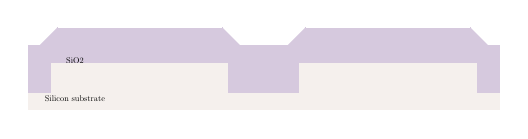
\begin{tikzpicture}[node distance = 3cm, auto, thick,scale=\CrossSectionOnly, every node/.style={transform shape}]
		% oxide
\fill[isolationoxide] (0,1.25) rectangle (20,2.75);

% oxide hill 1
\fill[isolationoxide] (1.25,2.75) rectangle (8.25,3.5);
\filldraw[line width=0, isolationoxide] (0.5,2.75) -- (1.25,2.75) -- (1.25,3.5);
\filldraw[line width=0, isolationoxide] (8.25,2.75) -- (8.25,3.5) -- (9.0,2.75);

% oxide hill 2
\fill[isolationoxide] (11.75,2.75) rectangle (18.75,3.5);
\filldraw[line width=0, isolationoxide] (11.0,2.75) -- (11.75,2.75) -- (11.75,3.5);
\filldraw[line width=0, isolationoxide] (18.75,2.75) -- (18.75,3.5) -- (19.5,2.75);

\node at (2,2.1) {SiO2};

% substrate
\fill[substrate] (0,0) rectangle (20,2);
\node at (2,0.5) {Silicon substrate};
%trenches
\fill[isolationoxide] (0,0.75) rectangle (1,2);
\fill[isolationoxide] (8.5,0.75) rectangle (11.5,2);
\fill[isolationoxide] (19,0.75) rectangle (20,2);
	\end{tikzpicture}
	\caption{Dioxide layer growth}
\end{figure}

With an energy of 100keV for the implantation performed in \autoref{nwell_implant_step}, the projected range of the dopants within the oxide will be 100nm (130nm tops) \footnote{\url{http://cleanroom.byu.edu/rangestraggle}}.
This means being on the safe side and having 300nm as the thickness is a good approach.

In order to grow the 300nm thick oxide layer, the wafer is being oxidized for around 25 minutes at 1050\degree C using wet oxidation which results in a dioxide layer of around 300nm in thickness\footnote{\url{http://cleanroom.byu.edu/OxideTimeCalc}}.

\subsection{Patterning}

The resist is being deposited using spray coating because the uneven nature of the oxide layer.
After that the wafer is being soft baked depending on the baking time and temperature for the specific resist.
The layout for being exposed onto the resist is being extracted from the "nwell" layer within the GDS2 file onto a \textbf{bright field} mask.
The requirement is a \textbf{negative} tone resist.

\begin{figure}[H]
	\centering
	\begin{tikzpicture}[node distance = 3cm, auto, thick,scale=\CrossAndTopSection, every node/.style={transform shape}]
		% oxide
\fill[isolationoxide] (0,1.25) rectangle (20,2.75);

% oxide hill 1
\fill[isolationoxide] (1.25,2.75) rectangle (8.25,3.5);
\filldraw[line width=0, isolationoxide] (0.5,2.75) -- (1.25,2.75) -- (1.25,3.5);
\filldraw[line width=0, isolationoxide] (8.25,2.75) -- (8.25,3.5) -- (9.0,2.75);

% oxide hill 2
\fill[isolationoxide] (11.75,2.75) rectangle (18.75,3.5);
\filldraw[line width=0, isolationoxide] (11.0,2.75) -- (11.75,2.75) -- (11.75,3.5);
\filldraw[line width=0, isolationoxide] (18.75,2.75) -- (18.75,3.5) -- (19.5,2.75);

\node at (2,2.1) {SiO2};

\input{tikz_process_steps/sti.a.tex}
	\end{tikzpicture}
	
\begin{tikzpicture}[node distance = 3cm, auto, thick,scale=\CrossAndTopSection, every node/.style={transform shape}]
		% resist
\fill[isolationoxide] (0,0) rectangle (20,12);
	\end{tikzpicture}
	\drawStepArrow{Mask: nwell}
	\begin{tikzpicture}[node distance = 3cm, auto, thick,scale=\CrossAndTopSection, every node/.style={transform shape}]
		% resist
\fill[resist] (0,2.6) rectangle (1,5.0);
\fill[resist] (8.5,2.6) rectangle (20,5.0);

% oxide
\fill[isolationoxide] (0,1.25) rectangle (20,2.75);

% oxide hill 1
\fill[isolationoxide] (1.25,2.75) rectangle (8.25,3.5);
\filldraw[line width=0, isolationoxide] (0.5,2.75) -- (1.25,2.75) -- (1.25,3.5);
\filldraw[line width=0, isolationoxide] (8.25,2.75) -- (8.25,3.5) -- (9.0,2.75);

% oxide hill 2
\fill[isolationoxide] (11.75,2.75) rectangle (18.75,3.5);
\filldraw[line width=0, isolationoxide] (11.0,2.75) -- (11.75,2.75) -- (11.75,3.5);
\filldraw[line width=0, isolationoxide] (18.75,2.75) -- (18.75,3.5) -- (19.5,2.75);

\node at (2,2.1) {SiO2};

\input{tikz_process_steps/sti.a.tex}
	\end{tikzpicture}
	
\begin{tikzpicture}[node distance = 3cm, auto, thick,scale=\CrossAndTopSection, every node/.style={transform shape}]
		% resist
\fill[resist] (0,0) rectangle (20,12);
% substrate
\fill[isolationoxide] (1.25,1.5) rectangle (8.25,7.25);
	\end{tikzpicture}
	\caption{Cross/top view of n-well layout on resist}
\end{figure}

The thickness of the resist layer and the baking duration will variate depending on the specific equipment for which this process will be implemented with.
Also after the exposure and development, the hard baking shouldn't be forgotten!

\newpage

\subsection{Etching}
We now need to open a window in the dioxide layer, through which we will inject carrier atoms into the silicon crystal structure.
\begin{figure}[H]
	\centering
	\begin{tikzpicture}[node distance = 3cm, auto, thick,scale=\CrossAndTopSection, every node/.style={transform shape}]
		% resist
\fill[resist] (0,2.6) rectangle (1,5.0);
\fill[resist] (8.5,2.6) rectangle (20,5.0);

\input{tikz_process_steps/nwell.mask_dioxide_layer.b.tex}
	\end{tikzpicture}
	
\begin{tikzpicture}[node distance = 3cm, auto, thick,scale=\CrossAndTopSection, every node/.style={transform shape}]
		% resist
\fill[resist] (0,0) rectangle (20,12);
% substrate
\fill[isolationoxide]  (1,0.75) rectangle (8.5,7.5);
	\end{tikzpicture}
	\drawStepArrow{}
	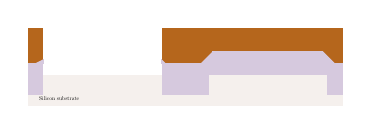
\begin{tikzpicture}[node distance = 3cm, auto, thick,scale=\CrossAndTopSection, every node/.style={transform shape}]
		% resist
\fill[resist] (0,2.6) rectangle (1,5.0);
\fill[resist] (8.5,2.6) rectangle (20,5.0);

% oxide
\fill[isolationoxide] (0,1.25) rectangle (1,2.75);
\fill[isolationoxide] (8.5,1.25) rectangle (20,2.75);

% oxide hill 1
\filldraw[line width=0, isolationoxide] (0.5,2.75) -- (1.0,2.75) -- (1.0,3.0);
\filldraw[line width=0, isolationoxide] (8.75,2.75) -- (8.5,2.75) -- (8.5,3.0);

% oxide hill 2
\fill[isolationoxide] (11.75,2.75) rectangle (18.75,3.5);
\filldraw[line width=0, isolationoxide] (11.0,2.75) -- (11.75,2.75) -- (11.75,3.5);
\filldraw[line width=0, isolationoxide] (18.75,2.75) -- (18.75,3.5) -- (19.5,2.75);

% substrate
\fill[substrate] (0,0) rectangle (20,2);
\node at (2,0.5) {Silicon substrate};
%trenches
\fill[isolationoxide] (0,0.75) rectangle (1,2);
\fill[isolationoxide] (8.5,0.75) rectangle (11.5,2);
\fill[isolationoxide] (19,0.75) rectangle (20,2);
	\end{tikzpicture}
	
\begin{tikzpicture}[node distance = 3cm, auto, thick,scale=\CrossAndTopSection, every node/.style={transform shape}]
		% resist
\fill[resist] (0,0) rectangle (20,12);
% substrate
\fill[substrate] (1.25,1) rectangle (8.25,7.25);
	\end{tikzpicture}
	\caption{Cross/top view of n-well oxide window}
\end{figure}

Since the silicon dioxide layer is 300nm thick and we wanna reach the silicon below we can use wet etching as described in the chemistry chapter.\\

\textbf{Possible approaches}:
\begin{itemize}
	\item \textbf{"AOE Etcher (DRY-AOE)" from HKUST} \\
	We can use anisotropic plasma etching for sharper borders.
	\item \textbf{Chemical solution} \\
	We can use buffered hydrofluoric acid (BOE (1:6)) at room temperature for a little bit over 3 minutes in order to get through the 300nm of oxide.\\
	Too long over 3 minutes might cause under-etch however!
\end{itemize}

\subsection{Cleaning}
In order to avoid contamination of the machines we need to make sure all the resist has been stripped off from the wafer.
\begin{figure}[H]
	\centering
	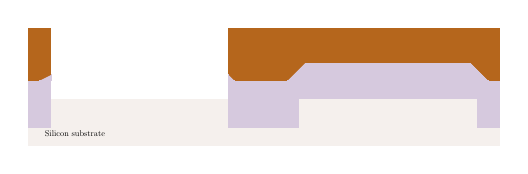
\begin{tikzpicture}[node distance = 3cm, auto, thick,scale=\CrossSectionOnly, every node/.style={transform shape}]
		% resist
\fill[resist] (0,2.6) rectangle (1,5.0);
\fill[resist] (8.5,2.6) rectangle (20,5.0);

% oxide
\fill[isolationoxide] (0,1.25) rectangle (1,2.75);
\fill[isolationoxide] (8.5,1.25) rectangle (20,2.75);

% oxide hill 1
\filldraw[line width=0, isolationoxide] (0.5,2.75) -- (1.0,2.75) -- (1.0,3.0);
\filldraw[line width=0, isolationoxide] (8.75,2.75) -- (8.5,2.75) -- (8.5,3.0);

% oxide hill 2
\fill[isolationoxide] (11.75,2.75) rectangle (18.75,3.5);
\filldraw[line width=0, isolationoxide] (11.0,2.75) -- (11.75,2.75) -- (11.75,3.5);
\filldraw[line width=0, isolationoxide] (18.75,2.75) -- (18.75,3.5) -- (19.5,2.75);

% substrate
\fill[substrate] (0,0) rectangle (20,2);
\node at (2,0.5) {Silicon substrate};
%trenches
\fill[isolationoxide] (0,0.75) rectangle (1,2);
\fill[isolationoxide] (8.5,0.75) rectangle (11.5,2);
\fill[isolationoxide] (19,0.75) rectangle (20,2);
	\end{tikzpicture}
	\drawStepArrow{}
	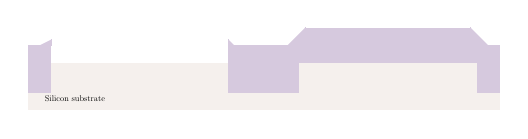
\begin{tikzpicture}[node distance = 3cm, auto, thick,scale=\CrossSectionOnly, every node/.style={transform shape}]
		% oxide
\fill[isolationoxide] (0,1.25) rectangle (1,2.75);
\fill[isolationoxide] (8.5,1.25) rectangle (20,2.75);

% oxide hill 1
\filldraw[line width=0, isolationoxide] (0.5,2.75) -- (1.0,2.75) -- (1.0,3.0);
\filldraw[line width=0, isolationoxide] (8.75,2.75) -- (8.5,2.75) -- (8.5,3.0);

% oxide hill 2
\fill[isolationoxide] (11.75,2.75) rectangle (18.75,3.5);
\filldraw[line width=0, isolationoxide] (11.0,2.75) -- (11.75,2.75) -- (11.75,3.5);
\filldraw[line width=0, isolationoxide] (18.75,2.75) -- (18.75,3.5) -- (19.5,2.75);

% substrate
\fill[substrate] (0,0) rectangle (20,2);
\node at (2,0.5) {Silicon substrate};
%trenches
\fill[isolationoxide] (0,0.75) rectangle (1,2);
\fill[isolationoxide] (8.5,0.75) rectangle (11.5,2);
\fill[isolationoxide] (19,0.75) rectangle (20,2);
	\end{tikzpicture}
	\caption{Resist removal}
\end{figure}
Please just use the solvent for the specific resist.

\newpage

\subsection{Implantation/Doping}\label{nwell_implant_step}
We now need to inject the carriers into the upper level of the n-channel area so that we can later on drive them into the crystal during the drive-in step.

\begin{figure}[H]
	\centering
	\begin{minipage}{0.5\textwidth}
	\centering
	\begin{tikzpicture}[node distance = 3cm, auto, thick,scale=\CrossSectionOnly, every node/.style={transform shape}]
		% oxide
\fill[isolationoxide] (0,1.25) rectangle (1,2.75);
\fill[isolationoxide] (8.5,1.25) rectangle (20,2.75);

% oxide hill 1
\filldraw[line width=0, isolationoxide] (0.5,2.75) -- (1.0,2.75) -- (1.0,3.0);
\filldraw[line width=0, isolationoxide] (8.75,2.75) -- (8.5,2.75) -- (8.5,3.0);

% oxide hill 2
\fill[isolationoxide] (11.75,2.75) rectangle (18.75,3.5);
\filldraw[line width=0, isolationoxide] (11.0,2.75) -- (11.75,2.75) -- (11.75,3.5);
\filldraw[line width=0, isolationoxide] (18.75,2.75) -- (18.75,3.5) -- (19.5,2.75);

\input{tikz_process_steps/sti.a.tex}

\forloop{ct}{0}{\value{ct} < 21}
{
	\draw [->] (\value{ct},5) -- (\value{ct},4);
	\node at (\value{ct},5.2) {P$^{31}$};
}
	\end{tikzpicture}
	\drawStepArrow{Boron implant}
	\begin{tikzpicture}[node distance = 3cm, auto, thick,scale=\CrossSectionOnly, every node/.style={transform shape}]
		% resist
\fill[resist] (0.25,2.0) rectangle (1,5.0);
\fill[resist] (8.5,2.0) rectangle (19.75,5.0);

% oxide
\fill[isolationoxide] (0,1.25) rectangle (1,2.75);
\fill[isolationoxide] (8.5,1.25) rectangle (20,2.75);

% oxide hill 1
\filldraw[line width=0, isolationoxide] (0.5,2.75) -- (1.0,2.75) -- (1.0,3.0);
\filldraw[line width=0, isolationoxide] (8.75,2.75) -- (8.5,2.75) -- (8.5,3.0);

% oxide hill 2
\fill[isolationoxide] (11.75,2.75) rectangle (18.75,3.5);
\filldraw[line width=0, isolationoxide] (11.0,2.75) -- (11.75,2.75) -- (11.75,3.5);
\filldraw[line width=0, isolationoxide] (18.75,2.75) -- (18.75,3.5) -- (19.5,2.75);

\input{tikz_process_steps/sti.a.tex}

	\end{tikzpicture}
	\drawStepArrow{Annealing}
	\begin{tikzpicture}[node distance = 3cm, auto, thick,scale=\CrossSectionOnly, every node/.style={transform shape}]
		% oxide
\fill[isolationoxide] (0,1.25) rectangle (1,2.75);
\fill[isolationoxide] (8.5,1.25) rectangle (20,2.75);

% oxide hill 1
\filldraw[line width=0, isolationoxide] (0.5,2.75) -- (1.0,2.75) -- (1.0,3.0);
\filldraw[line width=0, isolationoxide] (8.75,2.75) -- (8.5,2.75) -- (8.5,3.0);

% oxide hill 2
\fill[isolationoxide] (11.75,2.75) rectangle (18.75,3.5);
\filldraw[line width=0, isolationoxide] (11.0,2.75) -- (11.75,2.75) -- (11.75,3.5);
\filldraw[line width=0, isolationoxide] (18.75,2.75) -- (18.75,3.5) -- (19.5,2.75);

\input{tikz_process_steps/sti.a.tex}
\shade[upper left = nwell, upper right = nwell, lower right = substrate, lower left = substrate,] (1.25,1.5) rectangle (8.25,2.0);
\shade[upper left = pwell, upper right = pwell, lower right = substrate, lower left = substrate,] (11.75,1.0) rectangle (18.75,2.0);
	\end{tikzpicture} \\
	\textbf{Implantation approach}
	\end{minipage}\begin{minipage}{0.5\textwidth}
	\centering
	\begin{tikzpicture}[node distance = 3cm, auto, thick,scale=\CrossSectionOnly, every node/.style={transform shape}]
		\fill[nwell] (0,0) rectangle (20,5);

% oxide
\fill[isolationoxide] (0,1.25) rectangle (1,2.75);
\fill[isolationoxide] (8.5,1.25) rectangle (20,2.75);

% oxide hill 1
\filldraw[line width=0, isolationoxide] (0.5,2.75) -- (1.0,2.75) -- (1.0,3.0);
\filldraw[line width=0, isolationoxide] (8.75,2.75) -- (8.5,2.75) -- (8.5,3.0);

% oxide hill 2
\fill[isolationoxide] (11.75,2.75) rectangle (18.75,3.5);
\filldraw[line width=0, isolationoxide] (11.0,2.75) -- (11.75,2.75) -- (11.75,3.5);
\filldraw[line width=0, isolationoxide] (18.75,2.75) -- (18.75,3.5) -- (19.5,2.75);

\input{tikz_process_steps/sti.a.tex}
	\end{tikzpicture}
	\drawStepArrow{Constant source diffusion}
	\begin{tikzpicture}[node distance = 3cm, auto, thick,scale=\CrossSectionOnly, every node/.style={transform shape}]
		\fill[nwell] (0,0) rectangle (20,5);

% oxide
\fill[isolationoxide] (0,1.25) rectangle (1,2.75);
\fill[isolationoxide] (8.5,1.25) rectangle (20,2.75);

% oxide hill 1
\filldraw[line width=0, isolationoxide] (0.5,2.75) -- (1.0,2.75) -- (1.0,3.0);
\filldraw[line width=0, isolationoxide] (8.75,2.75) -- (8.5,2.75) -- (8.5,3.0);

% oxide hill 2
\fill[isolationoxide] (11.75,2.75) rectangle (18.75,3.5);
\filldraw[line width=0, isolationoxide] (11.0,2.75) -- (11.75,2.75) -- (11.75,3.5);
\filldraw[line width=0, isolationoxide] (18.75,2.75) -- (18.75,3.5) -- (19.5,2.75);

\input{tikz_process_steps/sti.a.tex}

\shade[upper left = nwell, upper right = nwell, lower right = substrate, lower left = substrate,] (1.25,1.5) rectangle (8.25,2.0);
\shade[upper left = pwell, upper right = pwell, lower right = substrate, lower left = substrate,] (11.75,1.0) rectangle (18.75,2.0);
	\end{tikzpicture}
	\drawStepArrow{Source removal}
	\begin{tikzpicture}[node distance = 3cm, auto, thick,scale=\CrossSectionOnly, every node/.style={transform shape}]
		% oxide
\fill[isolationoxide] (0,1.25) rectangle (1,2.75);
\fill[isolationoxide] (8.5,1.25) rectangle (20,2.75);

% oxide hill 1
\filldraw[line width=0, isolationoxide] (0.5,2.75) -- (1.0,2.75) -- (1.0,3.0);
\filldraw[line width=0, isolationoxide] (8.75,2.75) -- (8.5,2.75) -- (8.5,3.0);

% oxide hill 2
\fill[isolationoxide] (11.75,2.75) rectangle (18.75,3.5);
\filldraw[line width=0, isolationoxide] (11.0,2.75) -- (11.75,2.75) -- (11.75,3.5);
\filldraw[line width=0, isolationoxide] (18.75,2.75) -- (18.75,3.5) -- (19.5,2.75);

\input{tikz_process_steps/sti.a.tex}

\shade[upper left = nwell, upper right = nwell, lower right = substrate, lower left = substrate,] (1.25,1.5) rectangle (8.25,2.0);
\shade[upper left = pwell, upper right = pwell, lower right = substrate, lower left = substrate,] (11.75,1.0) rectangle (18.75,2.0);
	\end{tikzpicture} \\
	\textbf{Diffusion approach}
	\end{minipage}
	\caption{Doping process}
\end{figure}


\textbf{Possible approaches}:
\begin{itemize}
	\item \textbf{"CF-3000 Implanter (IMP-3000)" from HKUST} \\
	At HKUST we have an implanter which gives us better control over the initial surface concentration. \\
	These steps are needed to arrive with the desired geometry:
	\begin{enumerate}
		\item Preparing by default cleaning
		\item The N-well is implanted with a Phosphorus ($P^{31}$) dose of $2.5\times10^{12}cm^{-2}$ at an energy of 100 keV.
		\item The N-well is annealed for 30 minutes at 1050\degreesC in $N_2$ environment (DIF-A1)\\
		After that the P-well will be around 2\um deep and the N-Well around 1\um deep
	\end{enumerate}
	\item \textbf{Constant source diffusion} \\
	We can add a layer of Phosphorus solution and diffusing in order to have an initial concentration in order to reach the desired concentration later by main diffusion.
		\begin{enumerate}
		\item A constant source is added (gas or liquid)
		\item The source dopant is driven in for 10 minutes at 1050\degreesC
		\item The dopant source is removed by stopping the gas flow or cleaning the surface
	\end{enumerate}
\end{itemize}

\newpage

\subsection{Oxide for drive-in}

Now we need to cover the now doped and annealed area with an oxide layer in order to seal it off and prevent the dopants from diffusing out of the crystal during the drive-in phase.

\begin{figure}[H]
	\centering
	\begin{tikzpicture}[node distance = 3cm, auto, thick,scale=\CrossSectionOnly, every node/.style={transform shape}]
		% resist
\fill[resist] (0.25,2.0) rectangle (1,5.0);
\fill[resist] (8.5,2.0) rectangle (19.75,5.0);

\input{tikz_process_steps/nwell.cleaning.b.tex}

	\end{tikzpicture}
	\drawStepArrow{}
	\begin{tikzpicture}[node distance = 3cm, auto, thick,scale=\CrossSectionOnly, every node/.style={transform shape}]
		\fill[isolationoxide] (0,0) rectangle (20,2.25);
\input{tikz_process_steps/nwell.cleaning.b.tex}
\shade[upper left = nwell, upper right = nwell, lower right = substrate, lower left = substrate,] (1.25,1.5) rectangle (8.25,2.0);
\shade[upper left = pwell, upper right = pwell, lower right = substrate, lower left = substrate,] (11.75,1.0) rectangle (18.75,2.0);
	\end{tikzpicture}
	\caption{Oxide growth}
\end{figure}

The wafer is being oxidized for around 5 minutes at 1050\degree C in a wet environment in order to achieve a cover silicon layer of around 90nm thickness.

\subsection{Drive-in}
In order to drive the carrier atoms deeper into the crystalline structure the wafer needs to be driven in after predeposition.

\begin{figure}[H]
	\centering
	\begin{tikzpicture}[node distance = 3cm, auto, thick,scale=\CrossSectionOnly, every node/.style={transform shape}]
		\fill[isolationoxide] (0,0) rectangle (20,2.25);
\input{tikz_process_steps/nwell.implantation.c.tex}
	\end{tikzpicture}
	\drawStepArrow{}
	\begin{tikzpicture}[node distance = 3cm, auto, thick,scale=\CrossSectionOnly, every node/.style={transform shape}]
		\fill[isolationoxide] (0,0) rectangle (20,2.25);
% resist
\fill[resist] (0.25,2.0) rectangle (1,5.0);
\fill[resist] (8.5,2.0) rectangle (19.75,5.0);

\input{tikz_process_steps/nwell.cleaning.b.tex}


% n-well
\fill[nwell] (1.25,0.75) rectangle (8.25,2);
\node at (4.75,1) {N-Well};

\fill[pwell] (11.75,0.75) rectangle (18.75,2);
\node at (15.25,1) {P-Well};
	\end{tikzpicture}
	\caption{Drive-in process}
\end{figure}

In this step the wafer is  driven-in for 90 minutes at 1050\degree C in an inert ambient\footnote{\url{http://cleanroom.byu.edu/DopConCalc}}

\subsection{Oxide mask removal}
Now we want to remove the silicon mask from the wafer and clean it for another clean oxide mask layer.

\begin{figure}[H]
	\centering
	\begin{tikzpicture}[node distance = 3cm, auto, thick,scale=\CrossSectionOnly, every node/.style={transform shape}]
		\fill[isolationoxide] (0,0) rectangle (20,2.25);
% resist
\fill[resist] (0.25,2.0) rectangle (1,5.0);
\fill[resist] (8.5,2.0) rectangle (19.75,5.0);

\input{tikz_process_steps/nwell.cleaning.b.tex}


% n-well
\fill[nwell] (1.25,0.75) rectangle (8.25,2);
\node at (4.75,1) {N-Well};

\fill[pwell] (11.75,0.75) rectangle (18.75,2);
\node at (15.25,1) {P-Well};
	\end{tikzpicture}
	\drawStepArrow{}
	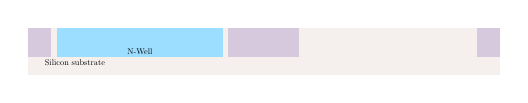
\begin{tikzpicture}[node distance = 3cm, auto, thick,scale=\CrossSectionOnly, every node/.style={transform shape}]
		% substrate
\fill[substrate] (0,0) rectangle (20,2);
\node at (2,0.5) {Silicon substrate};
%trenches
\fill[isolationoxide] (0,0.75) rectangle (1,2);
\fill[isolationoxide] (8.5,0.75) rectangle (11.5,2);
\fill[isolationoxide] (19,0.75) rectangle (20,2);

% n-well
\fill[nwell] (1.25,0.75) rectangle (8.25,2);
\node at (4.75,1) {N-Well};
	\end{tikzpicture}
	\caption{Oxide removal}
\end{figure}

We use buffered hydrofluoric acid (BOE (1:6)) at room temperature for 3 minutes in order to remove the 300nm of oxide layer.
\newpage
`\section{P-well}\label{pwell_chapter}
In order to build CMOS on the same substrate, a P-well is required for building the complementary N-channel transistor for a n-p-channel logic circuitry.
The cross section as well as the top view of the targeted geometry are shown in \autoref{nwell_target}
\begin{figure}[H]
	\centering
	\begin{tikzpicture}[node distance = 3cm, auto, thick,scale=\CrossAndTopSectionBig, every node/.style={transform shape}]
		\input{tikz_process_steps/sti.a.tex}
% n-well
\fill[nwell] (1.25,0.75) rectangle (8.5,2);
\node at (5.75,1) {N-Well};


% p-well
\fill[pwell] (11.75,0.75) rectangle (18.75,2);
\node at (14.25,1) {P-Well};
	\end{tikzpicture}
	\begin{tikzpicture}[node distance = 3cm, auto, thick,scale=\CrossAndTopSectionBig, every node/.style={transform shape}]
		\input{tikz_process_steps/sti.b.tex}
\fill[nwell] (1.25,1) rectangle (8.25,7.25);
\fill[pwell] (11.75,1) rectangle (18.75,7.25);
	\end{tikzpicture}
	\caption{P-well target geometry}
	\label{pwell_target}
\end{figure}
The P-well will serve us as an island of higher p-doped substrate within the slightly p-doped basis substrate.

The dopant dose will be $2.5\times10^{12}cm^{-2}$ as calculated in the documentation of the process design leading to these steps\footnote{\url{https://github.com/leviathanch/libresiliconprocess/raw/master/process_design/process_design.pdf}}.

\begin{figure}[H]
	\centering
	\begin{tikzpicture}[node distance =1cm, auto, thick,scale=\VLSILayout, every node/.style={transform shape}]
		\input{tikz_process_steps/sti.layout.tex}
\fill[nwell,opacity=\OpacityLayout] (1,0.75) rectangle (8.5,7.5);
\fill[pwell,opacity=\OpacityLayout] (11.5,0.75) rectangle (19,7.5);
	\end{tikzpicture}
	\caption{P-Well layout}
	\label{pwell_layout}
\end{figure}

In \autoref{pwell_layout} the layout of the P-well region on top of the active area region can be seen.

The p-well is being fit into the active area.

It should even be a little bit bigger than the active area, because of possible alignment offsets

\newpage

\subsection{Mask dioxide layer}
In order to selectively inject charge carrying atoms into the crystalline structure a protective dioxide ($SiO_2$) layer needs to be grown on top of a p-type substrate.
\begin{figure}[H]
	\centering
	\begin{tikzpicture}[node distance = 3cm, auto, thick,scale=\CrossSectionOnly, every node/.style={transform shape}]
		\input{tikz_process_steps/sti.a.tex}
% n-well
\fill[nwell] (1.25,0.75) rectangle (8.5,2);
\node at (5.75,1) {N-Well};


	\end{tikzpicture} \\
	
\includegraphics[scale=0.01]{down_arrow.png} \\
	\begin{tikzpicture}[node distance = 3cm, auto, thick,scale=\CrossSectionOnly, every node/.style={transform shape}]
		% oxide
\fill[isolationoxide] (0,1.25) rectangle (20,2.75);

% oxide hill 1
\fill[isolationoxide] (1.25,2.75) rectangle (8.25,3.5);
\filldraw[line width=0, isolationoxide] (0.5,2.75) -- (1.25,2.75) -- (1.25,3.5);
\filldraw[line width=0, isolationoxide] (8.25,2.75) -- (8.25,3.5) -- (9.0,2.75);

% oxide hill 2
\fill[isolationoxide] (11.75,2.75) rectangle (18.75,3.5);
\filldraw[line width=0, isolationoxide] (11.0,2.75) -- (11.75,2.75) -- (11.75,3.5);
\filldraw[line width=0, isolationoxide] (18.75,2.75) -- (18.75,3.5) -- (19.5,2.75);

\node at (2,2.1) {SiO2};

\input{tikz_process_steps/nwell.a.tex}
	\end{tikzpicture}
	\caption{Dioxide layer growth}
\end{figure}
With an energy of 100keV for the implantation performed in \autoref{pwell_implant_step}, the projected range of the dopants within the oxide will be 310nm (380nm tops) \footnote{\url{http://cleanroom.byu.edu/rangestraggle}}.
This means being on the safe side and having 500nm as the thickness is a good approach.

In order to grow the 500nm thick oxide layer, the wafer is being oxidized for around 56 minutes at 1050\degree C using wet oxidation which results in a dioxide layer of around 500nm in thickness\footnote{\url{http://cleanroom.byu.edu/OxideTimeCalc}}.

\subsection{Patterning}
The resist is being deposited spray or spin coating (spray coating is better because of the uneven surface!) and then soft baked depending on the baking time for the specific resist.
The layout for being exposed onto the resist is being extracted from the "pwell" layer within the GDS2 file onto a \textbf{bright field} mask.
The requirement is a \textbf{negative} tone resist.

\begin{figure}[H]
	\centering
	\begin{tikzpicture}[node distance = 3cm, auto, thick,scale=\CrossAndTopSection, every node/.style={transform shape}]
		% oxide
\fill[isolationoxide] (0,1.25) rectangle (20,2.75);

% oxide hill 1
\fill[isolationoxide] (1.25,2.75) rectangle (8.25,3.5);
\filldraw[line width=0, isolationoxide] (0.5,2.75) -- (1.25,2.75) -- (1.25,3.5);
\filldraw[line width=0, isolationoxide] (8.25,2.75) -- (8.25,3.5) -- (9.0,2.75);

% oxide hill 2
\fill[isolationoxide] (11.75,2.75) rectangle (18.75,3.5);
\filldraw[line width=0, isolationoxide] (11.0,2.75) -- (11.75,2.75) -- (11.75,3.5);
\filldraw[line width=0, isolationoxide] (18.75,2.75) -- (18.75,3.5) -- (19.5,2.75);

\node at (2,2.1) {SiO2};

\input{tikz_process_steps/pwell.mask_dioxide_layer.a.tex}
	\end{tikzpicture}
	\begin{tikzpicture}[node distance = 3cm, auto, thick,scale=\CrossAndTopSection, every node/.style={transform shape}]
		% resist
\fill[isolationoxide] (0,0) rectangle (20,12);
	\end{tikzpicture} \\
	
\includegraphics[scale=0.01]{down_arrow.png} \\
	\begin{tikzpicture}[node distance = 3cm, auto, thick,scale=\CrossAndTopSection, every node/.style={transform shape}]
		% resist
\fill[resist] (0.25,2.0) rectangle (11.5,5.0);
\fill[resist] (19,2.0) rectangle (19.75,5.0);

\input{tikz_process_steps/pwell.mask_dioxide_layer.b.tex}

	\end{tikzpicture}
	\begin{tikzpicture}[node distance = 3cm, auto, thick,scale=\CrossAndTopSection, every node/.style={transform shape}]
		% resist
\fill[resist] (0,0) rectangle (20,12);
% substrate
\fill[isolationoxide] (11.5,1.5) rectangle (19,7.25);
	\end{tikzpicture}
	\caption{Cross/top view of P-well layout on resist}
\end{figure}
The thickness of the resist layer and the baking duration will variate depending on the specific equipment for which this process will be implemented with.
Also after the exposure and development, the hard baking shouldn't be forgotten!

\newpage

\subsection{Etching}
We now need to open a window in the dioxide layer, through which we will inject carrier atoms into the silicon crystal structure.
\begin{figure}[H]
	\centering
	\begin{tikzpicture}[node distance = 3cm, auto, thick,scale=\CrossAndTopSection, every node/.style={transform shape}]
		% resist
\fill[resist] (0.25,2.0) rectangle (11.5,5.0);
\fill[resist] (19,2.0) rectangle (19.75,5.0);

\input{tikz_process_steps/pwell.patterning.a.tex}

	\end{tikzpicture}
	\begin{tikzpicture}[node distance = 3cm, auto, thick,scale=\CrossAndTopSection, every node/.style={transform shape}]
		% resist
\fill[resist] (0,0) rectangle (20,12);
% substrate
\fill[isolationoxide] (1.25,1.5) rectangle (8.25,7.25);
	\end{tikzpicture} \\
	
\includegraphics[scale=0.01]{down_arrow.png} \\
	\begin{tikzpicture}[node distance = 3cm, auto, thick,scale=\CrossAndTopSection, every node/.style={transform shape}]
		% resist
\fill[resist] (0,2.6) rectangle (11.5,5.0);
\fill[resist] (19,2.6) rectangle (20,5.0);

% oxide
\fill[isolationoxide] (0,1.25) rectangle (11.5,2.75);
\fill[isolationoxide] (19,1.25) rectangle (20,2.75);

% oxide hill 1
\fill[isolationoxide] (1.25,2.75) rectangle (8.25,3.5);
\filldraw[line width=0, isolationoxide] (0.5,2.75) -- (1.25,2.75) -- (1.25,3.5);
\filldraw[line width=0, isolationoxide] (8.25,2.75) -- (8.25,3.5) -- (9.0,2.75);

% oxide hill 2
\filldraw[line width=0, isolationoxide] (11.25,2.75) -- (11.5,2.75) -- (11.5,3.0);
\filldraw[line width=0, isolationoxide] (19.0,3.0)  -- (19.0,2.75) -- (19.00,2.75);

\node at (2,2.1) {SiO2};

\input{tikz_process_steps/nwell.a.tex}


	\end{tikzpicture}
	\begin{tikzpicture}[node distance = 3cm, auto, thick,scale=\CrossAndTopSection, every node/.style={transform shape}]
		% resist
\fill[resist] (0,0) rectangle (20,12);
% substrate
\fill[substrate] (1.25,1.5) rectangle (8.25,7.25);
	\end{tikzpicture}
	\caption{Cross/top view of P-well oxide window}
\end{figure}

There are multiple possible approaches to etch through these 500nm of oxide.\\

\textbf{Possible approaches}:
\begin{itemize}
	\item \textbf{"AOE Etcher (DRY-AOE)" from HKUST} \\
	We can use anisotropic plasma etching for sharper borders.
	\item \textbf{Chemical solution} \\
	We can use buffered hydrofluoric acid (BOE (1:6)) at room temperature for 5 minutes in order to get through the 500nm of oxide.\\
	Too long over 4 minutes might cause under-etch however!
\end{itemize}

\subsection{Cleaning}
In order to avoid contamination of the machines we need to make sure all the resist has been stripped off from the wafer.
\begin{figure}[H]
	\centering
	\begin{tikzpicture}[node distance = 3cm, auto, thick,scale=\CrossSectionOnly, every node/.style={transform shape}]
		\input{tikz_process_steps/pwell.patterning.b.tex}

% boron
\shade[upper left = pwell, upper right = pwell, lower right = substrate, lower left = substrate,] (11.5,1.5) rectangle (19.0,2);


	\end{tikzpicture} \\
	
\includegraphics[scale=0.01]{down_arrow.png} \\
	\begin{tikzpicture}[node distance = 3cm, auto, thick,scale=\CrossSectionOnly, every node/.style={transform shape}]
		% substrate
\fill[substrate] (0,0) rectangle (20,1.25);
\node at (2,0.5) {Silicon substrate};
\fill[substrate] (0.25,1.25) rectangle (19.75,2);

% boron
\shade[upper left = pwell, upper right = pwell, lower right = substrate, lower left = substrate,] (11.5,1.5) rectangle (19.0,2);

	\end{tikzpicture}
	\caption{Resist removal}
\end{figure}
Please just use the solvent for the specific resist.

\newpage

\subsection{Implantation/Predeposition}\label{pwell_implant_step}
We now need to inject the carriers into the upper level of the n-channel area so that we can later on drive them into the crystal during the drive-in step.
\begin{figure}[H]
	\centering
	\begin{tikzpicture}[node distance = 3cm, auto, thick,scale=\CrossSectionOnly, every node/.style={transform shape}]
		% oxide
\fill[isolationoxide] (0,1.25) rectangle (11.5,2.75);
\fill[isolationoxide] (19,1.25) rectangle (20,2.75);

% oxide hill 1
\fill[isolationoxide] (1.25,2.75) rectangle (8.25,3.5);
\filldraw[line width=0, isolationoxide] (0.5,2.75) -- (1.25,2.75) -- (1.25,3.5);
\filldraw[line width=0, isolationoxide] (8.25,2.75) -- (8.25,3.5) -- (9.0,2.75);

% oxide hill 2
\filldraw[line width=0, isolationoxide] (11.25,2.75) -- (11.5,2.75) -- (11.5,3.0);
\filldraw[line width=0, isolationoxide] (19.0,3.0)  -- (19.0,2.75) -- (19.25,2.75);

\node at (2,2.1) {SiO2};

\input{tikz_process_steps/nwell.a.tex}

\forloop{ct}{0}{\value{ct} < 21}
{
	\draw [->] (\value{ct},5) -- (\value{ct},4);
	\node at (\value{ct},5.2) {P$^{31}$};
}
	\end{tikzpicture} \\
	
\includegraphics[scale=0.01]{down_arrow.png} \\
	\begin{tikzpicture}[node distance = 3cm, auto, thick,scale=\CrossSectionOnly, every node/.style={transform shape}]
		% resist
\fill[resist] (0.25,2.0) rectangle (11.5,5.0);
\fill[resist] (19,2.0) rectangle (19.75,5.0);

\input{tikz_process_steps/pwell.patterning.a.tex}


% boron
\shade[upper left = pwell, upper right = pwell, lower right = substrate, lower left = substrate,] (11.5,1.5) rectangle (19.0,2);

	\end{tikzpicture} \\
	
\includegraphics[scale=0.01]{down_arrow.png} \\
	\begin{tikzpicture}[node distance = 3cm, auto, thick,scale=\CrossSectionOnly, every node/.style={transform shape}]
		% oxide
\fill[isolationoxide] (0,1.25) rectangle (11.5,2.75);
\fill[isolationoxide] (19,1.25) rectangle (20,2.75);

% oxide hill 1
\fill[isolationoxide] (1.25,2.75) rectangle (8.25,3.5);
\filldraw[line width=0, isolationoxide] (0.5,2.75) -- (1.25,2.75) -- (1.25,3.5);
\filldraw[line width=0, isolationoxide] (8.25,2.75) -- (8.25,3.5) -- (9.0,2.75);

% oxide hill 2
\filldraw[line width=0, isolationoxide] (11.25,2.75) -- (11.5,2.75) -- (11.5,3.0);
\filldraw[line width=0, isolationoxide] (19.0,3.0)  -- (19.0,2.75) -- (19.25,2.75);

\node at (2,2.1) {SiO2};

\input{tikz_process_steps/nwell.a.tex}

% boron
\fill[pwell] (11.75,1.5) rectangle (18.75,2);
	\end{tikzpicture}
	\caption{Doping process}
\end{figure}

\textbf{Possible approaches}:
\begin{itemize}
	\item \textbf{"CF-3000 Implanter (IMP-3000)" from HKUST} \\
	At HKUST we have an implanter which gives us better control over the initial surface concentration. \\
	These steps are needed to arrive with the desired geometry:
	\begin{enumerate}
		\item Preparing by default cleaning
		\item The P-well is implanted with a Boron ($B^{11}$) dose of $2.5\times10^{12}cm^{-2}$ at an energy of 100 keV
		\item The P-well is annealed for 30 minutes at 1050\degreesC in $N_2$ environment (DIF-A1)\\
		After that the P-well will be around 1\um deep (and will become deeper during \autoref{nwell_implant_step})
	\end{enumerate}
	\item \textbf{Constant source diffusion} \\
	We can add a layer of Boron solution and diffusing in order to have an initial concentration in order to reach the desired concentration later by main diffusion.
\end{itemize}

\subsection{Oxide mask removal}
Now we want to remove the silicon mask from the wafer and clean it for another clean oxide mask layer in order to perform the implantation of the N-well in the next step.

\begin{figure}[H]
	\centering
	\begin{tikzpicture}[node distance = 3cm, auto, thick,scale=\CrossSectionOnly, every node/.style={transform shape}]
		\input{tikz_process_steps/nwell.a.tex}

% boron
\fill[pwell] (11.5,1.8) rectangle (19,2);
\fill[pwell] (0,2.5) rectangle (11.5,2.6);
\fill[pwell] (19,2.5) rectangle (20,2.6);

% oxide
\fill[isolationoxide] (0,2) rectangle (11.5,2.6);
\fill[isolationoxide] (19,2) rectangle (20,2.6);
\fill[isolationoxide] (1.5,2) rectangle (19,2.3); % cover

% pwell
\fill[pwell] (11.75,0.75) rectangle (18.75,2);
	\end{tikzpicture} \\
	
\includegraphics[scale=0.01]{down_arrow.png} \\
	\begin{tikzpicture}[node distance = 3cm, auto, thick,scale=\CrossSectionOnly, every node/.style={transform shape}]
		\input{tikz_process_steps/nwell.a.tex}

% pwell
\fill[pwell] (11.75,0.75) rectangle (18.75,2);
\node at (14.25,1) {P-Well};
	\end{tikzpicture}
	\caption{Oxide removal}
\end{figure}

We use buffered hydrofluoric acid (BOE (1:6)) at room temperature for 5 minutes in order to remove the 500nm of oxide layer.
\newpage
\section{Gate}\label{gate}
Now we have to build the initial gate structure which contains of the 40nm thick dielectric (in our case just silicon dioxide) and the polysilicon electrode.

\begin{figure}[H]
	\centering
	\begin{tikzpicture}[node distance = 3cm, auto, thick,scale=\CrossAndTopSectionBig, every node/.style={transform shape}]
		\input{tikz_process_steps/nimplant.a.tex}
\fill[pimplant] (3.0,1.5) rectangle (5,2);
\node at (4,1.65) {p+};
\fill[pimplant] (6.5,1.5) rectangle (8.5,2);
\node at (7,1.65) {p+};
\fill[pimplant] (17,1.5) rectangle (18.75,2);
\node at (18,1.65) {p+};
\fill[gateoxide] (4.8,2) rectangle (6.7,2.3);
\fill[gateoxide] (13.3,2) rectangle (15.2,2.3);
\fill[gatemetal] (4.8,2.3) rectangle (6.7,2.6);
\fill[gatemetal] (13.3,2.3) rectangle (15.2,2.6);
		\node at (3,3) {Gate oxide};
		\draw[->] (3,2.8) -- (5,2.2);
		\node at (3,4) {Polysilicon};
		\draw[->] (3,3.8) -- (5,3.2);
	\end{tikzpicture}
	\begin{tikzpicture}[node distance = 3cm, auto, thick,scale=\CrossAndTopSectionBig, every node/.style={transform shape}]
		\fill[substrate] (0,0) rectangle (20,10);

% n-well
\fill[nwell] (1,1.25) rectangle (8.5,7.5);

% p+
\fill[pimplant] (3.5,2) rectangle (5,6.5);
\fill[pimplant] (6.5,2) rectangle (8,6.5);
\fill[pimplant] (17,2) rectangle (18.5,6.5);

% n+
\fill[nimplant] (1.5,2) rectangle (3,6.5);
\fill[nimplant] (12,2) rectangle (13.5,6.5);
\fill[nimplant] (15,2) rectangle (16.5,6.5);

% trench area
\fill[isolationoxide] (0,0) rectangle (1,12);
\fill[isolationoxide] (8.5,0) rectangle (11.5,12);
\fill[isolationoxide] (19,0) rectangle (20,12);
\fill[isolationoxide] (0,0) rectangle (20,1.25);
\fill[isolationoxide] (0,7.5) rectangle (20,12);

% gate metal
\fill[gatemetal] (4.8,1.75) rectangle (6.7,9);
\fill[gatemetal] (13.3,1.75) rectangle (15.2,9);
\fill[gatemetal] (4.8,8) rectangle (15.2,9);
	\end{tikzpicture}
	\caption{Aluminum gate contacts with gate oxide}
\end{figure}

The line spacing of the polysilicon electrode shape has to be at least 0.5\um because of the resolution of the stepper and also because of the etching process which has 0.5\um as the minimum line spacing.

\begin{figure}[H]
	\centering
	\begin{tikzpicture}[node distance =1cm, auto, thick,scale=\VLSILayout, every node/.style={transform shape}]
		\input{tikz_process_steps/nimplant.layout.tex}

% p+
\fill[pimplant,opacity=\OpacityLayout] (3,0.75) rectangle (8.5,7.5);
\fill[pimplant,opacity=\OpacityLayout] (17,0.75) rectangle (19,7.5);
% gate metal
\fill[gatemetal,opacity=\OpacityLayout] (4.8,1.75) rectangle (6.7,8);
\fill[gatemetal,opacity=\OpacityLayout] (13.3,1.75) rectangle (15.2,8);
\fill[gatemetal,opacity=\OpacityLayout] (4.8,8) rectangle (15.2,10);

	\end{tikzpicture}
	\caption{Gate layout}
	\label{gate_layout}
\end{figure}

In \autoref{gate_layout} we can see the layout honoring the 0.5\um spacing design rule for the gate structure shape and poly-layer interconnect between NMOS and PMOS.

\subsection{Gate oxide deposition}

\begin{figure}[H]
	\centering
	\begin{tikzpicture}[node distance = 3cm, auto, thick,scale=\CrossSectionOnly, every node/.style={transform shape}]
		\input{tikz_process_steps/nwell.a.tex}
% p-well
\fill[pwell] (11.75,0.75) rectangle (18.75,2);
\node at (14.25,1) {P-Well};
	\end{tikzpicture} \\
	
\includegraphics[scale=0.01]{down_arrow.png} \\
	\begin{tikzpicture}[node distance = 3cm, auto, thick,scale=\CrossSectionOnly, every node/.style={transform shape}]
		\input{tikz_process_steps/nwell.a.tex}
% p-well
\fill[pwell] (11.75,0.75) rectangle (18.75,2);
\node at (14.25,1) {P-Well};
\fill[gateoxide] (0,2) rectangle (20,2.3);
	\end{tikzpicture}
	\caption{Thin oxide}
\end{figure}

\subsection{Polysilicon deposition}

Now we need to add the polysilicon layer for forming the gate structure after etching.

\begin{figure}[H]
	\centering
	\begin{tikzpicture}[node distance = 3cm, auto, thick,scale=\CrossSectionOnly, every node/.style={transform shape}]
		\input{tikz_process_steps/nwell.a.tex}
% p-well
\fill[pwell] (11.75,0.75) rectangle (18.75,2);
\node at (14.25,1) {P-Well};
\fill[gateoxide] (0,2) rectangle (20,2.3);
	\end{tikzpicture} \\
	
\includegraphics[scale=0.01]{down_arrow.png} \\
	\begin{tikzpicture}[node distance = 3cm, auto, thick,scale=\CrossSectionOnly, every node/.style={transform shape}]
		\input{tikz_process_steps/nwell.a.tex}
% p-well
\fill[pwell] (11.75,0.75) rectangle (18.75,2);
\node at (14.25,1) {P-Well};
\fill[gateoxide] (0,2) rectangle (20,2.3);
\fill[gatemetal] (0,2.3) rectangle (20,3);
	\end{tikzpicture}
	\caption{Polysilicon}
\end{figure}

We use the LPCVD machine(\autoref{lpcvd_machine}) and deposit a layer of around 600nm polysilicon\footnote{\url{https://people.rit.edu/lffeee/LPCVD_Recipes.pdf}}.

We set the temperatue to 650\degreesC, the gas will be Silane ($Si H_4$ ($Si + 2H_2$)), the pressure will be set to 300 mTorr with a flow of 90sccm.

This will give us a growth rate of roughly 23.5 nm per minute, so for 600nm we let it grow half an hour.

\subsection{Patterning}

The resist is being deposited using spin coating and then baked depending on the baking time for the specific resist.
The layout for being exposed onto the resist is being extracted from the "poly" layer within the GDS2 file onto a bright field mask.

\begin{figure}[H]
	\centering
	\begin{tikzpicture}[node distance = 3cm, auto, thick,scale=\CrossSectionOnly, every node/.style={transform shape}]
		\input{tikz_process_steps/nwell.a.tex}
% p-well
\fill[pwell] (11.75,0.75) rectangle (18.75,2);
\node at (14.25,1) {P-Well};
\fill[gateoxide] (0,2) rectangle (20,2.3);
\fill[gatemetal] (0,2.3) rectangle (20,3);
	\end{tikzpicture} \\
	
\includegraphics[scale=0.01]{down_arrow.png} \\
	\begin{tikzpicture}[node distance = 3cm, auto, thick,scale=\CrossSectionOnly, every node/.style={transform shape}]
		\input{tikz_process_steps/nwell.a.tex}
% p-well
\fill[pwell] (11.75,0.75) rectangle (18.75,2);
\node at (14.25,1) {P-Well};
\fill[gateoxide] (0,2) rectangle (20,2.3);
\fill[poly] (0,2.3) rectangle (20,3);

\fill[resist] (5,3) rectangle (6.5,3.6);
\fill[resist] (13.5,3) rectangle (15,3.6);
	\end{tikzpicture}
	\caption{Resist}
\end{figure}

\subsection{Etching}

\begin{figure}[H]
	\centering
	\begin{tikzpicture}[node distance = 3cm, auto, thick,scale=\CrossSectionOnly, every node/.style={transform shape}]
		\input{tikz_process_steps/nwell.a.tex}
% p-well
\fill[pwell] (11.75,0.75) rectangle (18.75,2);
\node at (14.25,1) {P-Well};
\fill[gateoxide] (0,2) rectangle (20,2.3);
\fill[poly] (0,2.3) rectangle (20,3);
\fill[resist] (5,3) rectangle (6.5,3.6);
\fill[resist] (13.5,3) rectangle (15,3.6);
	\end{tikzpicture} \\
	
\includegraphics[scale=0.01]{down_arrow.png} \\
	\begin{tikzpicture}[node distance = 3cm, auto, thick,scale=\CrossSectionOnly, every node/.style={transform shape}]
		\input{tikz_process_steps/nwell.a.tex}
% p-well
\fill[pwell] (11.75,0.75) rectangle (18.75,2);
\node at (14.25,1) {P-Well};
\fill[gateoxide] (5,2) rectangle (6.5,2.3);
\fill[gateoxide] (13.5,2) rectangle (15,2.3);
\fill[poly] (5,2.3) rectangle (6.5,3);
\fill[poly] (13.5,2.3) rectangle (15,3);
\fill[resist] (5,3) rectangle (6.5,3.6);
\fill[resist] (13.5,3) rectangle (15,3.6);
	\end{tikzpicture}
	\caption{Resist}
\end{figure}

\subsection{Cleaning}

\begin{figure}[H]
	\centering
	\begin{tikzpicture}[node distance = 3cm, auto, thick,scale=\CrossSectionOnly, every node/.style={transform shape}]
		\input{tikz_process_steps/nwell.a.tex}
% p-well
\fill[pwell] (11.75,0.75) rectangle (18.75,2);
\node at (14.25,1) {P-Well};
\fill[gateoxide] (5,2) rectangle (6.5,2.3);
\fill[gateoxide] (13.5,2) rectangle (15,2.3);
\fill[poly] (5,2.3) rectangle (6.5,3);
\fill[poly] (13.5,2.3) rectangle (15,3);
\fill[resist] (5,3) rectangle (6.5,3.6);
\fill[resist] (13.5,3) rectangle (15,3.6);
	\end{tikzpicture} \\
	
\includegraphics[scale=0.01]{down_arrow.png} \\
	\begin{tikzpicture}[node distance = 3cm, auto, thick,scale=\CrossSectionOnly, every node/.style={transform shape}]
		\input{tikz_process_steps/nwell.a.tex}
% p-well
\fill[pwell] (11.75,0.75) rectangle (18.75,2);
\node at (14.25,1) {P-Well};
\fill[gateoxide] (5,2) rectangle (6.5,2.3);
\fill[gateoxide] (13.5,2) rectangle (15,2.3);
\fill[poly] (5,2.3) rectangle (6.5,3);
\fill[poly] (13.5,2.3) rectangle (15,3);

	\end{tikzpicture}
	\caption{Resist}
\end{figure}
\newpage
\subsection{n+ Implant}
\begin{center}
	\begin{tikzpicture}[node distance = 3cm, auto, thick,scale=0.3, every node/.style={transform shape}]
		% substrate
		\fill[YellowOrange] (0,0) rectangle (20,2);
		\node at (2,0.5) {Si (p-type)};
		% n-well
		\fill[Goldenrod] (1.25,0.75) rectangle (8.25,2);
		\node at (5.75,1) {N-Well};
		% body
		\fill[ProcessBlue] (1.5,1) rectangle (3,2);
		\node at (2,1.5) {n+};
		% source
		\fill[RedOrange] (3.5,1) rectangle (5,2);
		\node at (4,1.5) {p+};
		% drain
		\fill[RedOrange] (6.5,1) rectangle (8,2);
		\node at (7,1.5) {p+};
		%% gate:
		% gate oxide
		\fill[LightGray] (4.8,2) rectangle (6.7,2.1);
		% gate poly
		\fill[BrickRed] (4.8,2.1) rectangle (6.7,2.2);

		%field oxides:
		\fill[DarkGray] (0,2) rectangle (1,4);
		\fill[DarkGray] (8.5,2) rectangle (11.5,4);
		\fill[DarkGray] (19,2) rectangle (20,4);

		\fill[RedOrange] (0,1.5) rectangle (1,2);
		\fill[RedOrange] (8.5,1.5) rectangle (11.5,2);
		\fill[RedOrange] (19,1.5) rectangle (20,2);

		\node at (0.5,1.75) {p+};
		\node at (9.5,1.75) {p+};
		\node at (19.5,1.75) {p+};

		%%% nmos:
		% body
		\fill[RedOrange] (17,1) rectangle (18.5,2);
		\node at (18,1.5) {p+};
		% source
		\fill[ProcessBlue] (15,1) rectangle (16.5,2);
		\node at (16,1.5) {n+};
		% drain
		\fill[ProcessBlue] (12,1) rectangle (13.5,2);
		\node at (13,1.5) {n+};

		%% gate:
		% gate oxide
		\fill[LightGray] (13.3,2) rectangle (15.2,2.1);
		% gate poly
		\fill[BrickRed] (13.3,2.1) rectangle (15.2,2.2);
	\end{tikzpicture}
	\begin{tikzpicture}[node distance = 3cm, auto, thick,scale=0.3, every node/.style={transform shape}]
		\fill[YellowOrange] (0,0) rectangle (20,10);
		% n-well
		\fill[Goldenrod] (1.25,1.5) rectangle (8.25,7.25);
		% p+
		\fill[RedOrange] (3.5,2) rectangle (5,6.5);
		\fill[RedOrange] (6.5,2) rectangle (8,6.5);
		\fill[RedOrange] (17,2) rectangle (18.5,6.5);
		% n+
		\fill[ProcessBlue] (1.5,2) rectangle (3,6.5);
		\fill[ProcessBlue] (12,2) rectangle (13.5,6.5);
		\fill[ProcessBlue] (15,2) rectangle (16.5,6.5);
		% field oxide
		\fill[DarkGray] (0,0) rectangle (1,12);
		\fill[DarkGray] (8.5,0) rectangle (11.5,12);
		\fill[DarkGray] (19,0) rectangle (20,12);
		\fill[DarkGray] (0,0) rectangle (20,1.25);
		\fill[DarkGray] (0,7.5) rectangle (20,12);
		% poly
		\fill[BrickRed] (4.8,1.75) rectangle (6.7,9);
		\fill[BrickRed] (13.3,1.75) rectangle (15.2,9);
		\fill[BrickRed] (4.8,8) rectangle (15.2,9);
	\end{tikzpicture}
\end{center}

\subsubsection{Pattering}
\begin{center}
	\begin{tikzpicture}[node distance = 3cm, auto, thick,scale=0.2, every node/.style={transform shape}]
		% substrate
		\fill[YellowOrange] (0,0) rectangle (20,2);
		\node at (2,0.5) {Si (p-type)};
		% n-well
		\fill[Goldenrod] (1.25,0.75) rectangle (8.25,2);
		\node at (4.75,1) {N-Well};
		% gate oxide
		\fill[LightGray] (4.8,2) rectangle (6.7,2.1);
		\fill[LightGray] (13.3,2) rectangle (15.2,2.1);
		% gate poly
		\fill[BrickRed] (4.8,2.1) rectangle (6.7,2.2);
		\fill[BrickRed] (13.3,2.1) rectangle (15.2,2.2);
		% dioxide
		\fill[NormalGray] (0,2) rectangle (3.5,2.7);
		\fill[NormalGray] (8,2) rectangle (13.3,2.7);
		\fill[NormalGray] (13.3,2.2) rectangle (15.2,2.7);
		\fill[NormalGray] (15.2,2) rectangle (17,2.7);
		\fill[NormalGray] (18.5,2) rectangle (20,2.7);
		% dioxide 2nd
		\fill[NormalGray] (0,2.8) rectangle (3.5,3.3);
		\fill[NormalGray] (3.5,2) rectangle (4.8,2.8);
		\fill[NormalGray] (4.8,2.3) rectangle (6.7,2.8);
		\fill[NormalGray] (6.7,2) rectangle (8,2.8);
		\fill[NormalGray] (8,2.8) rectangle (8.5,3.3);
		\fill[NormalGray] (11.5,2.8) rectangle (17,3.3);
		\fill[NormalGray] (17,2) rectangle (18.5,2.8);
		\fill[NormalGray] (18.5,2.8) rectangle (19,3.3);
		\fill[DarkGray] (0,4.1) rectangle (1,4.2);
		\fill[DarkGray] (8.5,4.1) rectangle (11.5,4.2);
		\fill[DarkGray] (19,4.1) rectangle (20,4.2);
		% p+
		\fill[RedOrange] (0,4) rectangle (1,4.1);
		\fill[RedOrange] (1,2.7) rectangle (3.5,2.8);
		\fill[RedOrange] (8,2.7) rectangle (8.5,2.8);
		\fill[RedOrange] (8.5,4) rectangle (11.5,4.1);
		\fill[RedOrange] (11.5,2.7) rectangle (17,2.8);
		\fill[RedOrange] (18.5,2.7) rectangle (19,2.8);
		\fill[RedOrange] (19,4) rectangle (20,4.1);
		\fill[RedOrange] (3.4,1.2) rectangle (4.9,2);
		\fill[RedOrange] (4.8,2.2) rectangle (6.7,2.3);
		\fill[RedOrange] (6.6,1.2) rectangle (8.1,2);
		\fill[RedOrange] (16.9,1.2) rectangle (18.7,2);
		%field oxides:
		\fill[DarkGray] (0,2) rectangle (1,4);
		\fill[DarkGray] (8.5,2) rectangle (11.5,4);
		\fill[DarkGray] (19,2) rectangle (20,4);
		% channel stop
		\fill[RedOrange] (0,1.5) rectangle (1,2);
		\fill[RedOrange] (8.5,1.5) rectangle (11.5,2);
		\fill[RedOrange] (19,1.5) rectangle (20,2);
	\end{tikzpicture}
	\begin{tikzpicture}[node distance = 3cm, auto, thick,scale=0.2, every node/.style={transform shape}]
		\fill[DarkGray] (0,0) rectangle (20,12);
		\fill[NormalGray] (1,1.25) rectangle (8.5,7.5);
		\fill[NormalGray] (11.5,1.25) rectangle (19,7.5);
	\end{tikzpicture}

	
\includegraphics[scale=0.01]{down_arrow.png}

	\begin{tikzpicture}[node distance = 3cm, auto, thick,scale=0.2, every node/.style={transform shape}]
		% substrate
		\fill[YellowOrange] (0,0) rectangle (20,2);
		\node at (2,0.5) {Si (p-type)};
		% n-well
		\fill[Goldenrod] (1.25,0.75) rectangle (8.25,2);
		\node at (4.75,1) {N-Well};
		% gate oxide
		\fill[LightGray] (4.8,2) rectangle (6.7,2.1);
		\fill[LightGray] (13.3,2) rectangle (15.2,2.1);
		% gate poly
		\fill[BrickRed] (4.8,2.1) rectangle (6.7,2.2);
		\fill[BrickRed] (13.3,2.1) rectangle (15.2,2.2);
		% dioxide
		\fill[NormalGray] (0,2) rectangle (3.5,2.7);
		\fill[NormalGray] (8,2) rectangle (13.3,2.7);
		\fill[NormalGray] (13.3,2.2) rectangle (15.2,2.7);
		\fill[NormalGray] (15.2,2) rectangle (17,2.7);
		\fill[NormalGray] (18.5,2) rectangle (20,2.7);
		% dioxide 2nd
		\fill[NormalGray] (0,2.8) rectangle (3.5,3.3);
		\fill[NormalGray] (3.5,2) rectangle (4.8,2.8);
		\fill[NormalGray] (4.8,2.3) rectangle (6.7,2.8);
		\fill[NormalGray] (6.7,2) rectangle (8,2.8);
		\fill[NormalGray] (8,2.8) rectangle (8.5,3.3);
		\fill[NormalGray] (11.5,2.8) rectangle (17,3.3);
		\fill[NormalGray] (17,2) rectangle (18.5,2.8);
		\fill[NormalGray] (18.5,2.8) rectangle (19,3.3);
		\fill[NormalGray] (0,4.1) rectangle (1,4.2);
		\fill[NormalGray] (8.5,4.1) rectangle (11.5,4.2);
		\fill[NormalGray] (19,4.1) rectangle (20,4.2);
		% resist
		\fill[orange] (0,3.3) rectangle (1.6,4.8);
		\fill[orange] (2.9,3.3) rectangle (3.5,4.8);
		\fill[orange] (3.5,2.8) rectangle (4.8,4.8);
		\fill[orange] (4.8,2.8) rectangle (6.7,4.8);
		\fill[orange] (6.7,2.8) rectangle (8,4.8);
		\fill[orange] (8,3.3) rectangle (8.5,4.8);
		\fill[orange] (11.5,3.3) rectangle (12,4.8);
		\fill[orange] (16.5,3.3) rectangle (17,4.8);
		\fill[orange] (17,2.8) rectangle (18.5,4.8);
		\fill[orange] (18.5,3.3) rectangle (19,4.8);
		\fill[orange] (0,4.2) rectangle (1,4.8);
		\fill[orange] (8.5,4.2) rectangle (11.5,4.8);
		\fill[orange] (19,4.2) rectangle (20,4.8);
		% p+
		\fill[RedOrange] (0,4) rectangle (1,4.1);
		\fill[RedOrange] (1,2.7) rectangle (3.5,2.8);
		\fill[RedOrange] (8,2.7) rectangle (8.5,2.8);
		\fill[RedOrange] (8.5,4) rectangle (11.5,4.1);
		\fill[RedOrange] (11.5,2.7) rectangle (17,2.8);
		\fill[RedOrange] (18.5,2.7) rectangle (19,2.8);
		\fill[RedOrange] (19,4) rectangle (20,4.1);
		\fill[RedOrange] (3.4,1.2) rectangle (4.9,2);
		\fill[RedOrange] (4.8,2.2) rectangle (6.7,2.3);
		\fill[RedOrange] (6.6,1.2) rectangle (8.1,2);
		\fill[RedOrange] (16.9,1.2) rectangle (18.7,2);
		%field oxides:
		\fill[DarkGray] (0,2) rectangle (1,4);
		\fill[DarkGray] (8.5,2) rectangle (11.5,4);
		\fill[DarkGray] (19,2) rectangle (20,4);
		% channel stop
		\fill[RedOrange] (0,1.5) rectangle (1,2);
		\fill[RedOrange] (8.5,1.5) rectangle (11.5,2);
		\fill[RedOrange] (19,1.5) rectangle (20,2);
	\end{tikzpicture}
	\begin{tikzpicture}[node distance = 3cm, auto, thick,scale=0.2, every node/.style={transform shape}]
		\fill[orange] (0,0) rectangle (20,12);
		% n+
		\fill[NormalGray] (1.5,2) rectangle (3,6.5);
		\fill[NormalGray] (12,2) rectangle (16.5,6.5);
	\end{tikzpicture}
\end{center}

\subsubsection{Etching}
\begin{center}
	\begin{tikzpicture}[node distance = 3cm, auto, thick,scale=0.2, every node/.style={transform shape}]
		% substrate
		\fill[YellowOrange] (0,0) rectangle (20,2);
		\node at (2,0.5) {Si (p-type)};
		% n-well
		\fill[Goldenrod] (1.25,0.75) rectangle (8.25,2);
		\node at (4.75,1) {N-Well};
		% gate oxide
		\fill[LightGray] (4.8,2) rectangle (6.7,2.1);
		\fill[LightGray] (13.3,2) rectangle (15.2,2.1);
		% gate poly
		\fill[BrickRed] (4.8,2.1) rectangle (6.7,2.2);
		\fill[BrickRed] (13.3,2.1) rectangle (15.2,2.2);
		% dioxide
		\fill[NormalGray] (0,2) rectangle (3.5,2.7);
		\fill[NormalGray] (8,2) rectangle (13.3,2.7);
		\fill[NormalGray] (13.3,2.2) rectangle (15.2,2.7);
		\fill[NormalGray] (15.2,2) rectangle (17,2.7);
		\fill[NormalGray] (18.5,2) rectangle (20,2.7);
		% dioxide 2nd
		\fill[NormalGray] (0,2.8) rectangle (3.5,3.3);
		\fill[NormalGray] (3.5,2) rectangle (4.8,2.8);
		\fill[NormalGray] (4.8,2.3) rectangle (6.7,2.8);
		\fill[NormalGray] (6.7,2) rectangle (8,2.8);
		\fill[NormalGray] (8,2.8) rectangle (8.5,3.3);
		\fill[NormalGray] (11.5,2.8) rectangle (17,3.3);
		\fill[NormalGray] (17,2) rectangle (18.5,2.8);
		\fill[NormalGray] (18.5,2.8) rectangle (19,3.3);
		\fill[NormalGray] (0,4.1) rectangle (1,4.2);
		\fill[NormalGray] (8.5,4.1) rectangle (11.5,4.2);
		\fill[NormalGray] (19,4.1) rectangle (20,4.2);
		% resist
		\fill[orange] (0,3.3) rectangle (1.6,4.8);
		\fill[orange] (2.9,3.3) rectangle (3.5,4.8);
		\fill[orange] (3.5,2.8) rectangle (4.8,4.8);
		\fill[orange] (4.8,2.8) rectangle (6.7,4.8);
		\fill[orange] (6.7,2.8) rectangle (8,4.8);
		\fill[orange] (8,3.3) rectangle (8.5,4.8);
		\fill[orange] (11.5,3.3) rectangle (12,4.8);
		\fill[orange] (16.5,3.3) rectangle (17,4.8);
		\fill[orange] (17,2.8) rectangle (18.5,4.8);
		\fill[orange] (18.5,3.3) rectangle (19,4.8);
		\fill[orange] (0,4.2) rectangle (1,4.8);
		\fill[orange] (8.5,4.2) rectangle (11.5,4.8);
		\fill[orange] (19,4.2) rectangle (20,4.8);
		% p+
		\fill[RedOrange] (0,4) rectangle (1,4.1);
		\fill[RedOrange] (1,2.7) rectangle (3.5,2.8);
		\fill[RedOrange] (8,2.7) rectangle (8.5,2.8);
		\fill[RedOrange] (8.5,4) rectangle (11.5,4.1);
		\fill[RedOrange] (11.5,2.7) rectangle (17,2.8);
		\fill[RedOrange] (18.5,2.7) rectangle (19,2.8);
		\fill[RedOrange] (19,4) rectangle (20,4.1);
		\fill[RedOrange] (3.4,1.2) rectangle (4.9,2);
		\fill[RedOrange] (4.8,2.2) rectangle (6.7,2.3);
		\fill[RedOrange] (6.6,1.2) rectangle (8.1,2);
		\fill[RedOrange] (16.9,1.2) rectangle (18.7,2);
		%field oxides:
		\fill[DarkGray] (0,2) rectangle (1,4);
		\fill[DarkGray] (8.5,2) rectangle (11.5,4);
		\fill[DarkGray] (19,2) rectangle (20,4);
		% channel stop
		\fill[RedOrange] (0,1.5) rectangle (1,2);
		\fill[RedOrange] (8.5,1.5) rectangle (11.5,2);
		\fill[RedOrange] (19,1.5) rectangle (20,2);
	\end{tikzpicture}
	\begin{tikzpicture}[node distance = 3cm, auto, thick,scale=0.2, every node/.style={transform shape}]
		\fill[orange] (0,0) rectangle (20,12);
		% n+
		\fill[NormalGray] (1.5,2) rectangle (3,6.5);
		\fill[NormalGray] (12,2) rectangle (16.5,6.5);
	\end{tikzpicture}
	
	
\includegraphics[scale=0.01]{down_arrow.png}

	\begin{tikzpicture}[node distance = 3cm, auto, thick,scale=0.2, every node/.style={transform shape}]
		% substrate
		\fill[YellowOrange] (0,0) rectangle (20,2);
		\node at (2,0.5) {Si (p-type)};
		% n-well
		\fill[Goldenrod] (1.25,0.75) rectangle (8.25,2);
		\node at (4.75,1) {N-Well};
		% gate oxide
		\fill[LightGray] (4.8,2) rectangle (6.7,2.1);
		\fill[LightGray] (13.3,2) rectangle (15.2,2.1);
		% gate poly
		\fill[BrickRed] (4.8,2.1) rectangle (6.7,2.2);
		\fill[BrickRed] (13.3,2.1) rectangle (15.2,2.2);
		% dioxide
		\fill[NormalGray] (1,2) rectangle (1.6,2.7); % fox
		\fill[NormalGray] (2.9,2) rectangle (3.5,2.7); % fox
		\fill[NormalGray] (8,2) rectangle (8.5,2.7);
		\fill[NormalGray] (11,2) rectangle (12,2.7); % fox
		\fill[NormalGray] (16.5,2) rectangle (17,2.7); % fox
		\fill[NormalGray] (18.5,2) rectangle (20,2.7);
		% dioxide 2nd
		\fill[NormalGray] (1,2.8) rectangle (1.6,3.3); % fox
		\fill[NormalGray] (2.9,2.8) rectangle (3.5,3.3); % fox
		\fill[NormalGray] (3.5,2) rectangle (4.8,2.8);
		\fill[NormalGray] (4.8,2.3) rectangle (6.7,2.8);
		\fill[NormalGray] (6.7,2) rectangle (8,2.8);
		\fill[NormalGray] (8,2.8) rectangle (8.5,3.3);
		\fill[NormalGray] (11.5,2.8) rectangle (12,3.3); % fox
		\fill[NormalGray] (16.5,2.8) rectangle (17,3.3); % fox
		\fill[NormalGray] (17,2) rectangle (18.5,2.8);
		\fill[NormalGray] (18.5,2.8) rectangle (19,3.3);
		\fill[NormalGray] (0,4.1) rectangle (1,4.2);
		\fill[NormalGray] (8.5,4.1) rectangle (11.5,4.2);
		\fill[NormalGray] (19,4.1) rectangle (20,4.2);
		% resist
		\fill[orange] (0,3.3) rectangle (1.6,4.8);
		\fill[orange] (2.9,3.3) rectangle (3.5,4.8);
		\fill[orange] (3.5,2.8) rectangle (4.8,4.8);
		\fill[orange] (4.8,2.8) rectangle (6.7,4.8);
		\fill[orange] (6.7,2.8) rectangle (8,4.8);
		\fill[orange] (8,3.3) rectangle (8.5,4.8);
		\fill[orange] (11.5,3.3) rectangle (12,4.8);
		\fill[orange] (16.5,3.3) rectangle (17,4.8);
		\fill[orange] (17,2.8) rectangle (18.5,4.8);
		\fill[orange] (18.5,3.3) rectangle (19,4.8);
		\fill[orange] (0,4.2) rectangle (1,4.8);
		\fill[orange] (8.5,4.2) rectangle (11.5,4.8);
		\fill[orange] (19,4.2) rectangle (20,4.8);
		% p+
		\fill[RedOrange] (0,4) rectangle (1,4.1);
		\fill[RedOrange] (1,2.7) rectangle (1.6,2.8);
		\fill[RedOrange] (2.9,2.7) rectangle (3.5,2.8);
		\fill[RedOrange] (8,2.7) rectangle (8.5,2.8);
		\fill[RedOrange] (8.5,4) rectangle (11.5,4.1);
		\fill[RedOrange] (11.5,2.7) rectangle (12,2.8); % fox
		\fill[RedOrange] (16.5,2.7) rectangle (17,2.8); % fox
		\fill[RedOrange] (18.5,2.7) rectangle (19,2.8);
		\fill[RedOrange] (19,4) rectangle (20,4.1);
		\fill[RedOrange] (3.4,1.2) rectangle (4.9,2);
		\fill[RedOrange] (4.8,2.2) rectangle (6.7,2.3);
		\fill[RedOrange] (6.6,1.2) rectangle (8.1,2);
		\fill[RedOrange] (16.9,1.2) rectangle (18.7,2);
		%field oxides:
		\fill[DarkGray] (0,2) rectangle (1,4);
		\fill[DarkGray] (8.5,2) rectangle (11.5,4);
		\fill[DarkGray] (19,2) rectangle (20,4);
		% channel stop
		\fill[RedOrange] (0,1.5) rectangle (1,2);
		\fill[RedOrange] (8.5,1.5) rectangle (11.5,2);
		\fill[RedOrange] (19,1.5) rectangle (20,2);
	\end{tikzpicture}
	\begin{tikzpicture}[node distance = 3cm, auto, thick,scale=0.2, every node/.style={transform shape}]
		\fill[orange] (0,0) rectangle (20,12);
		\fill[Goldenrod] (1.5,2) rectangle (3,6.5);
		\fill[YellowOrange] (12,2) rectangle (16.5,6.5);
		\fill[BrickRed] (13.3,2) rectangle (15.2,6.5);
	\end{tikzpicture}
\end{center}

\subsubsection{Cleaning}
\begin{center}
	\begin{tikzpicture}[node distance = 3cm, auto, thick,scale=0.2, every node/.style={transform shape}]
		% substrate
		\fill[YellowOrange] (0,0) rectangle (20,2);
		\node at (2,0.5) {Si (p-type)};
		% n-well
		\fill[Goldenrod] (1.25,0.75) rectangle (8.25,2);
		\node at (4.75,1) {N-Well};
		% gate oxide
		\fill[LightGray] (4.8,2) rectangle (6.7,2.1);
		\fill[LightGray] (13.3,2) rectangle (15.2,2.1);
		% gate poly
		\fill[BrickRed] (4.8,2.1) rectangle (6.7,2.2);
		\fill[BrickRed] (13.3,2.1) rectangle (15.2,2.2);
		% dioxide
		\fill[NormalGray] (1,2) rectangle (1.6,2.7); % fox
		\fill[NormalGray] (2.9,2) rectangle (3.5,2.7); % fox
		\fill[NormalGray] (8,2) rectangle (8.5,2.7);
		\fill[NormalGray] (11,2) rectangle (12,2.7); % fox
		\fill[NormalGray] (16.5,2) rectangle (17,2.7); % fox
		\fill[NormalGray] (18.5,2) rectangle (20,2.7);
		% dioxide 2nd
		\fill[NormalGray] (1,2.8) rectangle (1.6,3.3); % fox
		\fill[NormalGray] (2.9,2.8) rectangle (3.5,3.3); % fox
		\fill[NormalGray] (3.5,2) rectangle (4.8,2.8);
		\fill[NormalGray] (4.8,2.3) rectangle (6.7,2.8);
		\fill[NormalGray] (6.7,2) rectangle (8,2.8);
		\fill[NormalGray] (8,2.8) rectangle (8.5,3.3);
		\fill[NormalGray] (11.5,2.8) rectangle (12,3.3); % fox
		\fill[NormalGray] (16.5,2.8) rectangle (17,3.3); % fox
		\fill[NormalGray] (17,2) rectangle (18.5,2.8);
		\fill[NormalGray] (18.5,2.8) rectangle (19,3.3);
		\fill[NormalGray] (0,4.1) rectangle (1,4.2);
		\fill[NormalGray] (8.5,4.1) rectangle (11.5,4.2);
		\fill[NormalGray] (19,4.1) rectangle (20,4.2);
		% resist
		\fill[orange] (0,3.3) rectangle (1.6,4.8);
		\fill[orange] (2.9,3.3) rectangle (3.5,4.8);
		\fill[orange] (3.5,2.8) rectangle (4.8,4.8);
		\fill[orange] (4.8,2.8) rectangle (6.7,4.8);
		\fill[orange] (6.7,2.8) rectangle (8,4.8);
		\fill[orange] (8,3.3) rectangle (8.5,4.8);
		\fill[orange] (11.5,3.3) rectangle (12,4.8);
		\fill[orange] (16.5,3.3) rectangle (17,4.8);
		\fill[orange] (17,2.8) rectangle (18.5,4.8);
		\fill[orange] (18.5,3.3) rectangle (19,4.8);
		\fill[orange] (0,4.2) rectangle (1,4.8);
		\fill[orange] (8.5,4.2) rectangle (11.5,4.8);
		\fill[orange] (19,4.2) rectangle (20,4.8);
		% p+
		\fill[RedOrange] (0,4) rectangle (1,4.1);
		\fill[RedOrange] (1,2.7) rectangle (1.6,2.8);
		\fill[RedOrange] (2.9,2.7) rectangle (3.5,2.8);
		\fill[RedOrange] (8,2.7) rectangle (8.5,2.8);
		\fill[RedOrange] (8.5,4) rectangle (11.5,4.1);
		\fill[RedOrange] (11.5,2.7) rectangle (12,2.8); % fox
		\fill[RedOrange] (16.5,2.7) rectangle (17,2.8); % fox
		\fill[RedOrange] (18.5,2.7) rectangle (19,2.8);
		\fill[RedOrange] (19,4) rectangle (20,4.1);
		\fill[RedOrange] (3.4,1.2) rectangle (4.9,2);
		\fill[RedOrange] (4.8,2.2) rectangle (6.7,2.3);
		\fill[RedOrange] (6.6,1.2) rectangle (8.1,2);
		\fill[RedOrange] (16.9,1.2) rectangle (18.7,2);
		%field oxides:
		\fill[DarkGray] (0,2) rectangle (1,4);
		\fill[DarkGray] (8.5,2) rectangle (11.5,4);
		\fill[DarkGray] (19,2) rectangle (20,4);
		% channel stop
		\fill[RedOrange] (0,1.5) rectangle (1,2);
		\fill[RedOrange] (8.5,1.5) rectangle (11.5,2);
		\fill[RedOrange] (19,1.5) rectangle (20,2);
	\end{tikzpicture}
	\begin{tikzpicture}[node distance = 3cm, auto, thick,scale=0.2, every node/.style={transform shape}]
		\fill[orange] (0,0) rectangle (20,12);
		\fill[Goldenrod] (1.5,2) rectangle (3,6.5);
		\fill[YellowOrange] (12,2) rectangle (16.5,6.5);
		\fill[BrickRed] (13.3,2) rectangle (15.2,6.5);
	\end{tikzpicture}

	
\includegraphics[scale=0.01]{down_arrow.png}

	\begin{tikzpicture}[node distance = 3cm, auto, thick,scale=0.2, every node/.style={transform shape}]
		% substrate
		\fill[YellowOrange] (0,0) rectangle (20,2);
		\node at (2,0.5) {Si (p-type)};
		% n-well
		\fill[Goldenrod] (1.25,0.75) rectangle (8.25,2);
		\node at (4.75,1) {N-Well};
		% gate oxide
		\fill[LightGray] (4.8,2) rectangle (6.7,2.1);
		\fill[LightGray] (13.3,2) rectangle (15.2,2.1);
		% gate poly
		\fill[BrickRed] (4.8,2.1) rectangle (6.7,2.2);
		\fill[BrickRed] (13.3,2.1) rectangle (15.2,2.2);
		% dioxide
		\fill[NormalGray] (1,2) rectangle (1.6,2.7); % fox
		\fill[NormalGray] (2.9,2) rectangle (3.5,2.7); % fox
		\fill[NormalGray] (8,2) rectangle (8.5,2.7);
		\fill[NormalGray] (11,2) rectangle (12,2.7); % fox
		\fill[NormalGray] (16.5,2) rectangle (17,2.7); % fox
		\fill[NormalGray] (18.5,2) rectangle (20,2.7);
		% dioxide 2nd
		\fill[NormalGray] (1,2.8) rectangle (1.6,3.3); % fox
		\fill[NormalGray] (2.9,2.8) rectangle (3.5,3.3); % fox
		\fill[NormalGray] (3.5,2) rectangle (4.8,2.8);
		\fill[NormalGray] (4.8,2.3) rectangle (6.7,2.8);
		\fill[NormalGray] (6.7,2) rectangle (8,2.8);
		\fill[NormalGray] (8,2.8) rectangle (8.5,3.3);
		\fill[NormalGray] (11.5,2.8) rectangle (12,3.3); % fox
		\fill[NormalGray] (16.5,2.8) rectangle (17,3.3); % fox
		\fill[NormalGray] (17,2) rectangle (18.5,2.8);
		\fill[NormalGray] (18.5,2.8) rectangle (19,3.3);
		\fill[NormalGray] (0,4.1) rectangle (1,4.2);
		\fill[NormalGray] (8.5,4.1) rectangle (11.5,4.2);
		\fill[NormalGray] (19,4.1) rectangle (20,4.2);
		% p+
		\fill[RedOrange] (0,4) rectangle (1,4.1);
		\fill[RedOrange] (1,2.7) rectangle (1.6,2.8);
		\fill[RedOrange] (2.9,2.7) rectangle (3.5,2.8);
		\fill[RedOrange] (8,2.7) rectangle (8.5,2.8);
		\fill[RedOrange] (8.5,4) rectangle (11.5,4.1);
		\fill[RedOrange] (11.5,2.7) rectangle (12,2.8); % fox
		\fill[RedOrange] (16.5,2.7) rectangle (17,2.8); % fox
		\fill[RedOrange] (18.5,2.7) rectangle (19,2.8);
		\fill[RedOrange] (19,4) rectangle (20,4.1);
		\fill[RedOrange] (3.4,1.2) rectangle (4.9,2);
		\fill[RedOrange] (4.8,2.2) rectangle (6.7,2.3);
		\fill[RedOrange] (6.6,1.2) rectangle (8.1,2);
		\fill[RedOrange] (16.9,1.2) rectangle (18.7,2);
		%field oxides:
		\fill[DarkGray] (0,2) rectangle (1,4);
		\fill[DarkGray] (8.5,2) rectangle (11.5,4);
		\fill[DarkGray] (19,2) rectangle (20,4);
		% channel stop
		\fill[RedOrange] (0,1.5) rectangle (1,2);
		\fill[RedOrange] (8.5,1.5) rectangle (11.5,2);
		\fill[RedOrange] (19,1.5) rectangle (20,2);
	\end{tikzpicture}
	\begin{tikzpicture}[node distance = 3cm, auto, thick,scale=0.2, every node/.style={transform shape}]
		\fill[DarkGray] (0,0) rectangle (20,12);
		\fill[NormalGray] (1,1.25) rectangle (8.5,7.5);
		\fill[NormalGray] (11.5,1.25) rectangle (19,7.5);
		\fill[Goldenrod] (1.5,2) rectangle (3,6.5);
		\fill[YellowOrange] (12,2) rectangle (16.5,6.5);
		\fill[BrickRed] (13.3,2) rectangle (15.2,6.5);
	\end{tikzpicture}
\end{center}

\subsubsection{Predeposition}
\begin{center}
	\begin{tikzpicture}[node distance = 3cm, auto, thick,scale=0.3, every node/.style={transform shape}]
		% substrate
		\fill[YellowOrange] (0,0) rectangle (20,2);
		\node at (2,0.5) {Si (p-type)};
		% n-well
		\fill[Goldenrod] (1.25,0.75) rectangle (8.25,2);
		\node at (4.75,1) {N-Well};
		% gate oxide
		\fill[LightGray] (4.8,2) rectangle (6.7,2.1);
		\fill[LightGray] (13.3,2) rectangle (15.2,2.1);
		% gate poly
		\fill[BrickRed] (4.8,2.1) rectangle (6.7,2.2);
		\fill[BrickRed] (13.3,2.1) rectangle (15.2,2.2);
		% dioxide
		\fill[NormalGray] (1,2) rectangle (1.6,2.7); % fox
		\fill[NormalGray] (2.9,2) rectangle (3.5,2.7); % fox
		\fill[NormalGray] (8,2) rectangle (8.5,2.7);
		\fill[NormalGray] (11,2) rectangle (12,2.7); % fox
		\fill[NormalGray] (16.5,2) rectangle (17,2.7); % fox
		\fill[NormalGray] (18.5,2) rectangle (20,2.7);
		% dioxide 2nd
		\fill[NormalGray] (1,2.8) rectangle (1.6,3.3); % fox
		\fill[NormalGray] (2.9,2.8) rectangle (3.5,3.3); % fox
		\fill[NormalGray] (3.5,2) rectangle (4.8,2.8);
		\fill[NormalGray] (4.8,2.3) rectangle (6.7,2.8);
		\fill[NormalGray] (6.7,2) rectangle (8,2.8);
		\fill[NormalGray] (8,2.8) rectangle (8.5,3.3);
		\fill[NormalGray] (11.5,2.8) rectangle (12,3.3); % fox
		\fill[NormalGray] (16.5,2.8) rectangle (17,3.3); % fox
		\fill[NormalGray] (17,2) rectangle (18.5,2.8);
		\fill[NormalGray] (18.5,2.8) rectangle (19,3.3);
		\fill[NormalGray] (0,4.1) rectangle (1,4.2);
		\fill[NormalGray] (8.5,4.1) rectangle (11.5,4.2);
		\fill[NormalGray] (19,4.1) rectangle (20,4.2);
		% p+
		\fill[RedOrange] (0,4) rectangle (1,4.1);
		\fill[RedOrange] (1,2.7) rectangle (1.6,2.8);
		\fill[RedOrange] (2.9,2.7) rectangle (3.5,2.8);
		\fill[RedOrange] (8,2.7) rectangle (8.5,2.8);
		\fill[RedOrange] (8.5,4) rectangle (11.5,4.1);
		\fill[RedOrange] (11.5,2.7) rectangle (12,2.8); % fox
		\fill[RedOrange] (16.5,2.7) rectangle (17,2.8); % fox
		\fill[RedOrange] (18.5,2.7) rectangle (19,2.8);
		\fill[RedOrange] (19,4) rectangle (20,4.1);
		\fill[RedOrange] (3.4,1.2) rectangle (4.9,2);
		\fill[RedOrange] (4.8,2.2) rectangle (6.7,2.3);
		\fill[RedOrange] (6.6,1.2) rectangle (8.1,2);
		\fill[RedOrange] (16.9,1.2) rectangle (18.7,2);
		%field oxides:
		\fill[DarkGray] (0,2) rectangle (1,4);
		\fill[DarkGray] (8.5,2) rectangle (11.5,4);
		\fill[DarkGray] (19,2) rectangle (20,4);
		% channel stop
		\fill[RedOrange] (0,1.5) rectangle (1,2);
		\fill[RedOrange] (8.5,1.5) rectangle (11.5,2);
		\fill[RedOrange] (19,1.5) rectangle (20,2);

		\forloop{ct}{0}{\value{ct} < 21}
		{
			\draw [->] (\value{ct},5) -- (\value{ct},4.2);
			\node at (\value{ct},5.2) {P$^{31}$};
		}
	\end{tikzpicture}

	
\includegraphics[scale=0.01]{down_arrow.png}

	\begin{tikzpicture}[node distance = 3cm, auto, thick,scale=0.3, every node/.style={transform shape}]
		% substrate
		\fill[YellowOrange] (0,0) rectangle (20,2);
		\node at (2,0.5) {Si (p-type)};
		% n-well
		\fill[Goldenrod] (1.25,0.75) rectangle (8.25,2);
		\node at (4.75,1) {N-Well};
		% gate oxide
		\fill[LightGray] (4.8,2) rectangle (6.7,2.1);
		\fill[LightGray] (13.3,2) rectangle (15.2,2.1);
		% gate poly
		\fill[BrickRed] (4.8,2.1) rectangle (6.7,2.2);
		\fill[BrickRed] (13.3,2.1) rectangle (15.2,2.2);
		% dioxide
		\fill[NormalGray] (1,2) rectangle (1.6,2.7); % fox
		\fill[NormalGray] (2.9,2) rectangle (3.5,2.7); % fox
		\fill[NormalGray] (8,2) rectangle (8.5,2.7);
		\fill[NormalGray] (11,2) rectangle (12,2.7); % fox
		\fill[NormalGray] (16.5,2) rectangle (17,2.7); % fox
		\fill[NormalGray] (18.5,2) rectangle (20,2.7);
		% dioxide 2nd
		\fill[NormalGray] (1,2.8) rectangle (1.6,3.3); % fox
		\fill[NormalGray] (2.9,2.8) rectangle (3.5,3.3); % fox
		\fill[NormalGray] (3.5,2) rectangle (4.8,2.8);
		\fill[NormalGray] (4.8,2.3) rectangle (6.7,2.8);
		\fill[NormalGray] (6.7,2) rectangle (8,2.8);
		\fill[NormalGray] (8,2.8) rectangle (8.5,3.3);
		\fill[NormalGray] (11.5,2.8) rectangle (12,3.3); % fox
		\fill[NormalGray] (16.5,2.8) rectangle (17,3.3); % fox
		\fill[NormalGray] (17,2) rectangle (18.5,2.8);
		\fill[NormalGray] (18.5,2.8) rectangle (19,3.3);
		\fill[NormalGray] (0,4.1) rectangle (1,4.2);
		\fill[NormalGray] (8.5,4.1) rectangle (11.5,4.2);
		\fill[NormalGray] (19,4.1) rectangle (20,4.2);
		% p+
		\fill[RedOrange] (0,4) rectangle (1,4.1);
		\fill[RedOrange] (1,2.7) rectangle (1.6,2.8);
		\fill[RedOrange] (2.9,2.7) rectangle (3.5,2.8);
		\fill[RedOrange] (8,2.7) rectangle (8.5,2.8);
		\fill[RedOrange] (8.5,4) rectangle (11.5,4.1);
		\fill[RedOrange] (11.5,2.7) rectangle (12,2.8); % fox
		\fill[RedOrange] (16.5,2.7) rectangle (17,2.8); % fox
		\fill[RedOrange] (18.5,2.7) rectangle (19,2.8);
		\fill[RedOrange] (19,4) rectangle (20,4.1);
		\fill[RedOrange] (3.4,1.2) rectangle (4.9,2);
		\fill[RedOrange] (4.8,2.2) rectangle (6.7,2.3);
		\fill[RedOrange] (6.6,1.2) rectangle (8.1,2);
		\fill[RedOrange] (16.9,1.2) rectangle (18.7,2);
		% n+
		\fill[ProcessBlue] (1.6,1.8) rectangle (2.9,2);
		\fill[ProcessBlue] (12,1.8) rectangle (13.3,2);
		\fill[ProcessBlue] (15.2,1.8) rectangle (16.5,2);
		% n+ on oxide
		\fill[ProcessBlue] (0,4.2) rectangle (1,4.3);
		\fill[ProcessBlue] (1,3.3) rectangle (1.6,3.4);
		\fill[ProcessBlue] (2.9,3.3) rectangle (3.5,3.4);
		\fill[ProcessBlue] (3.5,2.8) rectangle (8,2.9);
		\fill[ProcessBlue] (8,3.3) rectangle (8.5,3.4);
		\fill[ProcessBlue] (8.5,4.2) rectangle (11.5,4.3);
		\fill[ProcessBlue] (11.5,3.3) rectangle (12,3.4);
		\fill[ProcessBlue] (13.3,2.2) rectangle (15.2,2.3);
		\fill[ProcessBlue] (16.5,3.3) rectangle (17,3.4);
		\fill[ProcessBlue] (17,2.8) rectangle (18.5,2.9);
		\fill[ProcessBlue] (18.5,3.3) rectangle (19,3.4);
		\fill[ProcessBlue] (19,4.2) rectangle (20,4.3);
		%field oxides:
		\fill[DarkGray] (0,2) rectangle (1,4);
		\fill[DarkGray] (8.5,2) rectangle (11.5,4);
		\fill[DarkGray] (19,2) rectangle (20,4);
		% channel stop
		\fill[RedOrange] (0,1.5) rectangle (1,2);
		\fill[RedOrange] (8.5,1.5) rectangle (11.5,2);
		\fill[RedOrange] (19,1.5) rectangle (20,2);
	\end{tikzpicture}
\end{center}

\subsubsection{Sacrificial oxide}
\begin{center}
	\begin{tikzpicture}[node distance = 3cm, auto, thick,scale=0.3, every node/.style={transform shape}]
		% substrate
		\fill[YellowOrange] (0,0) rectangle (20,2);
		\node at (2,0.5) {Si (p-type)};
		% n-well
		\fill[Goldenrod] (1.25,0.75) rectangle (8.25,2);
		\node at (4.75,1) {N-Well};
		% gate oxide
		\fill[LightGray] (4.8,2) rectangle (6.7,2.1);
		\fill[LightGray] (13.3,2) rectangle (15.2,2.1);
		% gate poly
		\fill[BrickRed] (4.8,2.1) rectangle (6.7,2.2);
		\fill[BrickRed] (13.3,2.1) rectangle (15.2,2.2);
		% dioxide
		\fill[NormalGray] (1,2) rectangle (1.6,2.7); % fox
		\fill[NormalGray] (2.9,2) rectangle (3.5,2.7); % fox
		\fill[NormalGray] (8,2) rectangle (8.5,2.7);
		\fill[NormalGray] (11,2) rectangle (12,2.7); % fox
		\fill[NormalGray] (16.5,2) rectangle (17,2.7); % fox
		\fill[NormalGray] (18.5,2) rectangle (20,2.7);
		% dioxide 2nd
		\fill[NormalGray] (1,2.8) rectangle (1.6,3.3); % fox
		\fill[NormalGray] (2.9,2.8) rectangle (3.5,3.3); % fox
		\fill[NormalGray] (3.5,2) rectangle (4.8,2.8);
		\fill[NormalGray] (4.8,2.3) rectangle (6.7,2.8);
		\fill[NormalGray] (6.7,2) rectangle (8,2.8);
		\fill[NormalGray] (8,2.8) rectangle (8.5,3.3);
		\fill[NormalGray] (11.5,2.8) rectangle (12,3.3); % fox
		\fill[NormalGray] (16.5,2.8) rectangle (17,3.3); % fox
		\fill[NormalGray] (17,2) rectangle (18.5,2.8);
		\fill[NormalGray] (18.5,2.8) rectangle (19,3.3);
		\fill[NormalGray] (0,4.1) rectangle (1,4.2);
		\fill[NormalGray] (8.5,4.1) rectangle (11.5,4.2);
		\fill[NormalGray] (19,4.1) rectangle (20,4.2);
		% p+
		\fill[RedOrange] (0,4) rectangle (1,4.1);
		\fill[RedOrange] (1,2.7) rectangle (1.6,2.8);
		\fill[RedOrange] (2.9,2.7) rectangle (3.5,2.8);
		\fill[RedOrange] (8,2.7) rectangle (8.5,2.8);
		\fill[RedOrange] (8.5,4) rectangle (11.5,4.1);
		\fill[RedOrange] (11.5,2.7) rectangle (12,2.8); % fox
		\fill[RedOrange] (16.5,2.7) rectangle (17,2.8); % fox
		\fill[RedOrange] (18.5,2.7) rectangle (19,2.8);
		\fill[RedOrange] (19,4) rectangle (20,4.1);
		\fill[RedOrange] (3.4,1.2) rectangle (4.9,2);
		\fill[RedOrange] (4.8,2.2) rectangle (6.7,2.3);
		\fill[RedOrange] (6.6,1.2) rectangle (8.1,2);
		\fill[RedOrange] (16.9,1.2) rectangle (18.7,2);
		% n+
		\fill[ProcessBlue] (1.6,1.8) rectangle (2.9,2);
		\fill[ProcessBlue] (12,1.8) rectangle (13.3,2);
		\fill[ProcessBlue] (15.2,1.8) rectangle (16.5,2);
		% n+ on oxide
		\fill[ProcessBlue] (0,4.2) rectangle (1,4.3);
		\fill[ProcessBlue] (1,3.3) rectangle (1.6,3.4);
		\fill[ProcessBlue] (2.9,3.3) rectangle (3.5,3.4);
		\fill[ProcessBlue] (3.5,2.8) rectangle (8,2.9);
		\fill[ProcessBlue] (8,3.3) rectangle (8.5,3.4);
		\fill[ProcessBlue] (8.5,4.2) rectangle (11.5,4.3);
		\fill[ProcessBlue] (11.5,3.3) rectangle (12,3.4);
		\fill[ProcessBlue] (13.3,2.2) rectangle (15.2,2.3);
		\fill[ProcessBlue] (16.5,3.3) rectangle (17,3.4);
		\fill[ProcessBlue] (17,2.8) rectangle (18.5,2.9);
		\fill[ProcessBlue] (18.5,3.3) rectangle (19,3.4);
		\fill[ProcessBlue] (19,4.2) rectangle (20,4.3);
		%field oxides:
		\fill[DarkGray] (0,2) rectangle (1,4);
		\fill[DarkGray] (8.5,2) rectangle (11.5,4);
		\fill[DarkGray] (19,2) rectangle (20,4);
		% channel stop
		\fill[RedOrange] (0,1.5) rectangle (1,2);
		\fill[RedOrange] (8.5,1.5) rectangle (11.5,2);
		\fill[RedOrange] (19,1.5) rectangle (20,2);
	\end{tikzpicture}

	
\includegraphics[scale=0.01]{down_arrow.png}

	\begin{tikzpicture}[node distance = 3cm, auto, thick,scale=0.3, every node/.style={transform shape}]
		% substrate
		\fill[YellowOrange] (0,0) rectangle (20,2);
		\node at (2,0.5) {Si (p-type)};
		% n-well
		\fill[Goldenrod] (1.25,0.75) rectangle (8.25,2);
		\node at (4.75,1) {N-Well};
		% gate oxide
		\fill[LightGray] (4.8,2) rectangle (6.7,2.1);
		\fill[LightGray] (13.3,2) rectangle (15.2,2.1);
		% gate poly
		\fill[BrickRed] (4.8,2.1) rectangle (6.7,2.2);
		\fill[BrickRed] (13.3,2.1) rectangle (15.2,2.2);
		% dioxide
		\fill[NormalGray] (1,2) rectangle (1.6,2.7); % fox
		\fill[NormalGray] (2.9,2) rectangle (3.5,2.7); % fox
		\fill[NormalGray] (8,2) rectangle (8.5,2.7);
		\fill[NormalGray] (11,2) rectangle (12,2.7); % fox
		\fill[NormalGray] (16.5,2) rectangle (17,2.7); % fox
		\fill[NormalGray] (18.5,2) rectangle (20,2.7);
		% dioxide 2nd
		\fill[NormalGray] (1,2.8) rectangle (1.6,3.3); % fox
		\fill[NormalGray] (2.9,2.8) rectangle (3.5,3.3); % fox
		\fill[NormalGray] (3.5,2) rectangle (4.8,2.8);
		\fill[NormalGray] (4.8,2.3) rectangle (6.7,2.8);
		\fill[NormalGray] (6.7,2) rectangle (8,2.8);
		\fill[NormalGray] (8,2.8) rectangle (8.5,3.3);
		\fill[NormalGray] (11.5,2.8) rectangle (12,3.3); % fox
		\fill[NormalGray] (16.5,2.8) rectangle (17,3.3); % fox
		\fill[NormalGray] (17,2) rectangle (18.5,2.8);
		\fill[NormalGray] (18.5,2.8) rectangle (19,3.3);
		\fill[NormalGray] (0,4.1) rectangle (1,4.2);
		\fill[NormalGray] (8.5,4.1) rectangle (11.5,4.2);
		\fill[NormalGray] (19,4.1) rectangle (20,4.2);
		% p+
		\fill[RedOrange] (0,4) rectangle (1,4.1);
		\fill[RedOrange] (1,2.7) rectangle (1.6,2.8);
		\fill[RedOrange] (2.9,2.7) rectangle (3.5,2.8);
		\fill[RedOrange] (8,2.7) rectangle (8.5,2.8);
		\fill[RedOrange] (8.5,4) rectangle (11.5,4.1);
		\fill[RedOrange] (11.5,2.7) rectangle (12,2.8); % fox
		\fill[RedOrange] (16.5,2.7) rectangle (17,2.8); % fox
		\fill[RedOrange] (18.5,2.7) rectangle (19,2.8);
		\fill[RedOrange] (19,4) rectangle (20,4.1);
		\fill[RedOrange] (3.4,1.2) rectangle (4.9,2);
		\fill[RedOrange] (4.8,2.2) rectangle (6.7,2.3);
		\fill[RedOrange] (6.6,1.2) rectangle (8.1,2);
		\fill[RedOrange] (16.9,1.2) rectangle (18.7,2);
		% n+
		\fill[ProcessBlue] (1.6,1.8) rectangle (2.9,2);
		\fill[ProcessBlue] (12,1.8) rectangle (13.3,2);
		\fill[ProcessBlue] (15.2,1.8) rectangle (16.5,2);
		% n+ on oxide
		\fill[ProcessBlue] (0,4.2) rectangle (1,4.3);
		\fill[ProcessBlue] (1,3.3) rectangle (1.6,3.4);
		\fill[ProcessBlue] (2.9,3.3) rectangle (3.5,3.4);
		\fill[ProcessBlue] (3.5,2.8) rectangle (8,2.9);
		\fill[ProcessBlue] (8,3.3) rectangle (8.5,3.4);
		\fill[ProcessBlue] (8.5,4.2) rectangle (11.5,4.3);
		\fill[ProcessBlue] (11.5,3.3) rectangle (12,3.4);
		\fill[ProcessBlue] (13.3,2.2) rectangle (15.2,2.3);
		\fill[ProcessBlue] (16.5,3.3) rectangle (17,3.4);
		\fill[ProcessBlue] (17,2.8) rectangle (18.5,2.9);
		\fill[ProcessBlue] (18.5,3.3) rectangle (19,3.4);
		\fill[ProcessBlue] (19,4.2) rectangle (20,4.3);
		% oxide on n+
		\fill[NormalGray] (0,4.3) rectangle (1,4.4);
		\fill[NormalGray] (1,3.4) rectangle (1.6,3.7);
		\fill[NormalGray] (2.9,3.4) rectangle (3.5,3.7);
		\fill[NormalGray] (3.5,2.9) rectangle (8,3.5);
		\fill[NormalGray] (8,3.4) rectangle (8.5,3.7);
		\fill[NormalGray] (8.5,4.3) rectangle (11.5,4.4);
		\fill[NormalGray] (11.5,3.4) rectangle (12,3.7);
		\fill[NormalGray] (13.3,2.3) rectangle (15.2,3.5);
		\fill[NormalGray] (16.5,3.4) rectangle (17,3.7);
		\fill[NormalGray] (17,2.9) rectangle (18.5,3.5);
		\fill[NormalGray] (18.5,3.4) rectangle (19,3.7);
		\fill[NormalGray] (19,4.3) rectangle (20,4.4);
		\fill[NormalGray] (1.6,2) rectangle (3,3.5); % close fox
		\fill[NormalGray] (12,2) rectangle (13.3,3.5); % close fox
		\fill[NormalGray] (15.2,2) rectangle (16.5,3.5); % close fox
		%field oxides:
		\fill[DarkGray] (0,2) rectangle (1,4);
		\fill[DarkGray] (8.5,2) rectangle (11.5,4);
		\fill[DarkGray] (19,2) rectangle (20,4);
		% channel stop
		\fill[RedOrange] (0,1.5) rectangle (1,2);
		\fill[RedOrange] (8.5,1.5) rectangle (11.5,2);
		\fill[RedOrange] (19,1.5) rectangle (20,2);
	\end{tikzpicture}
\end{center}

\subsubsection{Infusion}
\begin{center}
	\begin{tikzpicture}[node distance = 3cm, auto, thick,scale=0.3, every node/.style={transform shape}]
		% substrate
		\fill[YellowOrange] (0,0) rectangle (20,2);
		\node at (2,0.5) {Si (p-type)};
		% n-well
		\fill[Goldenrod] (1.25,0.75) rectangle (8.25,2);
		\node at (4.75,1) {N-Well};
		% gate oxide
		\fill[LightGray] (4.8,2) rectangle (6.7,2.1);
		\fill[LightGray] (13.3,2) rectangle (15.2,2.1);
		% gate poly
		\fill[BrickRed] (4.8,2.1) rectangle (6.7,2.2);
		\fill[BrickRed] (13.3,2.1) rectangle (15.2,2.2);
		% dioxide
		\fill[NormalGray] (1,2) rectangle (1.6,2.7); % fox
		\fill[NormalGray] (2.9,2) rectangle (3.5,2.7); % fox
		\fill[NormalGray] (8,2) rectangle (8.5,2.7);
		\fill[NormalGray] (11,2) rectangle (12,2.7); % fox
		\fill[NormalGray] (16.5,2) rectangle (17,2.7); % fox
		\fill[NormalGray] (18.5,2) rectangle (20,2.7);
		% dioxide 2nd
		\fill[NormalGray] (1,2.8) rectangle (1.6,3.3); % fox
		\fill[NormalGray] (2.9,2.8) rectangle (3.5,3.3); % fox
		\fill[NormalGray] (3.5,2) rectangle (4.8,2.8);
		\fill[NormalGray] (4.8,2.3) rectangle (6.7,2.8);
		\fill[NormalGray] (6.7,2) rectangle (8,2.8);
		\fill[NormalGray] (8,2.8) rectangle (8.5,3.3);
		\fill[NormalGray] (11.5,2.8) rectangle (12,3.3); % fox
		\fill[NormalGray] (16.5,2.8) rectangle (17,3.3); % fox
		\fill[NormalGray] (17,2) rectangle (18.5,2.8);
		\fill[NormalGray] (18.5,2.8) rectangle (19,3.3);
		\fill[NormalGray] (0,4.1) rectangle (1,4.2);
		\fill[NormalGray] (8.5,4.1) rectangle (11.5,4.2);
		\fill[NormalGray] (19,4.1) rectangle (20,4.2);
		% p+
		\fill[RedOrange] (0,4) rectangle (1,4.1);
		\fill[RedOrange] (1,2.7) rectangle (1.6,2.8);
		\fill[RedOrange] (2.9,2.7) rectangle (3.5,2.8);
		\fill[RedOrange] (8,2.7) rectangle (8.5,2.8);
		\fill[RedOrange] (8.5,4) rectangle (11.5,4.1);
		\fill[RedOrange] (11.5,2.7) rectangle (12,2.8); % fox
		\fill[RedOrange] (16.5,2.7) rectangle (17,2.8); % fox
		\fill[RedOrange] (18.5,2.7) rectangle (19,2.8);
		\fill[RedOrange] (19,4) rectangle (20,4.1);
		\fill[RedOrange] (3.4,1.2) rectangle (4.9,2);
		\fill[RedOrange] (4.8,2.2) rectangle (6.7,2.3);
		\fill[RedOrange] (6.6,1.2) rectangle (8.1,2);
		\fill[RedOrange] (16.9,1.2) rectangle (18.7,2);
		% n+
		\fill[ProcessBlue] (1.6,1.8) rectangle (2.9,2);
		\fill[ProcessBlue] (12,1.8) rectangle (13.3,2);
		\fill[ProcessBlue] (15.2,1.8) rectangle (16.5,2);
		% n+ on oxide
		\fill[ProcessBlue] (0,4.2) rectangle (1,4.3);
		\fill[ProcessBlue] (1,3.3) rectangle (1.6,3.4);
		\fill[ProcessBlue] (2.9,3.3) rectangle (3.5,3.4);
		\fill[ProcessBlue] (3.5,2.8) rectangle (8,2.9);
		\fill[ProcessBlue] (8,3.3) rectangle (8.5,3.4);
		\fill[ProcessBlue] (8.5,4.2) rectangle (11.5,4.3);
		\fill[ProcessBlue] (11.5,3.3) rectangle (12,3.4);
		\fill[ProcessBlue] (13.3,2.2) rectangle (15.2,2.3);
		\fill[ProcessBlue] (16.5,3.3) rectangle (17,3.4);
		\fill[ProcessBlue] (17,2.8) rectangle (18.5,2.9);
		\fill[ProcessBlue] (18.5,3.3) rectangle (19,3.4);
		\fill[ProcessBlue] (19,4.2) rectangle (20,4.3);
		% oxide on n+
		\fill[NormalGray] (0,4.3) rectangle (1,4.4);
		\fill[NormalGray] (1,3.4) rectangle (1.6,3.7);
		\fill[NormalGray] (2.9,3.4) rectangle (3.5,3.7);
		\fill[NormalGray] (3.5,2.9) rectangle (8,3.5);
		\fill[NormalGray] (8,3.4) rectangle (8.5,3.7);
		\fill[NormalGray] (8.5,4.3) rectangle (11.5,4.4);
		\fill[NormalGray] (11.5,3.4) rectangle (12,3.7);
		\fill[NormalGray] (13.3,2.3) rectangle (15.2,3.5);
		\fill[NormalGray] (16.5,3.4) rectangle (17,3.7);
		\fill[NormalGray] (17,2.9) rectangle (18.5,3.5);
		\fill[NormalGray] (18.5,3.4) rectangle (19,3.7);
		\fill[NormalGray] (19,4.3) rectangle (20,4.4);
		\fill[NormalGray] (1.6,2) rectangle (3,3.5); % close fox
		\fill[NormalGray] (12,2) rectangle (13.3,3.5); % close fox
		\fill[NormalGray] (15.2,2) rectangle (16.5,3.5); % close fox
		%field oxides:
		\fill[DarkGray] (0,2) rectangle (1,4);
		\fill[DarkGray] (8.5,2) rectangle (11.5,4);
		\fill[DarkGray] (19,2) rectangle (20,4);
		% channel stop
		\fill[RedOrange] (0,1.5) rectangle (1,2);
		\fill[RedOrange] (8.5,1.5) rectangle (11.5,2);
		\fill[RedOrange] (19,1.5) rectangle (20,2);
	\end{tikzpicture}

	
\includegraphics[scale=0.01]{down_arrow.png}

	\begin{tikzpicture}[node distance = 3cm, auto, thick,scale=0.3, every node/.style={transform shape}]
		% substrate
		\fill[YellowOrange] (0,0) rectangle (20,2);
		\node at (2,0.5) {Si (p-type)};
		% n-well
		\fill[Goldenrod] (1.25,0.75) rectangle (8.25,2);
		\node at (4.75,1) {N-Well};
		% gate oxide
		\fill[LightGray] (4.8,2) rectangle (6.7,2.1);
		\fill[LightGray] (13.3,2) rectangle (15.2,2.1);
		% gate poly
		\fill[BrickRed] (4.8,2.1) rectangle (6.7,2.2);
		\fill[BrickRed] (13.3,2.1) rectangle (15.2,2.2);
		% dioxide
		\fill[NormalGray] (1,2) rectangle (1.6,2.7); % fox
		\fill[NormalGray] (2.9,2) rectangle (3.5,2.7); % fox
		\fill[NormalGray] (8,2) rectangle (8.5,2.7);
		\fill[NormalGray] (11,2) rectangle (12,2.7); % fox
		\fill[NormalGray] (16.5,2) rectangle (17,2.7); % fox
		\fill[NormalGray] (18.5,2) rectangle (20,2.7);
		% dioxide 2nd
		\fill[NormalGray] (1,2.8) rectangle (1.6,3.3); % fox
		\fill[NormalGray] (2.9,2.8) rectangle (3.5,3.3); % fox
		\fill[NormalGray] (3.5,2) rectangle (4.8,2.8);
		\fill[NormalGray] (4.8,2.3) rectangle (6.7,2.8);
		\fill[NormalGray] (6.7,2) rectangle (8,2.8);
		\fill[NormalGray] (8,2.8) rectangle (8.5,3.3);
		\fill[NormalGray] (11.5,2.8) rectangle (12,3.3); % fox
		\fill[NormalGray] (16.5,2.8) rectangle (17,3.3); % fox
		\fill[NormalGray] (17,2) rectangle (18.5,2.8);
		\fill[NormalGray] (18.5,2.8) rectangle (19,3.3);
		\fill[NormalGray] (0,4.1) rectangle (1,4.2);
		\fill[NormalGray] (8.5,4.1) rectangle (11.5,4.2);
		\fill[NormalGray] (19,4.1) rectangle (20,4.2);
		% p+
		\fill[RedOrange] (0,4) rectangle (1,4.1);
		\fill[RedOrange] (1,2.7) rectangle (1.6,2.8);
		\fill[RedOrange] (2.9,2.7) rectangle (3.5,2.8);
		\fill[RedOrange] (8,2.7) rectangle (8.5,2.8);
		\fill[RedOrange] (8.5,4) rectangle (11.5,4.1);
		\fill[RedOrange] (11.5,2.7) rectangle (12,2.8); % fox
		\fill[RedOrange] (16.5,2.7) rectangle (17,2.8); % fox
		\fill[RedOrange] (18.5,2.7) rectangle (19,2.8);
		\fill[RedOrange] (19,4) rectangle (20,4.1);
		\fill[RedOrange] (3.4,1.2) rectangle (4.9,2);
		\fill[RedOrange] (4.8,2.2) rectangle (6.7,2.3);
		\fill[RedOrange] (6.6,1.2) rectangle (8.1,2);
		\fill[RedOrange] (16.9,1.2) rectangle (18.7,2);
		% n+
		\fill[ProcessBlue] (1.5,1.2) rectangle (3,2);
		\fill[ProcessBlue] (11.9,1.2) rectangle (13.4,2);
		\fill[ProcessBlue] (15.1,1.2) rectangle (16.6,2);
		% n+ on oxide
		\fill[ProcessBlue] (0,4.2) rectangle (1,4.3);
		\fill[ProcessBlue] (1,3.3) rectangle (1.6,3.4);
		\fill[ProcessBlue] (2.9,3.3) rectangle (3.5,3.4);
		\fill[ProcessBlue] (3.5,2.8) rectangle (8,2.9);
		\fill[ProcessBlue] (8,3.3) rectangle (8.5,3.4);
		\fill[ProcessBlue] (8.5,4.2) rectangle (11.5,4.3);
		\fill[ProcessBlue] (11.5,3.3) rectangle (12,3.4);
		\fill[ProcessBlue] (13.3,2.2) rectangle (15.2,2.3);
		\fill[ProcessBlue] (16.5,3.3) rectangle (17,3.4);
		\fill[ProcessBlue] (17,2.8) rectangle (18.5,2.9);
		\fill[ProcessBlue] (18.5,3.3) rectangle (19,3.4);
		\fill[ProcessBlue] (19,4.2) rectangle (20,4.3);
		% oxide on n+
		\fill[NormalGray] (0,4.3) rectangle (1,4.4);
		\fill[NormalGray] (1,3.4) rectangle (1.6,3.7);
		\fill[NormalGray] (2.9,3.4) rectangle (3.5,3.7);
		\fill[NormalGray] (3.5,2.9) rectangle (8,3.5);
		\fill[NormalGray] (8,3.4) rectangle (8.5,3.7);
		\fill[NormalGray] (8.5,4.3) rectangle (11.5,4.4);
		\fill[NormalGray] (11.5,3.4) rectangle (12,3.7);
		\fill[NormalGray] (13.3,2.3) rectangle (15.2,3.5);
		\fill[NormalGray] (16.5,3.4) rectangle (17,3.7);
		\fill[NormalGray] (17,2.9) rectangle (18.5,3.5);
		\fill[NormalGray] (18.5,3.4) rectangle (19,3.7);
		\fill[NormalGray] (19,4.3) rectangle (20,4.4);
		\fill[NormalGray] (1.6,2) rectangle (3,3.5); % close fox
		\fill[NormalGray] (12,2) rectangle (13.3,3.5); % close fox
		\fill[NormalGray] (15.2,2) rectangle (16.5,3.5); % close fox
		%field oxides:
		\fill[DarkGray] (0,2) rectangle (1,4);
		\fill[DarkGray] (8.5,2) rectangle (11.5,4);
		\fill[DarkGray] (19,2) rectangle (20,4);
		% channel stop
		\fill[RedOrange] (0,1.5) rectangle (1,2);
		\fill[RedOrange] (8.5,1.5) rectangle (11.5,2);
		\fill[RedOrange] (19,1.5) rectangle (20,2);
	\end{tikzpicture}
\end{center}
\newpage
\subsection{p+ Implant}
\begin{center}
	\begin{tikzpicture}[node distance = 3cm, auto, thick,scale=\CrossAndTopSectionBig, every node/.style={transform shape}]
		% substrate
\fill[YellowOrange] (0,0) rectangle (20,2);
% n-well
\fill[Goldenrod] (1.25,0.75) rectangle (8.25,2);
% source
\fill[RedOrange] (0,1.5) rectangle (1,2);
\fill[RedOrange] (3.5,1) rectangle (5,2);
\fill[RedOrange] (6.5,1) rectangle (8,2);
\fill[RedOrange] (8.5,1.5) rectangle (11.5,2);
\fill[RedOrange] (17,1) rectangle (18.5,2);
\fill[RedOrange] (19,1.5) rectangle (20,2);
% gate oxide
\fill[LightGray] (4.8,2) rectangle (6.7,2.1);
\fill[LightGray] (13.3,2) rectangle (15.2,2.1);
% gate poly
\fill[BrickRed] (4.8,2.1) rectangle (6.7,2.2);
\fill[BrickRed] (13.3,2.1) rectangle (15.2,2.2);
%field oxides:
\fill[DarkGray] (0,2) rectangle (1,4);
\fill[DarkGray] (8.5,2) rectangle (11.5,4);
\fill[DarkGray] (19,2) rectangle (20,4);
% channel stop
\fill[RedOrange] (0,1.5) rectangle (1,2);
\fill[RedOrange] (8.5,1.5) rectangle (11.5,2);
\fill[RedOrange] (19,1.5) rectangle (20,2);
	\end{tikzpicture}
	\begin{tikzpicture}[node distance = 3cm, auto, thick,scale=\CrossAndTopSectionBig, every node/.style={transform shape}]
		\fill[YellowOrange] (0,0) rectangle (20,10);
% n-well
\fill[Goldenrod] (1.25,1.5) rectangle (8.25,7.25);
% p+
\fill[RedOrange] (3.5,2) rectangle (5,6.5);
\fill[RedOrange] (6.5,2) rectangle (8,6.5);
\fill[RedOrange] (17,2) rectangle (18.5,6.5);
% field oxide
\fill[DarkGray] (0,0) rectangle (1,12);
\fill[DarkGray] (8.5,0) rectangle (11.5,12);
\fill[DarkGray] (19,0) rectangle (20,12);
\fill[DarkGray] (0,0) rectangle (20,1.25);
\fill[DarkGray] (0,7.5) rectangle (20,12);
% poly
\fill[BrickRed] (4.8,1.75) rectangle (6.7,9);
\fill[BrickRed] (13.3,1.75) rectangle (15.2,9);
\fill[BrickRed] (4.8,8) rectangle (15.2,9);
	\end{tikzpicture}
\end{center}

For the bulk of the NMOS transistors and for the source and drain of the PMOS transistors highly doped  p+ areas are required.
In this step we're going to build these.

\subsubsection{Dioxide layer}
\begin{center}
	\begin{tikzpicture}[node distance = 3cm, auto, thick,scale=\CrossSectionOnly, every node/.style={transform shape}]
		% substrate
\fill[YellowOrange] (0,0) rectangle (20,2);
\node at (2,0.5) {Si (p-type)};
% n-well
\fill[Goldenrod] (1.25,0.75) rectangle (8.25,2);
\node at (4.75,1) {N-Well};
% gate oxide
\fill[LightGray] (4.8,2) rectangle (6.7,2.1);
\fill[LightGray] (13.3,2) rectangle (15.2,2.1);
% gate poly
\fill[BrickRed] (4.8,2.1) rectangle (6.7,2.2);
\fill[BrickRed] (13.3,2.1) rectangle (15.2,2.2);
%field oxides:
\fill[DarkGray] (0,2) rectangle (1,4);
\fill[DarkGray] (8.5,2) rectangle (11.5,4);
\fill[DarkGray] (19,2) rectangle (20,4);
% channel stop
\fill[RedOrange] (0,1.5) rectangle (1,2);
\fill[RedOrange] (8.5,1.5) rectangle (11.5,2);
\fill[RedOrange] (19,1.5) rectangle (20,2);
	\end{tikzpicture} \\
	
\includegraphics[scale=0.01]{down_arrow.png} \\
	\begin{tikzpicture}[node distance = 3cm, auto, thick,scale=\CrossSectionOnly, every node/.style={transform shape}]
		% substrate
\fill[YellowOrange] (0,0) rectangle (20,2);
\node at (2,0.5) {Si (p-type)};
% n-well
\fill[Goldenrod] (1.25,0.75) rectangle (8.25,2);
\node at (4.75,1) {N-Well};
% gate oxide
\fill[LightGray] (4.8,2) rectangle (6.7,2.1);
\fill[LightGray] (13.3,2) rectangle (15.2,2.1);
% gate poly
\fill[BrickRed] (4.8,2.1) rectangle (6.7,2.2);
\fill[BrickRed] (13.3,2.1) rectangle (15.2,2.2);
% dioxide
\fill[NormalGray] (0,2) rectangle (4.8,2.7);
\fill[NormalGray] (4.8,2.2) rectangle (6.7,2.7);
\fill[NormalGray] (6.7,2) rectangle (13.3,2.7);
\fill[NormalGray] (13.3,2.2) rectangle (15.2,2.7);
\fill[NormalGray] (15.2,2) rectangle (20,2.7);
%field oxides:
\fill[DarkGray] (0,2) rectangle (1,4);
\fill[DarkGray] (8.5,2) rectangle (11.5,4);
\fill[DarkGray] (19,2) rectangle (20,4);
% channel stop
\fill[RedOrange] (0,1.5) rectangle (1,2);
\fill[RedOrange] (8.5,1.5) rectangle (11.5,2);
\fill[RedOrange] (19,1.5) rectangle (20,2);
	\end{tikzpicture}
\end{center}

\subsubsection{Pattering}
\begin{center}
	\begin{tikzpicture}[node distance = 3cm, auto, thick,scale=\CrossAndTopSection, every node/.style={transform shape}]
		% substrate
\fill[YellowOrange] (0,0) rectangle (20,2);
\node at (2,0.5) {Si (p-type)};
% n-well
\fill[Goldenrod] (1.25,0.75) rectangle (8.25,2);
\node at (4.75,1) {N-Well};
% gate oxide
\fill[LightGray] (4.8,2) rectangle (6.7,2.1);
\fill[LightGray] (13.3,2) rectangle (15.2,2.1);
% gate poly
\fill[BrickRed] (4.8,2.1) rectangle (6.7,2.2);
\fill[BrickRed] (13.3,2.1) rectangle (15.2,2.2);
% dioxide
\fill[NormalGray] (0,2) rectangle (4.8,2.7);
\fill[NormalGray] (4.8,2.2) rectangle (6.7,2.7);
\fill[NormalGray] (6.7,2) rectangle (13.3,2.7);
\fill[NormalGray] (13.3,2.2) rectangle (15.2,2.7);
\fill[NormalGray] (15.2,2) rectangle (20,2.7);
%field oxides:
\fill[DarkGray] (0,2) rectangle (1,4);
\fill[DarkGray] (8.5,2) rectangle (11.5,4);
\fill[DarkGray] (19,2) rectangle (20,4);
% channel stop
\fill[RedOrange] (0,1.5) rectangle (1,2);
\fill[RedOrange] (8.5,1.5) rectangle (11.5,2);
\fill[RedOrange] (19,1.5) rectangle (20,2);
	\end{tikzpicture}
	\begin{tikzpicture}[node distance = 3cm, auto, thick,scale=\CrossAndTopSection, every node/.style={transform shape}]
		\fill[NormalGray] (0,0) rectangle (20,12);
	\end{tikzpicture} \\
	
\includegraphics[scale=0.01]{down_arrow.png} \\
	\begin{tikzpicture}[node distance = 3cm, auto, thick,scale=\CrossAndTopSection, every node/.style={transform shape}]
		% substrate
\fill[YellowOrange] (0,0) rectangle (20,2);
\node at (2,0.5) {Si (p-type)};
% n-well
\fill[Goldenrod] (1.25,0.75) rectangle (8.25,2);
\node at (4.75,1) {N-Well};
% gate oxide
\fill[LightGray] (4.8,2) rectangle (6.7,2.1);
\fill[LightGray] (13.3,2) rectangle (15.2,2.1);
% gate poly
\fill[BrickRed] (4.8,2.1) rectangle (6.7,2.2);
\fill[BrickRed] (13.3,2.1) rectangle (15.2,2.2);
% dioxide
\fill[NormalGray] (0,2) rectangle (4.8,2.7);
\fill[NormalGray] (4.8,2.2) rectangle (6.7,2.7);
\fill[NormalGray] (6.7,2) rectangle (13.3,2.7);
\fill[NormalGray] (13.3,2.2) rectangle (15.2,2.7);
\fill[NormalGray] (15.2,2) rectangle (20,2.7);
% resist
\fill[orange] (0,4) rectangle (1,4.6);
\fill[orange] (1,2.7) rectangle (3.5,4.6);
\fill[orange] (8,2.7) rectangle (8.5,4.6);
\fill[orange] (8.5,4) rectangle (11.5,4.6);
\fill[orange] (11.5,2.7) rectangle (17,4.6);
\fill[orange] (18.5,2.7) rectangle (19,4.6);
\fill[orange] (19,4) rectangle (20,4.6);
%field oxides:
\fill[DarkGray] (0,2) rectangle (1,4);
\fill[DarkGray] (8.5,2) rectangle (11.5,4);
\fill[DarkGray] (19,2) rectangle (20,4);
% channel stop
\fill[RedOrange] (0,1.5) rectangle (1,2);
\fill[RedOrange] (8.5,1.5) rectangle (11.5,2);
\fill[RedOrange] (19,1.5) rectangle (20,2);
	\end{tikzpicture}
	\begin{tikzpicture}[node distance = 3cm, auto, thick,scale=\CrossAndTopSection, every node/.style={transform shape}]
		\fill[orange] (0,0) rectangle (20,12);
\fill[NormalGray] (3.5,2) rectangle (8,6.5);
\fill[NormalGray] (17,2) rectangle (18.5,6.5);
	\end{tikzpicture}
\end{center}

\subsubsection{Etching}
\begin{center}
	\begin{tikzpicture}[node distance = 3cm, auto, thick,scale=\CrossAndTopSection, every node/.style={transform shape}]
		% substrate
\fill[YellowOrange] (0,0) rectangle (20,2);
\node at (2,0.5) {Si (p-type)};
% n-well
\fill[Goldenrod] (1.25,0.75) rectangle (8.25,2);
\node at (4.75,1) {N-Well};
% gate oxide
\fill[LightGray] (4.8,2) rectangle (6.7,2.1);
\fill[LightGray] (13.3,2) rectangle (15.2,2.1);
% gate poly
\fill[BrickRed] (4.8,2.1) rectangle (6.7,2.2);
\fill[BrickRed] (13.3,2.1) rectangle (15.2,2.2);
% dioxide
\fill[NormalGray] (0,2) rectangle (4.8,2.7);
\fill[NormalGray] (4.8,2.2) rectangle (6.7,2.7);
\fill[NormalGray] (6.7,2) rectangle (13.3,2.7);
\fill[NormalGray] (13.3,2.2) rectangle (15.2,2.7);
\fill[NormalGray] (15.2,2) rectangle (20,2.7);
% resist
\fill[orange] (0,4) rectangle (1,4.6);
\fill[orange] (1,2.7) rectangle (3.5,4.6);
\fill[orange] (8,2.7) rectangle (8.5,4.6);
\fill[orange] (8.5,4) rectangle (11.5,4.6);
\fill[orange] (11.5,2.7) rectangle (17,4.6);
\fill[orange] (18.5,2.7) rectangle (19,4.6);
\fill[orange] (19,4) rectangle (20,4.6);
%field oxides:
\fill[DarkGray] (0,2) rectangle (1,4);
\fill[DarkGray] (8.5,2) rectangle (11.5,4);
\fill[DarkGray] (19,2) rectangle (20,4);
% channel stop
\fill[RedOrange] (0,1.5) rectangle (1,2);
\fill[RedOrange] (8.5,1.5) rectangle (11.5,2);
\fill[RedOrange] (19,1.5) rectangle (20,2);
	\end{tikzpicture}
	\begin{tikzpicture}[node distance = 3cm, auto, thick,scale=\CrossAndTopSection, every node/.style={transform shape}]
		\fill[orange] (0,0) rectangle (20,12);
\fill[NormalGray] (3.5,2) rectangle (8,6.5);
\fill[NormalGray] (17,2) rectangle (18.5,6.5);
	\end{tikzpicture} \\
	
\includegraphics[scale=0.01]{down_arrow.png} \\
	\begin{tikzpicture}[node distance = 3cm, auto, thick,scale=\CrossAndTopSection, every node/.style={transform shape}]
		% substrate
\fill[YellowOrange] (0,0) rectangle (20,2);
\node at (2,0.5) {Si (p-type)};
% n-well
\fill[Goldenrod] (1.25,0.75) rectangle (8.25,2);
\node at (4.75,1) {N-Well};
% gate oxide
\fill[LightGray] (4.8,2) rectangle (6.7,2.1);
\fill[LightGray] (13.3,2) rectangle (15.2,2.1);
% gate poly
\fill[BrickRed] (4.8,2.1) rectangle (6.7,2.2);
\fill[BrickRed] (13.3,2.1) rectangle (15.2,2.2);
% dioxide
\fill[NormalGray] (0,2) rectangle (3.5,2.7);
\fill[NormalGray] (8,2) rectangle (13.3,2.7);
\fill[NormalGray] (13.3,2.2) rectangle (15.2,2.7);
\fill[NormalGray] (15.2,2) rectangle (17,2.7);
\fill[NormalGray] (18.5,2) rectangle (20,2.7);
% resist
\fill[orange] (0,4) rectangle (1,4.6);
\fill[orange] (1,2.7) rectangle (3.5,3.3);
\fill[orange] (8,2.7) rectangle (8.5,3.3);
\fill[orange] (8.5,4) rectangle (11.5,4.6);
\fill[orange] (11.5,2.7) rectangle (17,3.3);
\fill[orange] (18.5,2.7) rectangle (19,3.3);
\fill[orange] (19,4) rectangle (20,4.6);
%field oxides:
\fill[DarkGray] (0,2) rectangle (1,4);
\fill[DarkGray] (8.5,2) rectangle (11.5,4);
\fill[DarkGray] (19,2) rectangle (20,4);
% channel stop
\fill[RedOrange] (0,1.5) rectangle (1,2);
\fill[RedOrange] (8.5,1.5) rectangle (11.5,2);
\fill[RedOrange] (19,1.5) rectangle (20,2);
	\end{tikzpicture}
	\begin{tikzpicture}[node distance = 3cm, auto, thick,scale=\CrossAndTopSection, every node/.style={transform shape}]
		\fill[orange] (0,0) rectangle (20,12);
% source & drain
\fill[Goldenrod] (2.5,1.5) rectangle (7,6);
% body
\fill[YellowOrange] (17,1.5) rectangle (18.5,6);
% gate poly
\fill[BrickRed] (3.8,1.5) rectangle (5.7,6);
	\end{tikzpicture}
\end{center}

\subsubsection{Cleaning}
\begin{center}
	\begin{tikzpicture}[node distance = 3cm, auto, thick,scale=\CrossSectionOnly, every node/.style={transform shape}]
		% substrate
\fill[YellowOrange] (0,0) rectangle (20,2);
\node at (2,0.5) {Si (p-type)};
% n-well
\fill[Goldenrod] (1.25,0.75) rectangle (8.25,2);
\node at (4.75,1) {N-Well};
% gate oxide
\fill[LightGray] (4.8,2) rectangle (6.7,2.1);
\fill[LightGray] (13.3,2) rectangle (15.2,2.1);
% gate poly
\fill[BrickRed] (4.8,2.1) rectangle (6.7,2.2);
\fill[BrickRed] (13.3,2.1) rectangle (15.2,2.2);
% dioxide
\fill[NormalGray] (0,2) rectangle (3.5,2.7);
\fill[NormalGray] (8,2) rectangle (13.3,2.7);
\fill[NormalGray] (13.3,2.2) rectangle (15.2,2.7);
\fill[NormalGray] (15.2,2) rectangle (17,2.7);
\fill[NormalGray] (18.5,2) rectangle (20,2.7);
% resist
\fill[orange] (0,4) rectangle (1,4.6);
\fill[orange] (1,2.7) rectangle (3.5,4.6);
\fill[orange] (8,2.7) rectangle (8.5,4.6);
\fill[orange] (8.5,4) rectangle (11.5,4.6);
\fill[orange] (11.5,2.7) rectangle (17,4.6);
\fill[orange] (18.5,2.7) rectangle (19,4.6);
\fill[orange] (19,4) rectangle (20,4.6);
%field oxides:
\fill[DarkGray] (0,2) rectangle (1,4);
\fill[DarkGray] (8.5,2) rectangle (11.5,4);
\fill[DarkGray] (19,2) rectangle (20,4);
% channel stop
\fill[RedOrange] (0,1.5) rectangle (1,2);
\fill[RedOrange] (8.5,1.5) rectangle (11.5,2);
\fill[RedOrange] (19,1.5) rectangle (20,2);
	\end{tikzpicture} \\
	
\includegraphics[scale=0.01]{down_arrow.png} \\
	\begin{tikzpicture}[node distance = 3cm, auto, thick,scale=\CrossSectionOnly, every node/.style={transform shape}]
		% substrate
\fill[YellowOrange] (0,0) rectangle (20,2);
\node at (2,0.5) {Si (p-type)};
% n-well
\fill[Goldenrod] (1.25,0.75) rectangle (8.25,2);
\node at (4.75,1) {N-Well};
% gate oxide
\fill[LightGray] (4.8,2) rectangle (6.7,2.1);
\fill[LightGray] (13.3,2) rectangle (15.2,2.1);
% gate poly
\fill[BrickRed] (4.8,2.1) rectangle (6.7,2.2);
\fill[BrickRed] (13.3,2.1) rectangle (15.2,2.2);
% dioxide
\fill[NormalGray] (0,2) rectangle (3.5,2.7);
\fill[NormalGray] (8,2) rectangle (13.3,2.7);
\fill[NormalGray] (13.3,2.2) rectangle (15.2,2.7);
\fill[NormalGray] (15.2,2) rectangle (17,2.7);
\fill[NormalGray] (18.5,2) rectangle (20,2.7);
%field oxides:
\fill[DarkGray] (0,2) rectangle (1,4);
\fill[DarkGray] (8.5,2) rectangle (11.5,4);
\fill[DarkGray] (19,2) rectangle (20,4);
% channel stop
\fill[RedOrange] (0,1.5) rectangle (1,2);
\fill[RedOrange] (8.5,1.5) rectangle (11.5,2);
\fill[RedOrange] (19,1.5) rectangle (20,2);
	\end{tikzpicture}
\end{center}

\subsubsection{Predeposition}
\begin{center}
	\begin{tikzpicture}[node distance = 3cm, auto, thick,scale=\CrossSectionOnly, every node/.style={transform shape}]
		% substrate
\fill[YellowOrange] (0,0) rectangle (20,2);
\node at (2,0.5) {Si (p-type)};
% n-well
\fill[Goldenrod] (1.25,0.75) rectangle (8.25,2);
\node at (4.75,1) {N-Well};
% gate oxide
\fill[LightGray] (4.8,2) rectangle (6.7,2.1);
\fill[LightGray] (13.3,2) rectangle (15.2,2.1);
% gate poly
\fill[BrickRed] (4.8,2.1) rectangle (6.7,2.2);
\fill[BrickRed] (13.3,2.1) rectangle (15.2,2.2);
% dioxide
\fill[NormalGray] (0,2) rectangle (3.5,2.7);
\fill[NormalGray] (8,2) rectangle (13.3,2.7);
\fill[NormalGray] (13.3,2.2) rectangle (15.2,2.7);
\fill[NormalGray] (15.2,2) rectangle (17,2.7);
\fill[NormalGray] (18.5,2) rectangle (20,2.7);
%field oxides:
\fill[DarkGray] (0,2) rectangle (1,4);
\fill[DarkGray] (8.5,2) rectangle (11.5,4);
\fill[DarkGray] (19,2) rectangle (20,4);
% channel stop
\fill[RedOrange] (0,1.5) rectangle (1,2);
\fill[RedOrange] (8.5,1.5) rectangle (11.5,2);
\fill[RedOrange] (19,1.5) rectangle (20,2);

\forloop{ct}{0}{\value{ct} < 21}
{
	\draw [->] (\value{ct},5) -- (\value{ct},4.2);
	\node at (\value{ct},5.2) {B$^{11}$};
}
	\end{tikzpicture} \\
	
\includegraphics[scale=0.01]{down_arrow.png} \\
	\begin{tikzpicture}[node distance = 3cm, auto, thick,scale=\CrossSectionOnly, every node/.style={transform shape}]
		% substrate
\fill[YellowOrange] (0,0) rectangle (20,2);
\node at (2,0.5) {Si (p-type)};
% n-well
\fill[Goldenrod] (1.25,0.75) rectangle (8.25,2);
\node at (4.75,1) {N-Well};
% gate oxide
\fill[LightGray] (4.8,2) rectangle (6.7,2.1);
\fill[LightGray] (13.3,2) rectangle (15.2,2.1);
% gate poly
\fill[BrickRed] (4.8,2.1) rectangle (6.7,2.2);
\fill[BrickRed] (13.3,2.1) rectangle (15.2,2.2);
% dioxide
\fill[NormalGray] (0,2) rectangle (3.5,2.7);
\fill[NormalGray] (8,2) rectangle (13.3,2.7);
\fill[NormalGray] (13.3,2.2) rectangle (15.2,2.7);
\fill[NormalGray] (15.2,2) rectangle (17,2.7);
\fill[NormalGray] (18.5,2) rectangle (20,2.7);
% p+
\fill[RedOrange] (0,4) rectangle (1,4.1);
\fill[RedOrange] (1,2.7) rectangle (3.5,2.8);
\fill[RedOrange] (8,2.7) rectangle (8.5,2.8);
\fill[RedOrange] (8.5,4) rectangle (11.5,4.1);
\fill[RedOrange] (11.5,2.7) rectangle (17,2.8);
\fill[RedOrange] (18.5,2.7) rectangle (19,2.8);
\fill[RedOrange] (19,4) rectangle (20,4.1);
\fill[RedOrange] (3.5,1.8) rectangle (4.8,2);
\fill[RedOrange] (4.8,2.2) rectangle (6.7,2.3);
\fill[RedOrange] (6.7,1.8) rectangle (8,2);
\fill[RedOrange] (17,1.8) rectangle (18.5,2);
%field oxides:
\fill[DarkGray] (0,2) rectangle (1,4);
\fill[DarkGray] (8.5,2) rectangle (11.5,4);
\fill[DarkGray] (19,2) rectangle (20,4);
% channel stop
\fill[RedOrange] (0,1.5) rectangle (1,2);
\fill[RedOrange] (8.5,1.5) rectangle (11.5,2);
\fill[RedOrange] (19,1.5) rectangle (20,2);
	\end{tikzpicture}
\end{center}

The p+ islands are implanted with a Boron ($B^{11}$) dose of $4\times10^{11}cm^{-2}$ at an energy of 35 KeV.

\subsubsection{Sacrificial oxide}
\begin{center}
	\begin{tikzpicture}[node distance = 3cm, auto, thick,scale=\CrossSectionOnly, every node/.style={transform shape}]
		% substrate
\fill[YellowOrange] (0,0) rectangle (20,2);
\node at (2,0.5) {Si (p-type)};
% n-well
\fill[Goldenrod] (1.25,0.75) rectangle (8.25,2);
\node at (4.75,1) {N-Well};
% gate oxide
\fill[LightGray] (4.8,2) rectangle (6.7,2.1);
\fill[LightGray] (13.3,2) rectangle (15.2,2.1);
% gate poly
\fill[BrickRed] (4.8,2.1) rectangle (6.7,2.2);
\fill[BrickRed] (13.3,2.1) rectangle (15.2,2.2);
% dioxide
\fill[NormalGray] (0,2) rectangle (3.5,2.7);
\fill[NormalGray] (8,2) rectangle (13.3,2.7);
\fill[NormalGray] (13.3,2.2) rectangle (15.2,2.7);
\fill[NormalGray] (15.2,2) rectangle (17,2.7);
\fill[NormalGray] (18.5,2) rectangle (20,2.7);
% p+
\fill[RedOrange] (0,4) rectangle (1,4.1);
\fill[RedOrange] (1,2.7) rectangle (3.5,2.8);
\fill[RedOrange] (8,2.7) rectangle (8.5,2.8);
\fill[RedOrange] (8.5,4) rectangle (11.5,4.1);
\fill[RedOrange] (11.5,2.7) rectangle (17,2.8);
\fill[RedOrange] (18.5,2.7) rectangle (19,2.8);
\fill[RedOrange] (19,4) rectangle (20,4.1);
\fill[RedOrange] (3.5,1.8) rectangle (4.8,2);
\fill[RedOrange] (4.8,2.2) rectangle (6.7,2.3);
\fill[RedOrange] (6.7,1.8) rectangle (8,2);
\fill[RedOrange] (17,1.8) rectangle (18.5,2);
%field oxides:
\fill[DarkGray] (0,2) rectangle (1,4);
\fill[DarkGray] (8.5,2) rectangle (11.5,4);
\fill[DarkGray] (19,2) rectangle (20,4);
% channel stop
\fill[RedOrange] (0,1.5) rectangle (1,2);
\fill[RedOrange] (8.5,1.5) rectangle (11.5,2);
\fill[RedOrange] (19,1.5) rectangle (20,2);
	\end{tikzpicture} \\
	
\includegraphics[scale=0.01]{down_arrow.png} \\
	\begin{tikzpicture}[node distance = 3cm, auto, thick,scale=\CrossSectionOnly, every node/.style={transform shape}]
		% substrate
\fill[YellowOrange] (0,0) rectangle (20,2);
\node at (2,0.5) {Si (p-type)};
% n-well
\fill[Goldenrod] (1.25,0.75) rectangle (8.25,2);
\node at (4.75,1) {N-Well};
% gate oxide
\fill[LightGray] (4.8,2) rectangle (6.7,2.1);
\fill[LightGray] (13.3,2) rectangle (15.2,2.1);
% gate poly
\fill[BrickRed] (4.8,2.1) rectangle (6.7,2.2);
\fill[BrickRed] (13.3,2.1) rectangle (15.2,2.2);
% dioxide
\fill[NormalGray] (0,2) rectangle (3.5,2.7);
\fill[NormalGray] (8,2) rectangle (13.3,2.7);
\fill[NormalGray] (13.3,2.2) rectangle (15.2,2.7);
\fill[NormalGray] (15.2,2) rectangle (17,2.7);
\fill[NormalGray] (18.5,2) rectangle (20,2.7);
% dioxide 2nd
\fill[NormalGray] (0,2.8) rectangle (3.5,3.3);
\fill[NormalGray] (3.5,2) rectangle (4.8,2.8);
\fill[NormalGray] (4.8,2.3) rectangle (6.7,2.8);
\fill[NormalGray] (6.7,2) rectangle (8,2.8);
\fill[NormalGray] (8,2.8) rectangle (8.5,3.3);
\fill[NormalGray] (11.5,2.8) rectangle (17,3.3);
\fill[NormalGray] (17,2) rectangle (18.5,2.8);
\fill[NormalGray] (18.5,2.8) rectangle (19,3.3);

\fill[DarkGray] (0,4.1) rectangle (1,4.2);
\fill[DarkGray] (8.5,4.1) rectangle (11.5,4.2);
\fill[DarkGray] (19,4.1) rectangle (20,4.2);
% p+
\fill[RedOrange] (0,4) rectangle (1,4.1);
\fill[RedOrange] (1,2.7) rectangle (3.5,2.8);
\fill[RedOrange] (8,2.7) rectangle (8.5,2.8);
\fill[RedOrange] (8.5,4) rectangle (11.5,4.1);
\fill[RedOrange] (11.5,2.7) rectangle (17,2.8);
\fill[RedOrange] (18.5,2.7) rectangle (19,2.8);
\fill[RedOrange] (19,4) rectangle (20,4.1);
\fill[RedOrange] (3.5,1.8) rectangle (4.8,2);
\fill[RedOrange] (4.8,2.2) rectangle (6.7,2.3);
\fill[RedOrange] (6.7,1.8) rectangle (8,2);
\fill[RedOrange] (17,1.8) rectangle (18.5,2);
%field oxides:
\fill[DarkGray] (0,2) rectangle (1,4);
\fill[DarkGray] (8.5,2) rectangle (11.5,4);
\fill[DarkGray] (19,2) rectangle (20,4);
% channel stop
\fill[RedOrange] (0,1.5) rectangle (1,2);
\fill[RedOrange] (8.5,1.5) rectangle (11.5,2);
\fill[RedOrange] (19,1.5) rectangle (20,2);
	\end{tikzpicture}
\end{center}

\subsubsection{Drive-in}
\begin{center}
	\begin{tikzpicture}[node distance = 3cm, auto, thick,scale=\CrossSectionOnly, every node/.style={transform shape}]
		% substrate
\fill[YellowOrange] (0,0) rectangle (20,2);
\node at (2,0.5) {Si (p-type)};
% n-well
\fill[Goldenrod] (1.25,0.75) rectangle (8.25,2);
\node at (4.75,1) {N-Well};
% gate oxide
\fill[LightGray] (4.8,2) rectangle (6.7,2.1);
\fill[LightGray] (13.3,2) rectangle (15.2,2.1);
% gate poly
\fill[BrickRed] (4.8,2.1) rectangle (6.7,2.2);
\fill[BrickRed] (13.3,2.1) rectangle (15.2,2.2);
% dioxide
\fill[NormalGray] (0,2) rectangle (3.5,2.7);
\fill[NormalGray] (8,2) rectangle (13.3,2.7);
\fill[NormalGray] (13.3,2.2) rectangle (15.2,2.7);
\fill[NormalGray] (15.2,2) rectangle (17,2.7);
\fill[NormalGray] (18.5,2) rectangle (20,2.7);
% dioxide 2nd
\fill[NormalGray] (0,2.8) rectangle (3.5,3.3);
\fill[NormalGray] (3.5,2) rectangle (4.8,2.8);
\fill[NormalGray] (4.8,2.3) rectangle (6.7,2.8);
\fill[NormalGray] (6.7,2) rectangle (8,2.8);
\fill[NormalGray] (8,2.8) rectangle (8.5,3.3);
\fill[NormalGray] (11.5,2.8) rectangle (17,3.3);
\fill[NormalGray] (17,2) rectangle (18.5,2.8);
\fill[NormalGray] (18.5,2.8) rectangle (19,3.3);

\fill[DarkGray] (0,4.1) rectangle (1,4.2);
\fill[DarkGray] (8.5,4.1) rectangle (11.5,4.2);
\fill[DarkGray] (19,4.1) rectangle (20,4.2);
% p+
\fill[RedOrange] (0,4) rectangle (1,4.1);
\fill[RedOrange] (1,2.7) rectangle (3.5,2.8);
\fill[RedOrange] (8,2.7) rectangle (8.5,2.8);
\fill[RedOrange] (8.5,4) rectangle (11.5,4.1);
\fill[RedOrange] (11.5,2.7) rectangle (17,2.8);
\fill[RedOrange] (18.5,2.7) rectangle (19,2.8);
\fill[RedOrange] (19,4) rectangle (20,4.1);
\fill[RedOrange] (3.5,1.8) rectangle (4.8,2);
\fill[RedOrange] (4.8,2.2) rectangle (6.7,2.3);
\fill[RedOrange] (6.7,1.8) rectangle (8,2);
\fill[RedOrange] (17,1.8) rectangle (18.5,2);
%field oxides:
\fill[DarkGray] (0,2) rectangle (1,4);
\fill[DarkGray] (8.5,2) rectangle (11.5,4);
\fill[DarkGray] (19,2) rectangle (20,4);
% channel stop
\fill[RedOrange] (0,1.5) rectangle (1,2);
\fill[RedOrange] (8.5,1.5) rectangle (11.5,2);
\fill[RedOrange] (19,1.5) rectangle (20,2);
	\end{tikzpicture} \\
	
\includegraphics[scale=0.01]{down_arrow.png} \\
	\begin{tikzpicture}[node distance = 3cm, auto, thick,scale=\CrossSectionOnly, every node/.style={transform shape}]
		% substrate
\fill[YellowOrange] (0,0) rectangle (20,2);
\node at (2,0.5) {Si (p-type)};
% n-well
\fill[Goldenrod] (1.25,0.75) rectangle (8.25,2);
\node at (4.75,1) {N-Well};
% gate oxide
\fill[LightGray] (4.8,2) rectangle (6.7,2.1);
\fill[LightGray] (13.3,2) rectangle (15.2,2.1);
% gate poly
\fill[BrickRed] (4.8,2.1) rectangle (6.7,2.2);
\fill[BrickRed] (13.3,2.1) rectangle (15.2,2.2);
% dioxide
\fill[NormalGray] (0,2) rectangle (3.5,2.7);
\fill[NormalGray] (8,2) rectangle (13.3,2.7);
\fill[NormalGray] (13.3,2.2) rectangle (15.2,2.7);
\fill[NormalGray] (15.2,2) rectangle (17,2.7);
\fill[NormalGray] (18.5,2) rectangle (20,2.7);
% dioxide 2nd
\fill[NormalGray] (0,2.8) rectangle (3.5,3.3);
\fill[NormalGray] (3.5,2) rectangle (4.8,2.8);
\fill[NormalGray] (4.8,2.3) rectangle (6.7,2.8);
\fill[NormalGray] (6.7,2) rectangle (8,2.8);
\fill[NormalGray] (8,2.8) rectangle (8.5,3.3);
\fill[NormalGray] (11.5,2.8) rectangle (17,3.3);
\fill[NormalGray] (17,2) rectangle (18.5,2.8);
\fill[NormalGray] (18.5,2.8) rectangle (19,3.3);

\fill[DarkGray] (0,4.1) rectangle (1,4.2);
\fill[DarkGray] (8.5,4.1) rectangle (11.5,4.2);
\fill[DarkGray] (19,4.1) rectangle (20,4.2);
% p+
\fill[RedOrange] (0,4) rectangle (1,4.1);
\fill[RedOrange] (1,2.7) rectangle (3.5,2.8);
\fill[RedOrange] (8,2.7) rectangle (8.5,2.8);
\fill[RedOrange] (8.5,4) rectangle (11.5,4.1);
\fill[RedOrange] (11.5,2.7) rectangle (17,2.8);
\fill[RedOrange] (18.5,2.7) rectangle (19,2.8);
\fill[RedOrange] (19,4) rectangle (20,4.1);
\fill[RedOrange] (3.4,1.2) rectangle (4.9,2);
\fill[RedOrange] (4.8,2.2) rectangle (6.7,2.3);
\fill[RedOrange] (6.6,1.2) rectangle (8.1,2);
\fill[RedOrange] (16.9,1.2) rectangle (18.7,2);
%field oxides:
\fill[DarkGray] (0,2) rectangle (1,4);
\fill[DarkGray] (8.5,2) rectangle (11.5,4);
\fill[DarkGray] (19,2) rectangle (20,4);
% channel stop
\fill[RedOrange] (0,1.5) rectangle (1,2);
\fill[RedOrange] (8.5,1.5) rectangle (11.5,2);
\fill[RedOrange] (19,1.5) rectangle (20,2);
	\end{tikzpicture}
\end{center}

\subsubsection{Oxide removal}
In the final step before the  next mask we need to remove the impure oxide layer for further processing of the wafer.

\begin{center}
	\begin{tikzpicture}[node distance = 3cm, auto, thick,scale=\CrossSectionOnly, every node/.style={transform shape}]
		% substrate
\fill[YellowOrange] (0,0) rectangle (20,2);
\node at (2,0.5) {Si (p-type)};
% n-well
\fill[Goldenrod] (1.25,0.75) rectangle (8.25,2);
\node at (4.75,1) {N-Well};
% gate oxide
\fill[LightGray] (4.8,2) rectangle (6.7,2.1);
\fill[LightGray] (13.3,2) rectangle (15.2,2.1);
% gate poly
\fill[BrickRed] (4.8,2.1) rectangle (6.7,2.2);
\fill[BrickRed] (13.3,2.1) rectangle (15.2,2.2);
% dioxide
\fill[NormalGray] (0,2) rectangle (3.5,2.7);
\fill[NormalGray] (8,2) rectangle (13.3,2.7);
\fill[NormalGray] (13.3,2.2) rectangle (15.2,2.7);
\fill[NormalGray] (15.2,2) rectangle (17,2.7);
\fill[NormalGray] (18.5,2) rectangle (20,2.7);
% dioxide 2nd
\fill[NormalGray] (0,2.8) rectangle (3.5,3.3);
\fill[NormalGray] (3.5,2) rectangle (4.8,2.8);
\fill[NormalGray] (4.8,2.3) rectangle (6.7,2.8);
\fill[NormalGray] (6.7,2) rectangle (8,2.8);
\fill[NormalGray] (8,2.8) rectangle (8.5,3.3);
\fill[NormalGray] (11.5,2.8) rectangle (17,3.3);
\fill[NormalGray] (17,2) rectangle (18.5,2.8);
\fill[NormalGray] (18.5,2.8) rectangle (19,3.3);

\fill[DarkGray] (0,4.1) rectangle (1,4.2);
\fill[DarkGray] (8.5,4.1) rectangle (11.5,4.2);
\fill[DarkGray] (19,4.1) rectangle (20,4.2);
% p+
\fill[RedOrange] (0,4) rectangle (1,4.1);
\fill[RedOrange] (1,2.7) rectangle (3.5,2.8);
\fill[RedOrange] (8,2.7) rectangle (8.5,2.8);
\fill[RedOrange] (8.5,4) rectangle (11.5,4.1);
\fill[RedOrange] (11.5,2.7) rectangle (17,2.8);
\fill[RedOrange] (18.5,2.7) rectangle (19,2.8);
\fill[RedOrange] (19,4) rectangle (20,4.1);
\fill[RedOrange] (3.4,1.2) rectangle (4.9,2);
\fill[RedOrange] (4.8,2.2) rectangle (6.7,2.3);
\fill[RedOrange] (6.6,1.2) rectangle (8.1,2);
\fill[RedOrange] (16.9,1.2) rectangle (18.7,2);
%field oxides:
\fill[DarkGray] (0,2) rectangle (1,4);
\fill[DarkGray] (8.5,2) rectangle (11.5,4);
\fill[DarkGray] (19,2) rectangle (20,4);
% channel stop
\fill[RedOrange] (0,1.5) rectangle (1,2);
\fill[RedOrange] (8.5,1.5) rectangle (11.5,2);
\fill[RedOrange] (19,1.5) rectangle (20,2);
	\end{tikzpicture} \\
	
\includegraphics[scale=0.01]{down_arrow.png} \\
	\begin{tikzpicture}[node distance = 3cm, auto, thick,scale=\CrossSectionOnly, every node/.style={transform shape}]
		% substrate
\fill[YellowOrange] (0,0) rectangle (20,2);
% n-well
\fill[Goldenrod] (1.25,0.75) rectangle (8.25,2);
% source
\fill[RedOrange] (0,1.5) rectangle (1,2);
\fill[RedOrange] (3.5,1) rectangle (5,2);
\fill[RedOrange] (6.5,1) rectangle (8,2);
\fill[RedOrange] (8.5,1.5) rectangle (11.5,2);
\fill[RedOrange] (17,1) rectangle (18.5,2);
\fill[RedOrange] (19,1.5) rectangle (20,2);
% gate oxide
\fill[LightGray] (4.8,2) rectangle (6.7,2.1);
\fill[LightGray] (13.3,2) rectangle (15.2,2.1);
% gate poly
\fill[BrickRed] (4.8,2.1) rectangle (6.7,2.2);
\fill[BrickRed] (13.3,2.1) rectangle (15.2,2.2);
%field oxides:
\fill[DarkGray] (0,2) rectangle (1,4);
\fill[DarkGray] (8.5,2) rectangle (11.5,4);
\fill[DarkGray] (19,2) rectangle (20,4);
% channel stop
\fill[RedOrange] (0,1.5) rectangle (1,2);
\fill[RedOrange] (8.5,1.5) rectangle (11.5,2);
\fill[RedOrange] (19,1.5) rectangle (20,2);
	\end{tikzpicture}
\end{center}

For this purpose we use a wet etching method selectively etching away the before grown, each approximately 250nm thick layers of oxide, together 500nm.
Because we don't want to reduce the thick oxide of the field oxide area too much we limit the etching time  here, so that we at worst etch maybe a 10% of it.
Since we have grown it to be around 750nm we can afford to loose around 75nm or so.


\newpage
\subsection{Silicification}\label{step_silicification}

Titanium silicide is one of the first SALICIDE material introduced in ULSI devices owing to its low resistivity, high thermal stability, ease in deposition and compatibility with silicon processes.
Titanium has been one of the familiar materials in ULSI productions, which is also an important advantage in practical use of titanium SALICIDE.\footnote{A Study on Formation of High Resistivity Phases of Nickel Silicide at Small Area and its Solution for Scaled CMOS Devices, 07D53437, Ryuji Tomita}

\begin{figure}[H]
	\centering
	\begin{tikzpicture}[node distance = 3cm, auto, thick,scale=\CrossAndTopSectionBig, every node/.style={transform shape}]
		\input{tikz_process_steps/nimplant.a.tex}
\fill[pimplant] (3.0,1.5) rectangle (5,2);
\node at (4,1.65) {p+};
\fill[pimplant] (6.5,1.5) rectangle (8.5,2);
\node at (7,1.65) {p+};
\fill[pimplant] (17,1.5) rectangle (18.75,2);
\node at (18,1.65) {p+};

\filldraw[line width=0, isolationoxide] (5,2.0) -- (4.5,2.0) -- (5,3.0);
\filldraw[line width=0, isolationoxide] (6.5,2.0) -- (7.0,2.0) -- (6.5,3.0);
\filldraw[line width=0, isolationoxide] (13.5,2.0) -- (13.0,2.0) -- (13.5,3.0);
\filldraw[line width=0, isolationoxide] (15,2.0) -- (15.5,2.0) -- (15,3.0);

\fill[silicide] (1.5,1.8) rectangle (4.5,2);
\fill[silicide] (5,2.8) rectangle (6.5,3.0);
\fill[silicide] (7,1.8) rectangle (8,2);

\fill[silicide] (12,1.8) rectangle (13,2);
\fill[silicide] (13.5,2.8) rectangle (15,3.0);
\fill[silicide] (15.5,1.8) rectangle (18.5,2);
		\node at (3,4) {Silicide};
		\draw[->] (3,3.8) -- (3,2.2);
		\node at (5.5,5) {Polycide};
		\draw[->] (5.5,4.8) -- (5.5,3.2);
		\node at (8,4) {Silicide};
		\draw[->] (8,3.8) -- (8,2.2);

		\node at (12,4) {Silicide};
		\draw[->] (12,3.8) -- (12,2.2);
		\node at (14,5) {Polycide};
		\draw[->] (14,4.8) -- (14,3.2);
		\node at (17,4) {Silicide};
		\draw[->] (17,3.8) -- (17,2.2);
	\end{tikzpicture}
	\begin{tikzpicture}[node distance = 3cm, auto, thick,scale=\CrossAndTopSectionBig, every node/.style={transform shape}]
		\fill[substrate] (0,0) rectangle (20,10);

% n-well
\fill[nwell] (1,1.25) rectangle (8.5,7.5);

% p-well
\fill[pwell] (11.5,1.25) rectangle (19,7.5);

% p+
\fill[pimplant] (3.5,2) rectangle (5,6.5);
\fill[pimplant] (6.5,2) rectangle (8,6.5);
\fill[pimplant] (17,2) rectangle (18.5,6.5);

% n+
\fill[nimplant] (1.5,2) rectangle (3,6.5);
\fill[nimplant] (12,2) rectangle (13.5,6.5);
\fill[nimplant] (15,2) rectangle (16.5,6.5);

% trench area
\fill[isolationoxide] (0,0) rectangle (1,12);
\fill[isolationoxide] (8.5,0) rectangle (11.5,12);
\fill[isolationoxide] (19,0) rectangle (20,12);
\fill[isolationoxide] (0,0) rectangle (20,1.25);
\fill[isolationoxide] (0,7.5) rectangle (20,12);

% gate metal
\fill[gatemetal] (4.8,1.75) rectangle (6.7,9);
\fill[gatemetal] (13.3,1.75) rectangle (15.2,9);
\fill[gatemetal] (4.8,8) rectangle (15.2,9);
	\end{tikzpicture}
	\caption{Silicide geometry target}
	\label{policide_silicide_sections}
\end{figure}

In order to reduce the gate contact resistance as well as the source and drain resistance and in order to provide a more effective etch stop when plasma etching the contact windows to drain, source and gate, silicide/polycide is being added to the wafer as shown in \autoref{policide_silicide_sections}.

\begin{figure}[H]
	\centering
	\begin{tikzpicture}[node distance =1cm, auto, thick,scale=\VLSILayout, every node/.style={transform shape}]
		\input{tikz_process_steps/nimplant.layout.tex}

% p+
\fill[pimplant,opacity=\OpacityLayout] (3,0.75) rectangle (8.5,7.5);
\fill[pimplant,opacity=\OpacityLayout] (17,0.75) rectangle (19,7.5);

\fill[silicide,opacity=\OpacityLayout] (1.5,2) rectangle (8,6.5);

\fill[silicide,opacity=\OpacityLayout] (12,2) rectangle (18.5,6.5);
	\end{tikzpicture}
	\caption{Silification layout}
	\label{silicification_layout}
\end{figure}

When titanium and silicon are brought into contact and heated at temperatures above 500 \degree C (in the presence of excess silicon) the higher-resistivity C49-$TiSi_2$ phase forms before the low-resistivity phase.

The C49-$TiSi_2$ phase has an orthorhombic base-centered structure with 12 atoms per unit cell and a resistivity of $60-90 \mu\Omega - cm$.

The C54-$TiSi_2$ phase has an orthorhombic face-centered structure having 24 atoms per unit cell and a significantly lower resistivity ($12-20 \mu\Omega - cm$) than the C49-$TiSi_2$.

The basic formation process of titanium SALICIDE is as follows:

A thin titanium film with 20-60 nm thickness is deposited on an entire wafer with MOSFETs structure.
The deposited Ti film reacts with the exposed silicon areas such as the source/drain area and polysilicon gate electrodes by the first anneal at 600-700\degree C in $N_2$ ambient. In first anneal, C49-$TiSi_2$ phase is formed.
Then, the unreacted titanium film on the dielectric layer such as $SiO_2$ or SiN is selectively etched by APM (Ammonia and Hydrogen Peroxide Mixture) solution.
The final step is second anneal at 800\degree C or above to transform high-resistivity C49-$TiSi_2$ phase to low-resistivity C54-$TiSi_2$ phase at the gate electrodes and source/drain areas.

\newpage

\subsubsection{Oxide deposition}

The thickness of this CVD deposited oxide layer will be the width of the spacer after having used highly anisotropic etching in the next few steps, for this reason the thickness of the oxide decides over the distance between the silicide and the gate oxide.

We make the oxide layer 50nm thick.

\begin{figure}[H]
	\centering
	\begin{tikzpicture}[node distance = 3cm, auto, thick,scale=\CrossSectionOnly, every node/.style={transform shape}]
		\input{tikz_process_steps/nimplant.a.tex}
\fill[pimplant] (3.0,1.5) rectangle (5,2);
\node at (4,1.65) {p+};
\fill[pimplant] (6.5,1.5) rectangle (8.5,2);
\node at (7,1.65) {p+};
\fill[pimplant] (17,1.5) rectangle (18.75,2);
\node at (18,1.65) {p+};
	\end{tikzpicture}\\
	
\includegraphics[scale=0.01]{down_arrow.png}\\
	\begin{tikzpicture}[node distance = 3cm, auto, thick,scale=\CrossSectionOnly, every node/.style={transform shape}]
		\fill[isolationoxide] (0,2.0) rectangle (20,2.5);
\fill[isolationoxide] (4.5,2.0) rectangle (7,3.5);
\fill[isolationoxide] (13,2.0) rectangle (15.5,3.5);
\input{tikz_process_steps/nimplant.a.tex}
\fill[pimplant] (3.0,1.5) rectangle (5,2);
\node at (4,1.65) {p+};
\fill[pimplant] (6.5,1.5) rectangle (8.5,2);
\node at (7,1.65) {p+};
\fill[pimplant] (17,1.5) rectangle (18.75,2);
\node at (18,1.65) {p+};
	\end{tikzpicture}
	\caption{Oxide layer}
\end{figure}

We use the machine 310PC PECVD (CVD-P1) from HKUST\footnote{\url{http://www.nff.ust.hk/en/equipment-and-process/equipment-list/thermal-diffusion-and-ion-implantation-module.html}} and deposit around 50nm of silicon dioxide.

\subsubsection{Silicide block patterning (optional)}

We now have to pattern the mask for the silicide block layer which will produce oxide wherever no silicide is not desired within active areas.

\begin{figure}[H]
	\centering
	\begin{tikzpicture}[node distance = 3cm, auto, thick,scale=\CrossSectionOnly, every node/.style={transform shape}]
		\fill[isolationoxide] (0,2.0) rectangle (20,2.5);
\fill[isolationoxide] (4.5,2.0) rectangle (7,3.5);
\fill[isolationoxide] (13,2.0) rectangle (15.5,3.5);
\input{tikz_process_steps/nimplant.a.tex}
\fill[pimplant] (3.0,1.5) rectangle (5,2);
\node at (4,1.65) {p+};
\fill[pimplant] (6.5,1.5) rectangle (8.5,2);
\node at (7,1.65) {p+};
\fill[pimplant] (17,1.5) rectangle (18.75,2);
\node at (18,1.65) {p+};
	\end{tikzpicture}\\
	
\includegraphics[scale=0.01]{down_arrow.png}\\
	\begin{tikzpicture}[node distance = 3cm, auto, thick,scale=\CrossSectionOnly, every node/.style={transform shape}]
		\fill[isolationoxide] (0,2.0) rectangle (20,2.5);
\fill[isolationoxide] (4.5,2.0) rectangle (7,3.5);
\fill[isolationoxide] (13,2.0) rectangle (15.5,3.5);
\input{tikz_process_steps/nimplant.a.tex}
\fill[pimplant] (3.0,1.5) rectangle (5,2);
\node at (4,1.65) {p+};
\fill[pimplant] (6.5,1.5) rectangle (8.5,2);
\node at (7,1.65) {p+};
\fill[pimplant] (17,1.5) rectangle (18.75,2);
\node at (18,1.65) {p+};

% \fill[resist] (16,2.5) rectangle (18,3.1);
	\end{tikzpicture}
	\caption{Patterning (silicide block)}
\end{figure}

\subsubsection{Sputter etching(Spacers)}

Now we have to etch our oxide as anisotropic as possible. This means that the etching mostly only comes "from above with a few to nearly none horizontal etching.
That means the etching process only "sees" the sidewall as a "thicker layer" and starts etching downward.
With an etching speed of ~35 nm/min for thermal oxide and an oxide thickness of around 50nm and given that the polysilicon is much higher than 50nm we will have our desired spacer geometry forming as well as any potentially resist covered are (given silicide block is being used) with sharp etches.

\begin{figure}[H]
	\centering
	\begin{tikzpicture}[node distance = 3cm, auto, thick,scale=\CrossSectionOnly, every node/.style={transform shape}]
		\fill[isolationoxide] (0,2.0) rectangle (20,2.5);
\fill[isolationoxide] (4.5,2.0) rectangle (7,3.5);
\fill[isolationoxide] (13,2.0) rectangle (15.5,3.5);
\input{tikz_process_steps/nimplant.a.tex}
\fill[pimplant] (3.0,1.5) rectangle (5,2);
\node at (4,1.65) {p+};
\fill[pimplant] (6.5,1.5) rectangle (8.5,2);
\node at (7,1.65) {p+};
\fill[pimplant] (17,1.5) rectangle (18.75,2);
\node at (18,1.65) {p+};
	\end{tikzpicture}\\
	
\includegraphics[scale=0.01]{down_arrow.png}\\
	\begin{tikzpicture}[node distance = 3cm, auto, thick,scale=\CrossSectionOnly, every node/.style={transform shape}]
		\filldraw[line width=0, isolationoxide] (5,2.0) -- (4.5,2.0) -- (5,3.0);
\filldraw[line width=0, isolationoxide] (6.5,2.0) -- (7.0,2.0) -- (6.5,3.0);
\filldraw[line width=0, isolationoxide] (13.5,2.0) -- (13.0,2.0) -- (13.5,3.0);
\filldraw[line width=0, isolationoxide] (15,2.0) -- (15.5,2.0) -- (15,3.0);

\input{tikz_process_steps/nimplant.a.tex}
\fill[pimplant] (3.0,1.5) rectangle (5,2);
\node at (4,1.65) {p+};
\fill[pimplant] (6.5,1.5) rectangle (8.5,2);
\node at (7,1.65) {p+};
\fill[pimplant] (17,1.5) rectangle (18.75,2);
\node at (18,1.65) {p+};
	\end{tikzpicture}
	\caption{Anisotropic etching}
\end{figure}

The above mentioned machine is the "Oxford RIE Etcher (DRY-RIE-1)" at the NFF HKUST lab\footnote{\url{http://www.nff.ust.hk/en/equipment-and-process/equipment-list/dry-etching-and-sputtering-module.html}}
The etching process runs on the oxide for 2 minutes.

\newpage

\subsubsection{Titanium deposition}

We deposit a layer of titanium with a thickness of around 20-60nm which will then be reacted into titanium-silicide and titanium-polycide respectively in the further steps.

\begin{figure}[H]
	\centering
	\begin{tikzpicture}[node distance = 3cm, auto, thick,scale=\CrossSectionOnly, every node/.style={transform shape}]
		\filldraw[line width=0, isolationoxide] (5,2.0) -- (4.5,2.0) -- (5,3.0);
\filldraw[line width=0, isolationoxide] (6.5,2.0) -- (7.0,2.0) -- (6.5,3.0);
\filldraw[line width=0, isolationoxide] (13.5,2.0) -- (13.0,2.0) -- (13.5,3.0);
\filldraw[line width=0, isolationoxide] (15,2.0) -- (15.5,2.0) -- (15,3.0);

\input{tikz_process_steps/nimplant.a.tex}
\fill[pimplant] (3.0,1.5) rectangle (5,2);
\node at (4,1.65) {p+};
\fill[pimplant] (6.5,1.5) rectangle (8.5,2);
\node at (7,1.65) {p+};
\fill[pimplant] (17,1.5) rectangle (18.75,2);
\node at (18,1.65) {p+};
	\end{tikzpicture}\\
	
\includegraphics[scale=0.01]{down_arrow.png}\\
	\begin{tikzpicture}[node distance = 3cm, auto, thick,scale=\CrossSectionOnly, every node/.style={transform shape}]
		\fill[titanium] (0,2.0) rectangle (20,2.5);
\fill[titanium] (4.5,2.0) rectangle (7,3.5);
\fill[titanium] (13,2.0) rectangle (15.5,3.5);
\filldraw[line width=0, titanium] (4.5,2.5) -- (4.0,2.5) -- (4.5,3.5);
\filldraw[line width=0, titanium] (7.0,2.5) -- (7.5,2.5) -- (7.0,3.5);
\filldraw[line width=0, titanium] (13.0,2.5) -- (12.5,2.5) -- (13.0,3.5);
\filldraw[line width=0, titanium] (15.5,2.5) -- (16.0,2.5) -- (15.5,3.5);

\filldraw[line width=0, isolationoxide] (5,2.0) -- (4.5,2.0) -- (5,3.0);
\filldraw[line width=0, isolationoxide] (6.5,2.0) -- (7.0,2.0) -- (6.5,3.0);
\filldraw[line width=0, isolationoxide] (13.5,2.0) -- (13.0,2.0) -- (13.5,3.0);
\filldraw[line width=0, isolationoxide] (15,2.0) -- (15.5,2.0) -- (15,3.0);

\input{tikz_process_steps/nimplant.a.tex}
\fill[pimplant] (3.0,1.5) rectangle (5,2);
\node at (4,1.65) {p+};
\fill[pimplant] (6.5,1.5) rectangle (8.5,2);
\node at (7,1.65) {p+};
\fill[pimplant] (17,1.5) rectangle (18.75,2);
\node at (18,1.65) {p+};
	\end{tikzpicture}
	\caption{Titanium deposition}
\end{figure}

For this purpose we use the "Denton Sputter (SPT-Denton)" at HKUST NFF lab\footnote{\url{http://www.nff.ust.hk/en/equipment-and-process/equipment-list/dry-etching-and-sputtering-module.html}} which has a sputter rate of around ~8.8 nm/min for titanium.
This means we run the deposition process for around 5 minutes.

\subsubsection{First reaction step}

The deposited Ti film reacts with the exposed silicon areas such as the source/drain area and polysilicon gate electrodes by the first anneal at 600-700\degree C in $N_2$ ambient.
In this first anneal, the C49-$TiSi_2$ phase is formed.

\begin{figure}[H]
	\centering
	\begin{tikzpicture}[node distance = 3cm, auto, thick,scale=\CrossSectionOnly, every node/.style={transform shape}]
		\fill[titanium] (0,2.0) rectangle (20,2.5);
\fill[titanium] (4.5,2.0) rectangle (7,3.5);
\fill[titanium] (13,2.0) rectangle (15.5,3.5);
\filldraw[line width=0, titanium] (4.5,2.5) -- (4.0,2.5) -- (4.5,3.5);
\filldraw[line width=0, titanium] (7.0,2.5) -- (7.5,2.5) -- (7.0,3.5);
\filldraw[line width=0, titanium] (13.0,2.5) -- (12.5,2.5) -- (13.0,3.5);
\filldraw[line width=0, titanium] (15.5,2.5) -- (16.0,2.5) -- (15.5,3.5);

\filldraw[line width=0, isolationoxide] (5,2.0) -- (4.5,2.0) -- (5,3.0);
\filldraw[line width=0, isolationoxide] (6.5,2.0) -- (7.0,2.0) -- (6.5,3.0);
\filldraw[line width=0, isolationoxide] (13.5,2.0) -- (13.0,2.0) -- (13.5,3.0);
\filldraw[line width=0, isolationoxide] (15,2.0) -- (15.5,2.0) -- (15,3.0);

\input{tikz_process_steps/nimplant.a.tex}
\fill[pimplant] (3.0,1.5) rectangle (5,2);
\node at (4,1.65) {p+};
\fill[pimplant] (6.5,1.5) rectangle (8.5,2);
\node at (7,1.65) {p+};
\fill[pimplant] (17,1.5) rectangle (18.75,2);
\node at (18,1.65) {p+};
	\end{tikzpicture}\\
	
\includegraphics[scale=0.01]{down_arrow.png}\\
	\begin{tikzpicture}[node distance = 3cm, auto, thick,scale=\CrossSectionOnly, every node/.style={transform shape}]
		\fill[titanium] (0,2.0) rectangle (20,2.5);
\fill[titanium] (4.5,2.0) rectangle (7,3.5);
\fill[titanium] (13,2.0) rectangle (15.5,3.5);
\filldraw[line width=0, titanium] (4.5,2.5) -- (4.0,2.5) -- (4.5,3.5);
\filldraw[line width=0, titanium] (7.0,2.5) -- (7.5,2.5) -- (7.0,3.5);
\filldraw[line width=0, titanium] (13.0,2.5) -- (12.5,2.5) -- (13.0,3.5);
\filldraw[line width=0, titanium] (15.5,2.5) -- (16.0,2.5) -- (15.5,3.5);

\filldraw[line width=0, isolationoxide] (5,2.0) -- (4.5,2.0) -- (5,3.0);
\filldraw[line width=0, isolationoxide] (6.5,2.0) -- (7.0,2.0) -- (6.5,3.0);
\filldraw[line width=0, isolationoxide] (13.5,2.0) -- (13.0,2.0) -- (13.5,3.0);
\filldraw[line width=0, isolationoxide] (15,2.0) -- (15.5,2.0) -- (15,3.0);

\input{tikz_process_steps/nimplant.a.tex}
\fill[pimplant] (3.0,1.5) rectangle (5,2);
\node at (4,1.65) {p+};
\fill[pimplant] (6.5,1.5) rectangle (8.5,2);
\node at (7,1.65) {p+};
\fill[pimplant] (17,1.5) rectangle (18.75,2);
\node at (18,1.65) {p+};

\fill[silicide] (1.25,1.8) rectangle (4.5,2);
\fill[silicide] (5,2.8) rectangle (6.5,3.0);
\fill[silicide] (7,1.8) rectangle (8.5,2);

\fill[silicide] (11.75,1.8) rectangle (13,2);
\fill[silicide] (13.5,2.8) rectangle (15,3.0);
\fill[silicide] (15.5,1.8) rectangle (18.75,2);
	\end{tikzpicture}
	\caption{Reaction 1}
\end{figure}

We use the "AG610 RTP (DIF-R2)" from the HKUST\footnote{\url{http://www.nff.ust.hk/en/equipment-and-process/equipment-list/thermal-diffusion-and-ion-implantation-module.html}} at 700\degree C for 240 seconds.

\subsubsection{Etch}

The unreacted titanium film on the dielectric layer such as $SiO_2$ or $SiN$ is selectively etched by APM (Ammonia and Hydrogen Peroxide Mixture) solution.

\begin{figure}[H]
	\centering
	\begin{tikzpicture}[node distance = 3cm, auto, thick,scale=\CrossSectionOnly, every node/.style={transform shape}]
		\fill[titanium] (0,2.0) rectangle (20,2.5);
\fill[titanium] (4.5,2.0) rectangle (7,3.5);
\fill[titanium] (13,2.0) rectangle (15.5,3.5);
\filldraw[line width=0, titanium] (4.5,2.5) -- (4.0,2.5) -- (4.5,3.5);
\filldraw[line width=0, titanium] (7.0,2.5) -- (7.5,2.5) -- (7.0,3.5);
\filldraw[line width=0, titanium] (13.0,2.5) -- (12.5,2.5) -- (13.0,3.5);
\filldraw[line width=0, titanium] (15.5,2.5) -- (16.0,2.5) -- (15.5,3.5);

\filldraw[line width=0, isolationoxide] (5,2.0) -- (4.5,2.0) -- (5,3.0);
\filldraw[line width=0, isolationoxide] (6.5,2.0) -- (7.0,2.0) -- (6.5,3.0);
\filldraw[line width=0, isolationoxide] (13.5,2.0) -- (13.0,2.0) -- (13.5,3.0);
\filldraw[line width=0, isolationoxide] (15,2.0) -- (15.5,2.0) -- (15,3.0);

\input{tikz_process_steps/nimplant.a.tex}
\fill[pimplant] (3.0,1.5) rectangle (5,2);
\node at (4,1.65) {p+};
\fill[pimplant] (6.5,1.5) rectangle (8.5,2);
\node at (7,1.65) {p+};
\fill[pimplant] (17,1.5) rectangle (18.75,2);
\node at (18,1.65) {p+};

\fill[silicide] (1.25,1.8) rectangle (4.5,2);
\fill[silicide] (5,2.8) rectangle (6.5,3.0);
\fill[silicide] (7,1.8) rectangle (8.5,2);

\fill[silicide] (11.75,1.8) rectangle (13,2);
\fill[silicide] (13.5,2.8) rectangle (15,3.0);
\fill[silicide] (15.5,1.8) rectangle (18.75,2);
	\end{tikzpicture}\\
	
\includegraphics[scale=0.01]{down_arrow.png}\\
	\begin{tikzpicture}[node distance = 3cm, auto, thick,scale=\CrossSectionOnly, every node/.style={transform shape}]
		\filldraw[line width=0, isolationoxide] (5,2.0) -- (4.5,2.0) -- (5,3.0);
\filldraw[line width=0, isolationoxide] (6.5,2.0) -- (7.0,2.0) -- (6.5,3.0);
\filldraw[line width=0, isolationoxide] (13.5,2.0) -- (13.0,2.0) -- (13.5,3.0);
\filldraw[line width=0, isolationoxide] (15,2.0) -- (15.5,2.0) -- (15,3.0);

\input{tikz_process_steps/nimplant.a.tex}
\fill[pimplant] (3.0,1.5) rectangle (5,2);
\node at (4,1.65) {p+};
\fill[pimplant] (6.5,1.5) rectangle (8.5,2);
\node at (7,1.65) {p+};
\fill[pimplant] (17,1.5) rectangle (18.75,2);
\node at (18,1.65) {p+};

\fill[silicide] (1.25,1.8) rectangle (4.5,2);
\fill[silicide] (5,2.8) rectangle (6.5,3.0);
\fill[silicide] (7,1.8) rectangle (8.5,2);

\fill[silicide] (11.75,1.8) rectangle (13,2);
\fill[silicide] (13.5,2.8) rectangle (15,3.0);
\fill[silicide] (15.5,1.8) rectangle (18.75,2);
	\end{tikzpicture}
	\caption{Titanium etch}
\end{figure}

\subsubsection{Second reaction step}

The final step is a second anneal at 800 \degree C or above to transform the high-resistivity C49-$TiSi_2$ phase to the low-resistivity C54-$TiSi_2$ phase at the gate electrodes and source/drain areas.

\begin{figure}[H]
	\centering
	\begin{tikzpicture}[node distance = 3cm, auto, thick,scale=\CrossSectionOnly, every node/.style={transform shape}]
		\filldraw[line width=0, isolationoxide] (5,2.0) -- (4.5,2.0) -- (5,3.0);
\filldraw[line width=0, isolationoxide] (6.5,2.0) -- (7.0,2.0) -- (6.5,3.0);
\filldraw[line width=0, isolationoxide] (13.5,2.0) -- (13.0,2.0) -- (13.5,3.0);
\filldraw[line width=0, isolationoxide] (15,2.0) -- (15.5,2.0) -- (15,3.0);

\input{tikz_process_steps/nimplant.a.tex}
\fill[pimplant] (3.0,1.5) rectangle (5,2);
\node at (4,1.65) {p+};
\fill[pimplant] (6.5,1.5) rectangle (8.5,2);
\node at (7,1.65) {p+};
\fill[pimplant] (17,1.5) rectangle (18.75,2);
\node at (18,1.65) {p+};

\fill[silicide] (1.25,1.8) rectangle (4.5,2);
\fill[silicide] (5,2.8) rectangle (6.5,3.0);
\fill[silicide] (7,1.8) rectangle (8.5,2);

\fill[silicide] (11.75,1.8) rectangle (13,2);
\fill[silicide] (13.5,2.8) rectangle (15,3.0);
\fill[silicide] (15.5,1.8) rectangle (18.75,2);
	\end{tikzpicture}\\
	
\includegraphics[scale=0.01]{down_arrow.png}\\
	\begin{tikzpicture}[node distance = 3cm, auto, thick,scale=\CrossSectionOnly, every node/.style={transform shape}]
		\filldraw[line width=0, isolationoxide] (5,2.0) -- (4.5,2.0) -- (5,3.0);
\filldraw[line width=0, isolationoxide] (6.5,2.0) -- (7.0,2.0) -- (6.5,3.0);
\filldraw[line width=0, isolationoxide] (13.5,2.0) -- (13.0,2.0) -- (13.5,3.0);
\filldraw[line width=0, isolationoxide] (15,2.0) -- (15.5,2.0) -- (15,3.0);

\input{tikz_process_steps/nimplant.a.tex}
\fill[pimplant] (3.0,1.5) rectangle (5,2);
\node at (4,1.65) {p+};
\fill[pimplant] (6.5,1.5) rectangle (8.5,2);
\node at (7,1.65) {p+};
\fill[pimplant] (17,1.5) rectangle (18.75,2);
\node at (18,1.65) {p+};

\fill[silicide] (1.25,1.8) rectangle (4.5,2);
\fill[silicide] (5,2.8) rectangle (6.5,3.0);
\fill[silicide] (7,1.8) rectangle (8.5,2);

\fill[silicide] (11.75,1.8) rectangle (13,2);
\fill[silicide] (13.5,2.8) rectangle (15,3.0);
\fill[silicide] (15.5,1.8) rectangle (18.75,2);
	\end{tikzpicture}
	\caption{Reaction 2}
\end{figure}

We use the "AG610 RTP (DIF-R2)" from the HKUST\footnote{\url{http://www.nff.ust.hk/en/equipment-and-process/equipment-list/thermal-diffusion-and-ion-implantation-module.html}} at 800\degree C for 240 seconds.
\newpage
\subsection{First vias}\label{via1}
\begin{figure}[H]
	\centering
	\begin{tikzpicture}[node distance =1cm, auto, thick,scale=\VLSILayout, every node/.style={transform shape}]
		\input{tikz_process_steps/pimplant.layout.tex}
% gate metal
\fill[gatemetal,opacity=\OpacityLayout] (4.8,1.75) rectangle (6.7,8);
\fill[gatemetal,opacity=\OpacityLayout] (13.3,1.75) rectangle (15.2,8);
\fill[gatemetal,opacity=\OpacityLayout] (4.8,8) rectangle (15.2,10);

%vias
\fill[DarkOrchid,opacity=0.2] (7,3.75) rectangle (7.5,4.25);
\fill[DarkOrchid,opacity=0.2] (12.5,3.75) rectangle (13,4.25);
\fill[DarkOrchid,opacity=0.2] (9.75,8.75) rectangle (10.25,9.25);
\fill[DarkOrchid,opacity=0.2] (2.25,3.75) rectangle (2.75,4.25);
\fill[DarkOrchid,opacity=0.2] (3.75,3.75) rectangle (4.25,4.25);
\fill[DarkOrchid,opacity=0.2] (15.75,3.75) rectangle (16.25,4.25);
\fill[DarkOrchid,opacity=0.2] (17.25,3.75) rectangle (17.75,4.25);
	\end{tikzpicture}
	\caption{First via layout}
	\label{via1_layout}
\end{figure}
\newpage
\subsection{First metal layer}\label{metal1}
\begin{figure}[H]
	\centering
	\begin{tikzpicture}[node distance =1cm, auto, thick,scale=\VLSILayout, every node/.style={transform shape}]
		\input{tikz_process_steps/gate.layout.tex}
%vias
\fill[DarkOrchid,opacity=0.2] (7,3.75) rectangle (7.5,4.25);
\fill[DarkOrchid,opacity=0.2] (12.5,3.75) rectangle (13,4.25);
\fill[DarkOrchid,opacity=0.2] (9.75,8.75) rectangle (10.25,9.25);
\fill[DarkOrchid,opacity=0.2] (2.25,3.75) rectangle (2.75,4.25);
\fill[DarkOrchid,opacity=0.2] (3.75,3.75) rectangle (4.25,4.25);
\fill[DarkOrchid,opacity=0.2] (15.75,3.75) rectangle (16.25,4.25);
\fill[DarkOrchid,opacity=0.2] (17.25,3.75) rectangle (17.75,4.25);
\fill[Fuchsia,opacity=0.2] (9,8) rectangle (11,12);
\fill[Fuchsia,opacity=0.2] (6.5,3) rectangle (13.5,5);
\fill[Fuchsia,opacity=0.2] (9,0) rectangle (11,3);
\fill[Fuchsia,opacity=0.2] (2,0) rectangle (4.5,12);
\fill[Fuchsia,opacity=0.2] (15.5,0) rectangle (18,12);

\node at (16,11.5) {VDD};
\node at (2.5,11.5) {GND};
\node at (10,11.5) {Input};
\node at (10,0.5) {Output};
	\end{tikzpicture}
	\caption{First metal layout}
	\label{metal1_layout}
\end{figure}
\newpage
\subsection{Additional vias}\label{via2}
\begin{figure}[H]
	\centering
	\begin{tikzpicture}[node distance =1cm, auto, thick,scale=\VLSILayout, every node/.style={transform shape}]
		\input{tikz_process_steps/via1.layout.tex}
\fill[Fuchsia,opacity=0.2] (9,8) rectangle (11,12);
\fill[Fuchsia,opacity=0.2] (6.5,3) rectangle (13.5,5);
\fill[Fuchsia,opacity=0.2] (9,0) rectangle (11,3);
\fill[Fuchsia,opacity=0.2] (2,0) rectangle (4.5,12);
\fill[Fuchsia,opacity=0.2] (15.5,0) rectangle (18,12);

\node at (16,11.5) {VDD};
\node at (2.5,11.5) {GND};
\node at (10,11.5) {Input};
\node at (10,0.5) {Output};
	\end{tikzpicture}
	\caption{Additional via layout}
	\label{via2_layout}
\end{figure}
\newpage
\subsection{Additional metal layer}\label{metal2}
\begin{figure}[H]
	\centering
	\begin{tikzpicture}[node distance = 3cm, auto, thick,scale=\VLSILayout, every node/.style={transform shape}]
		\input{tikz_process_steps/metal1.layout.tex}
	\end{tikzpicture}
	\caption{Additional metal layout}
	\label{metal2_layout}
\end{figure}
\end{document}
